%! TEX program = xelatex
\documentclass[font=STIX2]{gw-dissertation}[2021/11/19]
\usepackage[style=numeric-comp, url=false, sorting=none]{biblatex}  % a modern alternative to bibtex
\usepackage{floatrow}
\usepackage{booktabs} % table separation lines
\usepackage{threeparttable}
\usepackage[section]{placeins} % limit floats (figs, tables, etc.) to the same sections
\usepackage[font={singlespacing, footnotesize}, labelfont=bf]{subcaption} % subfigures' captions
\usepackage{listings}
\usepackage{graphicx}
\usepackage{hyphenat}  % disable hyphenation; not required by GW guideline
\usepackage{longtable}
\usepackage{lscape}
\usepackage{tikz} % visual computational graphs
\usepackage{tikzscale}
\usepackage{tikzit}  % local custom package `tikzit.sty' in the same folder of main.tex
\usepackage{relsize}
\usepackage[overload]{empheq}
\usepackage[protrusion=true, final]{microtype}
\usepackage{xurl}  % break long URLs in References
\input{tikzit.tikzdefs}

% this style is applied by default to any tikzpicture included via \tikzfig
\tikzstyle{tikzfig}=[baseline=-0.25em,scale=0.5]

% these are dummy properties used by TikZiT, but ignored by LaTex
\pgfkeys{/tikz/tikzit fill/.initial=0}
\pgfkeys{/tikz/tikzit draw/.initial=0}
\pgfkeys{/tikz/tikzit shape/.initial=0}
\pgfkeys{/tikz/tikzit category/.initial=0}

% standard layers used in .tikz files
\pgfdeclarelayer{edgelayer}
\pgfdeclarelayer{nodelayer}
\pgfsetlayers{background,edgelayer,nodelayer,main}

% style for blank nodes
\tikzstyle{none}=[inner sep=0mm]

% include a .tikz file
\newcommand{\tikzfig}[1]{%
{\tikzstyle{every picture}=[tikzfig]
\IfFileExists{#1.tikz}
  {\input{#1.tikz}}
  {%
    \IfFileExists{./figures/#1.tikz}
      {\input{./figures/#1.tikz}}
      {\tikz[baseline=-0.5em]{\node[draw=red,font=\color{red},fill=red!10!white] {\textit{#1}};}}%
  }}%
}

% the same as \tikzfig, but in a {center} environment
\newcommand{\ctikzfig}[1]{%
\begin{center}\rm
  \tikzfig{#1}
\end{center}}

% fix strange self-loops, which are PGF/TikZ default
\tikzstyle{every loop}=[]


% this style is applied by default to any tikzpicture included via \tikzfig
\tikzstyle{tikzfig}=[baseline=-0.25em,scale=0.5]

% these are dummy properties used by TikZiT, but ignored by LaTex
\pgfkeys{/tikz/tikzit fill/.initial=0}
\pgfkeys{/tikz/tikzit draw/.initial=0}
\pgfkeys{/tikz/tikzit shape/.initial=0}
\pgfkeys{/tikz/tikzit category/.initial=0}

% standard layers used in .tikz files
\pgfdeclarelayer{edgelayer}
\pgfdeclarelayer{nodelayer}
\pgfsetlayers{background,edgelayer,nodelayer,main}

% style for blank nodes
\tikzstyle{none}=[inner sep=0mm]

% include a .tikz file
\newcommand{\tikzfig}[1]{%
{\tikzstyle{every picture}=[tikzfig]
\IfFileExists{#1.tikz}
  {\input{#1.tikz}}
  {%
    \IfFileExists{./figures/#1.tikz}
      {\input{./figures/#1.tikz}}
      {\tikz[baseline=-0.5em]{\node[draw=red,font=\color{red},fill=red!10!white] {\textit{#1}};}}%
  }}%
}

% the same as \tikzfig, but in a {center} environment
\newcommand{\ctikzfig}[1]{%
\begin{center}\rm
  \tikzfig{#1}
\end{center}}

% fix strange self-loops, which are PGF/TikZ default
\tikzstyle{every loop}=[]


% this style is applied by default to any tikzpicture included via \tikzfig
\tikzstyle{tikzfig}=[baseline=-0.25em,scale=0.5]

% these are dummy properties used by TikZiT, but ignored by LaTex
\pgfkeys{/tikz/tikzit fill/.initial=0}
\pgfkeys{/tikz/tikzit draw/.initial=0}
\pgfkeys{/tikz/tikzit shape/.initial=0}
\pgfkeys{/tikz/tikzit category/.initial=0}

% standard layers used in .tikz files
\pgfdeclarelayer{edgelayer}
\pgfdeclarelayer{nodelayer}
\pgfsetlayers{background,edgelayer,nodelayer,main}

% style for blank nodes
\tikzstyle{none}=[inner sep=0mm]

% include a .tikz file
\newcommand{\tikzfig}[1]{%
{\tikzstyle{every picture}=[tikzfig]
\IfFileExists{#1.tikz}
  {\input{#1.tikz}}
  {%
    \IfFileExists{./figures/#1.tikz}
      {\input{./figures/#1.tikz}}
      {\tikz[baseline=-0.5em]{\node[draw=red,font=\color{red},fill=red!10!white] {\textit{#1}};}}%
  }}%
}

% the same as \tikzfig, but in a {center} environment
\newcommand{\ctikzfig}[1]{%
\begin{center}\rm
  \tikzfig{#1}
\end{center}}

% fix strange self-loops, which are PGF/TikZ default
\tikzstyle{every loop}=[]


% bib file location; use only one single bib file
\addbibresource{references.bib} 
\urlstyle{same}  % use the same font for URLs in References

% default figure search path
\graphicspath{{figs}}

% priority of the formats of figures
\DeclareGraphicsExtensions{.pdf,.png}

% disable notion table
\showlosfalse

% load my own macros
%! TEX root = main.tex

% ISO-style vector notation
\RenewDocumentCommand{\vec}{m}{\symbfup{#1}}

% ISO-style matrix notation
\NewDocumentCommand{\mat}{m}{\symbfit{#1}}

% ISO-style upright ordinary differentiation
\NewDocumentCommand{\diff}{}{\mathop{}\!\symup{d}}

% helper for partial differential terms
\NewDocumentCommand{\pdiff}{mm}{\frac{\partial #1}{\partial #2}}

% vim:ft=tex


% frontmatter
%! TEX root = ../main.tex

% title of the thesis
\title{Feasibility Study of Physics-Informed Neural Network Modeling in Computational Fluid Dynamics}

% author name
\author{Pi-Yueh Chuang}

% ms degree
\prevdegree{B.S. in Power Mechanical Engineering, June 2008, National Tsing Hua University}
\prevdegree{M.S. in Mechanical Engineering, June 2012, National Taiwan University}

% date
\gradmonth{August}
\graddate{31}
\gradyear{2022}
\defdate{August 4th, 2022}

% advisor
\advisor{Lorena A. Barba}{Professor of Mechanical and Aerospace Engineering}

% school within GW
\school{School of Engineering and Applied Science}

% committee members (start from index 1 and continue the list)
\committee{Lorena A. Barba, Professor of Mechanical and Aerospace Engineering, Dissertation Director}
\committee{Michael W. Plesniak, Chair of the Department of Mechanical and Aerospace Engineering, Committee Member}
\committee{Elias Balaras, Professor of Mechanical and Aerospace Engineering, Committee Member}
\committee{Peng Wei, Assistant Professor of Mechanical and Aerospace Engineering, Committee Member}
\committee{Kyle Niemeyer, Associate Professor of Mechanical Engineering, Committee Member}
% vim:ft=tex

%! TEX root = ../main.tex
%\dedication{}
% vim:ft=tex

%! TEX root = ../main.tex
\acknowledgments{
I sincerely appreciate my wife, Chao-Yi.
My Ph.D. study is a long journey.
She has always been supportive and has never been impatient with my slow progress on this journey.
It is her who always told me to pursue what I like to do.

I have been appreciative of my advisor, Professor Lorena Barba.
She allowed me to explore any interests without worrying about anything.
She was always there to protect students no matter what troubles we encountered.

I am also grateful to all I have met at GW: Olivier, Tingyu, Naty, Gil, Anastasia, Paulina, Aditya, Akash, and so many other friends at GW.
We survived Covid-19 together, and we survived this long journey at GW together.

Finally, thanks to those reading this dissertation.
Thanks to everyone and everything in my life.
The current life is a result of all the events that happened in the past.
These events and all the people I met made me who I am right now.
}
% vim:ft=tex

%! TEX root = ../main.tex
\abstract{
Solving the Navier-Stokes equations with deep learning has been a popular research topic since the term {\it physics-informed neural networks} (PINNs) was coined by Raissi et al. in 2017.
A search on Google Scholar using "physics-informed neural networks" as the keyword revealed a rapid growth from 60 results in 2017 to 3,340 results in 2021.
Such a blooming in PINNs raised our interest in how ready PINNs are for computational fluid dynamics (CFD) applications in practical engineering.

This work aims to understand data-free PINNs' capability to solve CFD problems from the perspectives of predictability and controllability.
Predictability helps engineering practitioners estimate the cost for the desired accuracy level, and controllability means whether practitioners can control the cost and accuracy.
With the help of NVIDIA's Modulus---a Python tool set for PINNs, we conducted computational experiments to understand PINNs' numerical behaviors and limitations in solving the incompressible Navier-Stokes equations.

The computational experiments consist of two groups of benchmarks.
Benchmarks in the first group help us understand the following behaviors of PINNs when solving the incompressible Navier-Stokes equations:
\begin{enumerate*}[label=(\arabic*)]
    \item cost-performance ratios,
    \item convergence of errors with respect to model complexity of MLP (multilayer perceptron) networks, and
    \item weak and strong parallel scalability.
\end{enumerate*}
Further, we benchmarked several training strategies that have not been seen in PINNs' literature or have not been widely examined by other researchers.
These strategies include annealing loss aggregation, cyclical learning rate, stochastic weight averaging, and nonlinear conjugate-gradient methods.
We used the 2D Taylor-Green vortex at $Re=100$ for all benchmarks within this group.

In the second group of the benchmarks, we investigated PINNs' capability to solve flow problems with instabilities by conducting computational experiments with a 2D cylinder flow at $Re=200$.
In both physical experiments and conventional CFD simulations, such a flow eventually reaches an unsteady solution with periodic vortex shedding due to instability.
We wanted to understand PINNs' accuracy in predicting such unsteady solutions.
Benchmarks in this group used three types of PINNs:
\begin{enumerate*}[label=(\arabic*)]
    \item a steady data-free PINN,
    \item an unsteady data-free PINN, and
    \item an unsteady data-driven PINN trained against both the Navier-Stokes equations and simulation data from PetIBM.
\end{enumerate*}
In addition, we used a 2D cylinder flow at $Re=40$, which does not have instabilities, to validate the steady and unsteady data-free PINNs' capabilities in flow with immersed bodies.

Here we list the key findings from the first group of our benchmarks:
\begin{enumerate}[nolistsep]
    \item Under a given desired error level, the time cost of a PINN solver is several orders of magnitude slower than our in-house conventional CFD solver, PetIBM.
    For example, 20 seconds with PetIBM versus 2 hours with the PINN for an error level of $1e-3$.
    \item PINNs with the same training loss may give different prediction accuracies.
    This nondeterministic behavior grows when MLP networks' model complexity increases.
    We found that training losses may keep decreasing even when PDE residuals already stop improving.
    In such cases, only the residuals of initial conditions are improving, which does not help with prediction accuracy.
    This finding suggests that PDE residuals are better options for monitoring training progress.
    \item Errors decrease at a similar rate when we either increase the number of hidden layers by one or double the number of per-layer neurons in MLP networks.
    It suggests that the former is a better option to improve prediction accuracy than the latter because the former needs less computational cost.
    \item Unlike conventional numerical methods, PINNs' errors do not monotonically decrease when increasing MLP networks' degrees of freedom (DoFs).
    PINNs can have different accuracies under the same number of DoFs, indicating that DoFs are not a proper metric for PINNs' model complexity.
    \item The per-batch number of training points has a stronger effect on PINNs' time costs than the model complexity. However, the former has less influence than the latter on prediction accuracy.
    It suggests that increasing per-batch training points should come after increasing hidden layers or neurons when improving PINNs' accuracy.
    \item PINNs' weak scaling is above $90\%$ on average (with 1 to 8 GPUs), which helps scale per-batch training points on GPUs with limited memory space.
    \item If we defined workload using the number of training points, PINNs have strong-scaling efficiencies ranging from $91\%$ with 2 GPUs in the best case to $27\%$ with 8 GPUs in the worst case.
    \item Defining a proper quantitative metric to evaluate model complexity is necessary to study PINNs' convergence and scaling properties further.
    \item All new training strategies we tried did not have significant effects on improving time-to-solution and prediction accuracy.
\end{enumerate}

In the second group of our benchmarks, the validations of both the steady and unsteady data-free PINN solvers were successful against the 2D cylinder flow at $Re=40$.
PINNs' drag coefficients and surface pressure distribution were within the range of experimental data and conventional CFD simulations.

As for the 2D cylinder flow at $Re=200$, the unsteady data-free PINN solver could not predict vortex shedding within a simulation time of $t\in[0, 200]$.
The unsteady data-free PINN solver converged to a steady-state solution instead.
The data-driven PINN solver---trained against simulation results from PetIBM in $t \in [125, 140]$ and the Navier-Stokes equations in $t\in[125, 200]$---also converged to a steady-state solution when $t > 140$.
Moreover, the data-driven PINN solver failed to give meaningful predictions for $t<125$.
Nevertheless, all PINNs' drag coefficients agreed with conventional steady-state simulation results.

Besides the benchmarks, this work briefly introduces PINNs.
Starting from the difference between data-driven and data-free PINNs, we continue by introducing the history and the development of solving PDEs with data-free PINNs since 1994.
We discuss the open questions and known issues of data-free PINNs, which further motivated the present work.
In a later chapter, we detail the mathematical formulations related to PINNs.
Moreover, we compare PINNs to conventional numerical methods and show that PINNs is a special case of the least-square finite element methods.

We describe our in-house high-performance CFD code and associated verification and validation (V\&V) to compare conventional CFD methods and data-free PINNs.
The V\&V confirmed the correctness of our CFD code, and the subsequent performance benchmarks demonstrated its computational performance.
The in-house CFD code served as a baseline for PINNs' benchmarks.

In a nutshell, our results show that PINNs is a relatively new research area.
As we investigated the feasibility of PINNs, we found more open questions and challenges for PINNs to become an engineering tool.
While most studies in the literature focused on the theoretical capability of PINNs and toy PDEs, we hope our work can arouse others' interest in solving those challenges.
All the code, case configurations, scripts for pre-/post-processing, and definition files of containers are open and available online (https://github.com/piyueh/dissertation-repro-pack).
}
% vim:ft=tex

%! TEX root = ../main.tex
%\preface{}
% vim:ft=tex


% document body
\begin{document}

\chapter{Introduction}

    \section{Overview}\label{sec:overview}
    %! TEX root = main.tex

If everyone only writes papers about bleeding edge methods, then each method will not have time to be sufficiently tested, analysed, and understood, especially that nowadays new methods come out every day.

Feasibility includes cost and performance (or more accurately, cost-performance ratio) and how controllable it is.
(Do not be confused with the performance here (i.e., accuracy) and the computational performance (wall time, more like a part of cost).)

Hardware and programming tools are the two vital resources for CFD (computational fluid dynamics) practitioners.
The boundaries of these resources have been pushed by deep learning in recent years.
For example, Google developed TPU (tensor processing unit), TensorFlow, and Colaboratory with deep learning in mind.
NVIDIA has been promoting its recent-generation GPUs (graphical processing units) for deep learning since 2015~\cite{Buck2015}.
Even supercomputing centers, such as those managed by the United States Department of Energy, shifted their focuses to deep learning for their next-generation hardware~\cite{USDepartmentofEnergy2019}.
As deep learning is leading the development of hardware and programming tools, it is inevitable to adopt deep learning in CFD one day.

CFD practitioners and researchers have been slowly catching up with this trend.
Nevertheless, most recent studies focus only on the proof-of-concept aspect of solving flow problems with deep neural networks.
They show different ways of incorporating neural networks in CFD, and they show that these new techniques are capable of giving visually acceptable results.
However, some critical questions regarding practical engineering remain unanswered in even the most recent studies.
From an engineering perspective, these questions are crucial during the planning and designing stage of a project.
For example:

\begin{itemize}
    \item In what types of numerical simulations, neural networks have advantages, in terms of time-cost and accuracy, over traditional CFD solvers?
    \item How does the hardware demand scale with problem sizes when using neural networks to solve flow problems?
    \item What is the time-cost of developing an in-house flow solver with neural network models?
    \item The trade-off between performance and accuracy is the key to CFD practice. How difficult or how easy is it to tune this balance when using neural network solvers?
\end{itemize}
    
The proposed works in this document will try to answer some of these questions. Section 1.3 gives a high-level description of our research aims, and section 3 gives the details of the planned tasks.

Recent advances in computing and programming techniques have motivated practitioners to revisit deep learning applications in computational fluid dynamics (CFD).
We use the verb "revisit" because deep learning applications in CFD already existed going back to at least the 1990s, for example, using neural networks as surrogate models \cite{Linse1993, Faller1997}.
Another example is the work of Lagaris and his/her colleagues \cite{lagaris_artificial_1998} on solving partial differential equations with fully-connected neural networks back in 1998.
Similar work with radial basis function networks can be found in reference \cite{Li2003}.
Nevertheless, deep learning applications in CFD did not get much attention until this decade, thanks to modern computing technology, including GPUs, cloud computing, high-level libraries like PyTorch and TensorFlow, and their Python APIs.

Solving partial differential equations with neural networks is particularly interesting to CFD researchers and practitioners.
The name physics-informed neural network (PINN) was coined by Raissi et al. \cite{raissi_physics-informed_2019} to describe such an application of deep learning.
These partial differential equations include the well-known Navier-Stokes equations—one of the Millennium Prize Problems.
The universal approximation theorem \cite{hornik_approximation_1991} implies that neural networks can model the solution to the Navier-Stokes equations with high fidelity and capture complicated flow details as long as networks are big enough.
This deep learning application is sometimes branded as unsupervised learning—it does not rely on human-provided data, making it sounds very *"AI."*
It is unsurprising to see headlines like *"AI has cracked the Navier-Stokes equations"* in recent popular science articles \cite{hao_ai_2020}.

The PINN method promises several advantages over traditional numerical methods (such as finite volume methods).
First, it is a mesh-free scheme.
A mesh-free scheme benefits engineering problems in which fluid flows interact with objects of complicated geometries.
Simulating these fluid flows with traditional numerical methods usually requires high-quality unstructured meshes.
Such meshes need time-consuming human intervention in the pre-processing stage before actual simulations.
The second benefit of PINN is that the trained models approximate the governing equations' general solutions, meaning there is no need to solve the equations repeatedly for different flow parameters.
For example, a flow model taking boundary velocity profiles as its input arguments can predict flows under different boundary velocity profiles after training.
Conventional numerical methods, on the contrary, require several simulations, with each one covering one boundary velocity profile.
This advantage helps in situations like engineering design optimization.
Traditionally, design optimization relies on sets of experiments to conduct parameter sweeps and find optimal parameters or geometries for products.

Given the stated benefits of PINN, enthusiasts have endeavored to show PINN's potential in real-world applications by reporting success stories of solving simple CFD problems with PINNs. 
However, despite the optimism shown in the literature, important information concerning the feasibility of PINN in practical applications is often missing from these success stories.
For example, few reports discuss the required computing resources, the computational performance, the convergence, or the error analysis of PINN.
PINN suffers from performance and solvability issues due to the need for high-order automatic differentiation and multi-objective nonlinear optimization.
For example, solving a second-order nonlinear differential equation requires at least three back-propagation passes for automatic differentiation (two for derivatives against model inputs and one for gradients against model parameters).
The training process needs to reduce all the residuals of differential equations, initial conditions, and boundary conditions.
Fluid flows are sensitive nonlinear dynamical systems in which a small change or error in inputs may produce a very different flow field.
So to get correct solutions, the optimization in PINN must minimize the loss to values extremely close to zero, further compromising the method's solvability and performance.

This paper provides our not-so-successful PINN story as a lesson learned to readers.
Our story includes two computational experiments as case studies to benchmark the PINN method's accuracy and computational performance.
The first case study, a Taylor-Green vortex, worked out, though not to our satisfaction.
We will discuss the performance of PINN using this case study.
The second case study, flow over a cylinder, did not even result in a physical solution.
We will discuss the frustration we encountered with PINN in this case study.

We built our PINN solver with the help of NVIDIA's Modulus library \cite{noauthor_modulus_nodate}.
Modulus is a high-level Python package built on top of PyTorch that helps users develop PINN-based differential equation solvers.
Also, in each case study, we also carried out simulations with our CFD solver, PetIBM \cite{chuang_petibm_2018}.
PetIBM is a traditional solver using staggered-grid finite difference methods with MPI parallelization and GPU computing.
PetIBM simulations in each case study served as baseline data.
All cases' configurations, post-processing scripts, and required Singularity image definitions can be found at reference \cite{pi_yueh_chuang_2022_6592457}.

This paper is structured as follows: the second section briefly describes the PINN method and an analogy to traditional CFD methods.
The third and fourth sections provide our computational experiments of the Taylor-Green vortex in 2D and a 2D laminar cylinder flow with vortex shedding.
Most discussions happen in the corresponding case studies.
The last section presents the conclusion and discussions that did not fit into either one of the cases.
% vim:ft=tex


    \section{Physics-informed neural networks (PINNs)}\label{sec:pinn-review}
    %! TEX root = main.tex
\subsection*{Data-driven and data-free physics-informed neural networks (PINNs)}

To our knowledge, PINNs is an ambiguous term that has no authoritative definitions.
It is an umbrella term that includes all learning types that involve using PDEs in loss functions.

When Raissi et al. \cite{raissi_physics-informed_2017,raissi_physics_2017,raissi_physics-informed_2019} coined the term PINNs, they only distinguished two types of applications: {\it data-driven solutions of nonlinear partial differential equations} and {\it data-driven discovery of nonlinear partial differential equations}.
These two terms actually refer to forward and inverse problems.
In the same work, the term {\it data} in {\it data-driven} does not necessarily mean observed data (either experimental or computational).
For example, the test case of the Burger's equation in section 2.1 of \cite{raissi_physics-informed_2017} does not use any data from experiments or other numerical solvers.
The {\it data} in this example refers to the values of boundary conditions (BCs) and initial conditions (ICs) at selected collocation points.
As BCs and ICs are given and are part of PDEs' specification, from our viewpoint, these data do not carry the exactly same meaning as those in section \ref{sec:overview} in this thesis.
The mentioned example of Burger's equation in the work of Raissi et al. should be classified as a data-free approach per the description in section \ref{sec:overview}.

Under the classification in section \ref{sec:overview}, the work of Raissi et al. is actually a data-driven surrogate modeling with extra loss terms from governing PDEs.
Adding PDEs to the loss functions helps regulate or constrain the predictions of unseen data.
For example, if we have observed data at time $t_1$, $t_2$, $\cdots$, $t_{N_t}$ and spatial coordinates $\vec{x}_1$, $\vec{x}_2$, $\cdots$, $\vec{x}_{N_x}$, conventional data-driven approaches usually have inferior prediction accuracy for points not among these spatial-temporal coordinates.
Especially that because fluid flow is a sensitive and instable dynamical system, the predictions for $t < t_1$ and $t > t_{N_t}$ may deviate from the physics even qualitatively.
Adding PDEs to the training objectives helps in such situations.

In the remaining of this thesis, following the description in section \ref{sec:overview}, we will use {\it data-driven} to denote the use of experimental data or data generated by numerical solvers, and {\it data-free} refers situations when no experimental nor extra numerical data are involved. 

Raissi et al. did not distinguish the difference between {\it data-driven} and {\it data-free} as we do.
In PINNs, the treatment of observed data is the same to the treatment of Dirichlet BCs and ICs.
Under their PINNs, it is even possible to have no BCs and ICs.
One can just use observed data and governing PDEs to train the neural networks and build surrogate models.
Under this consideration, data-free PINNs in our terminology are just a special case of data-driven PINNs when no external data exists.
Hence, Raissi et al. used {\it data-driven} throughout their work, though some test cases are actually {\it data-free} in our classification.

When no observed data exist, and when BCs and ICs are used in training, the PINNs becomes the same as the one proposed by Dissanayake and Phan-Thien \cite{dissanayake_neural-network-based_1994}.
Moreover, the goal of PINNs is changed from constructing surrogate models to solving PDEs.
If the goal is to solve PDEs rather than just to create a surrogate model, most importantly, the BCs and ICs of PDEs do carry different meanings than observed data.
Observed data are allowed to and usually do have noise and fluctuations.
On the other hand, BCs and ICs are parts of PDEs, they should be met strictly.
So while we allow the model predictions to deviate from observations to some degree, we want the model predictions on both spatial and temporal boundaries to exactly match the BCs and ICs.
In terms of optimization, as we will discuss later, BCs and ICs are hard constraints, and observed data are simply objective.
Therefore, we believe it is necessary to exclude BCs and ICs from {\it data} and distinguish data-free and data-driven PINNs.

Most articles of PINNs in the recent years do not distinguish the two, either.
For example, references \cite{wang_understanding_2021,krishnapriyan_characterizing_2021,wang_when_2022} are about data-free PINNs and their capability in solving PDEs.
On the contrary, reference \cite{cai_physics-informed_2021} focuses on data-driven PINNs, and all test cases in this work are applications of data-driven PINNs.
While data-driven PINNs serve as methods for surrogate modeling, data-free PINNs are numerical methods for solving PDE/ODE solvers, meaning they are potential alternatives to mainstream CFD solvers, such as those using finite-difference, finite-volume, and finite-element methods.

In this work, we will focus on data-free PINNs.
Prior to the work of Raissi et al., there was no specific name for methods solving PDEs with neural network.
Therefore, in our work, we use data-free PINNs to refer to all methods of this type.

\subsection*{Literature review of data-free PINNs}

As mentioned previously, data-free PINNs can be traced back to at least 1994 \cite{dissanayake_neural-network-based_1994}.
In earlier studies, regardless of the networks' architectures, the derivatives of the model outputs with respect to model inputs were analytical.
It is the major reason that these studies could only use simple network architectures and smooth nonlinear activation functions. 
Activation functions are limited to those with smooth derivatives and simple expressions such as the sigmoid function.
For example, Dissanayake and Phan-Thien \cite{dissanayake_neural-network-based_1994} used MLP networks with 2-hidden layers, up to 10 neurons per layer, and the sigmoid function.
Lagaris' test cases \cite{lagaris_artificial_1998} were done with an MLP network with only one hidden layer and 10 neurons per layer.
Mai-Duy and Tran-Cong\cite{mai-duy_numerical_2001}, Li et al. \cite{li_numerical_2003}, Demirkaya et al. \cite{demirkaya_direct_2008}, and Wang et al. \cite{wang_meshless_2015} used RBF networks, which can be seen as a single-layer MLP network of RBF neurons and are easy to obtain the analytical derivatives.
McFall and his coworkers \cite{McFall2009,mcfall_solving_2010} used a single-layer MLP with up to 50 neurons.

We believe the limitation on the network architectures also limited the test cases used in these studies.
Among these earlier studies, only \cite{demirkaya_direct_2008,mcfall_solving_2010,wang_meshless_2015} showed applications to the Navier-Stokes equations for simple simulations (mostly 2D Poiseuille flow). 
Other works mentioned here tested their proposed methods with much simpler PDEs (e.g., 1D or 2D Poisson equations) and hinted the possibility of applications in flow problems.

More recently, automatic differentiation has been explicitly mentioned in literature, for example (\cite{berg_unified_2018,sirignano_dgm:_2018,dockhorn_discussion_2019,raissi_physics-informed_2017,raissi_physics-informed_2019,jin_nsfnets_2020,lu_deepxde:_2021,cai_physics-informed_2021}).
Using automatic differentiation makes it possible to approximate PDE solutions with more complicated neural network architectures.
Sirignano and Spiliopoulos \cite{sirignano_dgm:_2018} proposed an architecture similar to long short-term networks (LSTMs \cite{hochreiter_long_1997}).
Due to the recurrent nature of LSTMs, it is not practical, if not impossible, to obtain the analytical forms of the derivatives for this model either through manual derivation or computer symbolic derivations.
Studies that used MLP networks, on the other hand, were able to increase the complexity of the model by increasing the number of hidden layers and neurons.
Architectures with up to 10 hidden layers and 300 neurons per layer were used by the work of Jin et al. \cite{jin_nsfnets_2020}.

Another key component for data-free PINNs is the training process (a.k.a. model fitting).
The free parameters are determined through optimizing/minimizing the PDE residuals.
However, PDE solutions are bounded to ICs or/and BCs.
One can deem ICs and BCs as hard constraints when optimizing PDE residuals.
Earlier works of data-free PINNs converted this constrained problem to an unconstrained one by treating an approximate PDE solution as superposition of a nonhomogeneous-BC function and a solution under homogeneous BCs.
The nonhomogeneous-BC function is defined so that it meets the boundary conditions and initial conditions at collocation points on spatial-temporal boundaries.
The solution under homogeneous BCs, on the other hand, is further decoupled into the multiplication of a length function and a neural network.
The length function guarantees that the outputs of the neural network always diminish on Dirichlet boundaries and that the derivatives in normal directions always diminish on Neumann boundaries.
Lagaris \cite{lagaris_artificial_1998} showed an example of how to design such a length function and the nonhomogeneous-BC function for rectangular computational domains.
McFall and Mahan \cite{McFall2009} further proposed to use thin plane splines (TPSs) for both the nonhomogeneous-BC functions and the length functions in non-rectangular domains.
They further tested the proposed approach on the steady Navier-Stokes equations (steady boundary layer simulations and 2D Poiseuille flow). 
Note that TPSs are considered a type of RBFs, and one can classify the TPS method as an RBF neural network.
That says McFall and his coworkers' work can be extended to using other neural network architectures to model the length functions and nonhomogeneous-BC functions.
These studies, however, did not investigate applications in initial-boundary value problems.
Moreover, it has not been proved in theory nor extensively shown in experiments that claimed-to-be general length functions and nonhomogeneous-BC functions (like TPSs) can be applied to other PDEs and applications.
These functions may be problem-specific.

If we treat ICs and BCs as soft constraints, the training becomes a multi-objective optimization with each condition being an objective (i.e., a loss function).
A straightforward approach is to treat the residuals from BCs and ICs as losses and use weighted sum of all losses to obtain a single loss. 
An alternative viewpoint of the weighted sum of losses is to deem it as a special case of penalty function methods in constrained optimization.
The penalty functions are the residuals of ICs and BCs.
As other penalty method functions, this approach is considered to converge slower \cite{rudd_constrained_2014}.
However, most recent studies of PINNs (both data-free and data-driven) adopted this approach.
Using weighted sum of losses offers the simplicity in terms of mathematical expressions and programming.

Constant weights of one can be used in all terms in the weighted sum of losses (i.e., simply summing all losses), as seen in \cite{lagaris_artificial_1998,sirignano_dgm:_2018,dockhorn_discussion_2019}.
Though constant weights other than one can be used, no established guideline exists to assist in deciding proper values.
Jin et al. \cite{jin_nsfnets_2020} and Wang et al. \cite{wang_understanding_2021} proposed annealing loss algorithms to dynamically change the weight of each loss term during training.
These adaptive weights are determined using the magnitudes of losses' gradients with respect to model parameters.
It also involves the moving average of the weights from the current and previous iterations. 

To resolve the issues of problem-specific length and nonhomogeneous-BC functions in the first approach or the slow convergence in the second approach, Rudd and his coworkers \cite{rudd_constrained_2014,rudd_constrained_2015} solved the optimization problem in data-free PINNs with a constrained backpropagation method.
The hard constraints from BCs and ICs are satisfied during the training in this method.
This method, however, has not been widely tested and adopted by other researchers.

After converting to unconstrained problems, the actual optimization is usually done with methods based on gradient-descent and in a batched approach. 
Adam \cite{kingma_adam_2017} is the most popular optimizer nowadays in the literature of PINNs.
Nevertheless, Krishnapriyan et al. \cite{krishnapriyan_characterizing_2021} reported that L-BFGS performed significantly better than Adam for unknown reasons.
In \cite{jin_nsfnets_2020}, for example, Jin et al. also used L-BFGS to finalize the training.
However, even though L-BFGS needs much less computer memory than its origin, BFGS, it may still be impractical to use it in real-world problems due to the problem sizes.
And, to our knowledge, batch training is not well established for L-BFGS.
L-BFGS memorizes gradients from several past iterations.
So when the loss function's hypersurface changes at each iteration due to using different batches of data, the stored information of past gradients in L-BFGS may be problematic at the current iteration.

As for the nonlinear activation functions, to our best knowledge, it is still an unexplored area in data-free PINNs.
Most studies used either the sigmoid function or the hyperbolic tangent function without giving solid justifications.
Li et al. \cite{li_integration_2010} in 2010 proposed using wavelet functions for the activation.
However, their method has not received wide attention so far.
Moreover, no comparison or justification were given for why or how wavelet functions were better choices.
% vim:ft=tex

    \section{Issues and Open-questions in PINNs}\label{sec:pinn-issues}
    %! TEX root = main.tex

Data-free PINNs are still an ongoing research topic and pose many open questions.
Nevertheless, they hold several advantages over traditional numerical methods (such as finite-volume) that are attractive to CFD practitioners in practical engineering.
First, it is a mesh-free scheme.
A mesh-free scheme benefits engineering problems in which fluid flows interact with objects of complicated geometries.
Simulating these fluid flows with traditional numerical methods usually requires high-quality unstructured meshes.
Such meshes need time-consuming human intervention in the pre-processing stage before actual simulations.

The second benefit of data-free PINNs is that the trained models approximate the governing equations' general solutions, meaning there is no need to solve the equations repeatedly for different flow parameters.
For example, in tandem-cylinder flow simulations, if a neural network model also takes the distances between the cylinders as its inputs alongside spatial-temporal coordinates, the model can generate solutions for different distances after a single training session.
This feature benefits engineering optimization.
In the same tandem-cylinder example, the trained model can help determine the optimal distances and help heat transfer rates meet pre-defined specifications.
Conventional numerical methods, on the contrary, require several simulations (with each one covering one distance configuration) to find the optimal setting.

Data-free PINNs may be a potential solution to many engineering applications.
However, whether their current development is ready for practical engineering is doubtful.

Engineering solutions are always subject to some pre-defined specifications (e.g., minimum accuracy requirements) under certain constraints (e.g., time and monetary cost, existing tools, and resources).
To make a tool feasible for practical engineering, we believe two crucial factors are the predictability and controllability of the cost-performance relationship.
Predictably means engineers know how much cost is needed to get the desired performance.
Being controllable means engineers can further control the resulting performance by systematically changing costs.

We relate predictability and controllability to computational cost and accuracy for CFD applications.
Computational cost includes run times and required hardware.
For a given numerical method, the computational cost is affected by the degrees of freedom (DoFs) and the scalability of the method.
The convergence properties of the method dominate the cost-accuracy relationship.
With known convergence properties, given a preliminary result of some benchmark simulations on the target problem, engineers can predict how many extra degrees of freedom they need to lower the error level by a given amount, meaning the accuracy is controllable.
Additionally, with known scalability properties, engineers can determine what hardware resources and how much wall time they need.

However, to our best knowledge, these properties in data-free PINNs are still unclear and have not yet been investigated and reported in the literature.
Few reports studied either theoretically or experimentally the required computing resources, the computational performance, the convergence, or the error analysis of PINN.
Not to mention that even how to configure the network architectures and hyperparameters is still an open question. 

Since the earliest report of data-free PINNs in 1994, the configurations of neural network architectures have been some arbitrary choices based on the researchers' previous experience.
Even if one justifies the use of MLP networks with the universal approximation theory, the configurations of hyperparameters still seem to be arbitrary choices.
For example, Dissanayake and Phan-Thien acknowledged that their hyperparameter configurations were merely arbitrary choices.
Also, they did not notice a significant difference in the accuracies of different architecture configurations.
Dissanayake and Phan-Thien's report in 1994 may be outdated.
However, recently in 2019, Dockhorn \cite{dockhorn_discussion_2019} showed that data-free PINNs do not have clear properties in terms of convergence, run time, scalability, and being deterministic.

The model complexity of neural networks makes them difficult for theoretical analyses.
It may be the main reason the numerical properties of PINNs have not been widely studied.
On the other hand, PINNs suffer from performance and solvability issues due to the need for high-order automatic differentiation and constrained optimization.
The potentially high computational cost to solve PDEs with PINNs may block researchers from conducting studies through computational experiments.

In PINNs, automatic differentiation is a crucial component not only because it makes sophisticated models possible but also because it plays a vital role in computational cost.
Automatic differentiation is based on the chain rule of calculus, which backtracks each computing step that results in the current variable of interest.
Increasing the order of derivatives will at least double the computational graph.
So naively speaking, if the size of the computational graph from $x$ to $y$ is $N$, the size of the graph to evaluate $\frac{\partial^2 y}{\partial x^2}$ may be at least $4N$.
This is just a conservative estimation.
The actual graph size may be even higher due to many other factors.
So unlike regular data-driven deep learning applications (in which only first-order derivatives of model parameters are required), solving PDEs may demand much more hardware resources because of the high-order derivatives with respect to spatial-temporal coordinates.
Besides, the gradients with respect to model parameters will be one-order higher than the highest order of derivatives in PDEs. 
Even as recently as 2018, researchers \cite{sirignano_dgm:_2018} still used finite-difference to approximate derivatives of orders greater or equal to $2$.
However, as automatic differentiation is exact, using a finite-difference approximation to replace it might reduce the accuracy.

On the constrained optimization, when making BCs and ICs soft constraints (or using penalty function methods), the BCs and ICs are not guaranteed to be satisfied.
However, fluid flows are sensitive nonlinear dynamical systems in which a small change may produce a very different flow field.
How soft constraints and the errors in BCs and ICs affect the flow solutions have not been investigated.
Flow problems shown in the current literature of data-free PINNs are problems without known instability, for example, 2D Poiseuille flow, lid-driven cavity flow, or Taylor-Green vortex.
It is unclear if data-free PINNs can produce chaotic flow behaviors when instability plays a key role.

% vim:ft=tex


    \section{Motivation and Research Aims}\label{sec:aims}
    %! TEX root = main.tex

As discussed in the previous section, PINNs have several attractive advantages for engineering applications.
However, the practicality of using PINNs in real applications may still be a question.
Predictability and controllability, the two aspects of feasibility, have not been theoretically nor experimentally proved.

In this work, we would like to conduct computational experiments to study the predictability and controllability of data-free PINNs for incompressible flow simulations.
We are particularly interested in the following properties:

\begin{description}
    \item[Convergence]
        Engineering cares about the trade-off between cost and performance.
        In terms of numerical simulations, it means whether we can get a better result if we are willing to spend more time and monetary cost or whether we can reduce the cost when a sacrifice in accuracy is allowed.
        If a quantitative relationship can not be deduced, we expect to have at least a qualitative relationship established.
    \item[Scalability]
        Once we have preliminary cost and performance results from test runs (e.g., from low-resolution simulations or only the first few iterations under actual configurations), scalability helps estimate the required hardware cost to meet a given time cost allowance or vice versa.
        We would like to investigate both the strong and weak scaling of data-free PINNs.
    \item[Cost-performance ratios]
        While scalability helps in cost estimation once we have some test runs, it is more important to ask whether we should use this specific method before even conducting test runs.
        Understanding PINNs' cost-performance ratios helps determine whether PINNs should even be an option from the beginning of an engineering project.
        Convergence and cost-performance ratios may be confusingly similar.
        However, convergence only concerns the accuracy and model complexity (e.g., DoFs); it does not concern the computational workload per-unit model complexity (if it is measurable).
        Neither does convergence provide information about the time and hardware requirement to finish a given workload.
        As most reports in the literature did not report or investigate the computational cost, we would like to examine PINNs from this perspective.
        Here, computational costs include both time and computing hardware.
    \item[Training strategies]
        In the literature, the configurations and the choices of training strategies (e.g., optimizers, learning schedules) seem to be arbitrary.
        Take the use of L-BFGS as an example.
        Only Krishnapriyan et al. \cite{krishnapriyan_characterizing_2021} reported using L-BFGS because it performed better for unknown reasons.
        Other reports that used L-BFGS did not justify their choice.
        Neither did these works report the results of using other training strategies.
        In this work, we would like to test several training strategies to see how they affect the training.
        These strategies include exponentially-decaying learning rate, cyclic learning rate, stochastic weight averaging, nonlinear conjugate gradient, and annealing loss aggregation.
    \item[Capability in problems with instability]
        We would like to examine the capability of data-free PINNs in solving flow problems with fluid instabilities.
        The chosen case is 2D cylinder flow---a standard benchmark for conventional CFD solvers.
        If data-free PINNs are considered a potential alternative to conventional solvers, then they should be expected to produce at least physical solutions in this benchmark case.
    \item[Cost on non-computing tasks]
        In academia, it is not uncommon for researchers to only consider a solver's run time as time cost.
        However, in practice, code development and pre-/post-processing also contribute a significant portion to the cost of a project.
        Given that human labor and associated time/monetary cost may be challenging to evaluate and to be compared in an objective manner, we would like to share our subjective viewpoints on this topic in the final discussion.
        As we are the developers of the PINN solvers and the conventional CFD solver used in this work, our knowledge and experience should be sufficient to justify our subjective claims.
\end{description}

A 2D Taylor-Green vortex problem was chosen for benchmarking convergence, scalability, cost-performance ratios, and training strategies.
The 2D Taylor-Green vortex has periodic boundary conditions in both $x$ and $y$ directions, and its solution exponentially decays from the initial conditions.
It is, therefore, a typical benchmark for conventional unsteady CFD solvers.
This flow problem has periodic boundary conditions, which allow us to investigate the spatial and temporal errors without pollution from the numerical treatments of boundary conditions.

As for the benchmark of flow with physical instability, we used two cylinder flow configurations: $Re=40$ and $Re=200$ ($Re$ denotes Reynolds number).
2D cylinder flow at $Re=40$ does not have instability and has a steady solution.
We used it to validate our PINN solver and confirm it can solve laminar flow with an immersed solid body.
The target flow problem with instabilities is the one at $Re=200$.
It does not have a steady solution, though eventually the flow should reach a periodic flow pattern, i.e., the flow pattern repeats after every certain time.

We built our PINN solver with the help of NVIDIA's Modulus library.
Modulus is a high-level Python package built on top of PyTorch that helps users develop PINNs for differential equations.
All source files of our work are open and available online \cite{chuang_dissertation_nodate}.

In addition, we used our in-house CFD solver, PetIBM \cite{chuang_petibm:_2018}, for result comparisons when needed.
PetIBM is a conventional finite-difference solver with MPI parallelization and GPU computing.
It is tailored for HPC clusters and GPU computing.
Given PetIBM's performance (accuracy and computational cost), we believe it can represent other popular CFD solvers used in real-world applications.
Hence, using PetIBM as a baseline gives us a sense of how far from or close to actual CFD applications PINNs are.
For more details on PetIBM, please refer to chapter \ref{chap:petibm}.

Chapter \ref{chap:pinn} provides details of PINNs and the techniques/schemes we used in our benchmarks.
The descriptions, results, and discussions of the benchmarks can be found in chapter \ref{chap:pinn-cases}.
Finally, the conclusion and discussions can be found in chapter \ref{chap:discussion}.

% vim:ft=tex


\chapter{PetIBM: a distributed-GPU incompressible Navier-Stokes solver}\label{chap:petibm}
%! TEX root = main.tex
PetIBM is a C++ library that helps create new incompressible flow solvers for large-scale and distributed GPU computing.
The core design philosophy of PetIBM is to allow the easy creation of a solver that fits into Perot's framework \cite{perot_analysis_1993} for projection methods.
Combining Perot's framework and staggered grids, PetIBM does not need pressure boundary conditions.
Pressure boundary conditions have caused many headaches for CFD practitioners \cite{gresho_pressure_1987,sani_resume_1994}.

On top of the vanilla projection method from Perot, the primary use case of PetIBM is to create solvers of the immersed-boundary projection method (IBPM \cite{taira_immersed_2007}) and its derived works.
With PetIBM, users focus their time on defining components and algorithms in Perot's framework and leave the parallelization to PetIBM.
Solvers created with the PetIBM library run on distributed-memory architectures, including GPU clusters.

To our knowledge, another work similar to PetIBM is IBAMR \cite{griffith_adaptive_2007,bhalla_unified_2013}. 
PetIBM and IBAMR use different immersed-boundary schemes.
IBAMR is based on Peskin's immersed-boundary formulation \cite{Peskin2002} and implements adaptive mesh refinement.
However, IBAMR does not have GPU capability.

Though PetIBM's primary role is a library, it includes several flow solvers for different flow applications and solving schemes.
These solvers serve as examples for users to learn how to create their own.
We also use these solvers to conduct studies in fluid dynamics (e.g., \cite{mesnard_reproducible_2017}).
All baseline data in the PINNs' benchmarks in chapter \ref{chap:pinn-cases} were generated by a decoupled IBPM (decoupled immersed-boundary projection method \cite{li_efficient_2016}) shipped with PetIBM.
In the remaining dissertation, PetIBM often refers to this decoupled IBPM solver rather than the library itself.

The following section briefly introduces the decoupled IBPM.
Section \ref{sec:petibm-impl} describes the higher-level software design of the PetIBM library and the solver.
The decoupled IBPM solver will be used to generate baseline data for benchmarking PINNs, so verification, validation, and performance benchmarks are done and shown in sections \ref{sec:petibm-vv} and \ref{sec:petibm-perf}.

For interested readers, a complete PetIBM installation also includes a basic Navier-Stokes equation solver (for flows without objects), the original IBPM solver, and a solver for moving bodies with prescribed motions.
These solvers, however, are out of this work's scope.
Their descriptions can be found in the documentation of \cite{chuang_petibm:_2018}.
% vim:ft=tex

    \section{Decoupled Immersed-Boundary Projection Method}\label{sec:petibm-math}
    %! TEX root = main.tex

Immersed-boundary methods solve fluid flow problems with the presence of solids by adding a body-force term to the Navier-Stokes equations.
This body-force term mimics the interface between fluid and solids.
Depending on the chosen formulations and schemes, the solids may be either rigid or deformable.
They can be stationary objects, objects moving under prescribed motions, or objects moving under feedback forces from fluid.
Different immersed-boundary methods may use different formulations for this body-force term to model the fluid-solid interfaces.

To be more precise, this forcing term models the force applied to the fluid by solids.
As this forcing term is part of the fluid governing equations defined in Eulerian coordinate systems, it is resolved on the same computational grid of the fluid, and solid-fluid interfaces are not anymore boundaries of the fluid's computational domain.
In other words, body-fitting meshes are unnecessary.
A benefit of such an approach is that a structured grid can be applied to solve flow problems with the presence of an object with complex geometry.

Consider a fluid problem with a fluid-solid interface.
$\Omega$ and $\Gamma$ corresponding to the whole domain of our interest and the fluid-solid interface.
The fluid-solid interface may be moving when viewing from a fixed coordinate system.
Given a time $t$ and a spatial coordinate $\vec{x}$ in an Eulerian coordinate system defined in $\Omega$, we can write the following Navier-Stokes equations for incompressible flow and the immersed-boundary projection method (IBPM):
\begin{subequations}\label{eq:mod-ns}
    \begin{align}[left=\empheqlbrace\,]
        &\pdiff{\vec{u}}{t} + \left(\vec{u} \cdot \nabla\right) \vec{u}
            =
            -\frac{1}{\rho}\nabla p + \frac{1}{Re} \nabla^2 \vec{u} + 
            \int\limits_{\Gamma} \vec{f}\left(\vec{\xi}\left(s, t \right), t\right) \delta\left(\vec{\xi}\left(s, t\right)-\vec{x}\right)\diff {\Gamma} 
            \label{eq:mod-ns-momentum} \\
        &\nabla \cdot \vec{u} = 0 \label{eq:mod-ns-cont}\\
        &\int\limits_{\Omega} \vec{u}\left(\vec{x}, t\right) \delta \left(\vec{x}-\vec{\xi}\left(s, t\right)\right)\diff\Omega
            =
            \vec{u}_{\Gamma}\left(s, t\right)
            \label{eq:mod-ns-body-vel}
    \end{align}
\end{subequations}

$\vec{u}$, $p$, $Re$, and $\rho$ are the velocity vector, pressure, Reynolds number, and fluid density, respectively.
$\vec{u}$ and $p$ are functions of $\vec{x}$ and $t$.
Though $\rho$ and viscosity can also be functions of $\vec{x}$ and $t$ for incompressible flow, we simply treat them as a constant in this work.
$s$ denotes the coordinate in a Lagrangian coordinate system defined on $\Gamma$.
For example, such a Lagrangian coordinate system is a curve in 2D problems, and a single scalar $s$ is enough to represent a coordinate on the interface.
$\vec{\xi}(s, t)$ is the coordinate in the Eulerian coordinate system that correspond to a Lagrangian coordinate $s$ on $\Gamma$ and at time $t$.
$\vec{u}_\Gamma$ represents the velocity of the fluid-solid interface.
Note $\vec{u}_\Gamma$ is a concept from the viewpoint of Lagrangian coordinate system.
$\vec{f}$ is the vector of force applied on fluid due to the presence of the fluid-solid interface.
It is defined in $\Omega$ and the Eulerian coordinate system, so it is a function of $\vec{x}$ and $t$.

$\delta$ is the Dirac delta function, i.e., $\delta(\vec{\xi}-\vec{x})$ equals to $1$ when $\vec{\xi} = \vec{x}$ and equals to $0$ otherwise.
With this Dirac delta function, the last term in \eqref{eq:mod-ns-momentum} is non-zero only at $\vec{x}$ that corresponds to the fluid-solid interface.
In other words, one can also write separate momentum equations without using the Dirac function:
\begin{equation}
\left\{
    \begin{array}{ll}
        \pdiff{\vec{u}}{t} + \left(\vec{u} \cdot \nabla\right) \vec{u}
            = -\frac{1}{\rho}\nabla p + \frac{1}{Re} \nabla^2 \vec{u}\text{,} & \vec{x} \notin \Gamma \\
        \pdiff{\vec{u}}{t} + \left(\vec{u} \cdot \nabla\right) \vec{u}
            = -\frac{1}{\rho}\nabla p + \frac{1}{Re} \nabla^2 \vec{u} + \vec{f}\left(\vec{x}, t \right)\text{,} & \vec{x} \in \Gamma \\
    \end{array}
\right. 
\end{equation}
It's clear now that only $\vec{x}$ exactly on fluid-solid interfaces is under the influence of the added body force.

The same logic applies to \eqref{eq:mod-ns-body-vel}.
In continuous space, equation \eqref{eq:mod-ns-body-vel} simply means $\vec{u}\left(\vec{x}, t\right)=\vec{u}_\Gamma\left(s, t\right)$ for $\vec{x} \in \Gamma$ and when $\vec{x}=\vec{\xi}\left(s, t\right)$.
It means the flow velocity on $\Gamma$ must satisfy the no-slip condition.
As $\Gamma$ is not a boundary of $\Omega$, this no-slip condition can not be specified as a boundary condition and hence is included in \eqref{eq:mod-ns}.

Though the integrals in the last term of \eqref{eq:mod-ns-momentum} and \eqref{eq:mod-ns-body-vel} seem unnecessary, having the integral or not makes difference when applying discretization in numerical methods.
Because we are not using body-fitting mesh, and the fluid-solid interface is arbitrary, it is almost impossible to have computational nodes located exactly on $\Gamma$.
Hence, to capture the effect of the interface, the delta function needs to be relaxed, i.e., $\delta \ne 0$ for $\lVert \vec{\xi}-\vec{x} \rVert$ smaller than a certain predefined tolerance.
Or, it can be made to some smooth function that approaches to zero when $\lVert \vec{\xi}-\vec{x} \rVert$ approaches infinity.
This kind of delta function is called regularized Dirac delta function.
And using a regularized delta function makes the fluid-solid interface duffuse: if we plot the integral in the last term of equation \eqref{eq:mod-ns-momentum} on a discretized 2D Cartesian grid of $\Omega$, the $\Gamma$ will look like a band, rather than a curve.

In PetIBM, we use the following regularized Dirac function:
\begin{equation}\label{eq:regularized-dirac}
    \delta\left(r\right)=\left\{
        \begin{array}{ll}
            \frac{1}{6 \Delta r}\left[
                5-3 \frac{r}{\Delta r}-\sqrt{-3\left(1-\frac{r}{\Delta r}\right)^{2}+1}
            \right] & \text { for } 0.5 \Delta r \le r \le 1.5 \Delta r \\
            \frac{1}{3 \Delta r}\left[
                1+\sqrt{-3\left(\frac{r}{\Delta r}\right)^{2}+1}
            \right] & \text { for }r \le 0.5 \Delta r \\
            0 & \text { otherwise }
        \end{array}
    \right.
\end{equation}
where $r \equiv \lVert\vec{\xi}-\vec{x}\rVert_2$, and $\Delta r$ is a user-provided parameter to determine the effective range of the regularized Dirac function.

The next step is to discretize the governing equations.
The IBPM is based on the following block-matrix system that can be generated from most discretization and time marching schemes:
\begin{equation}\label{eq:block-sys-ns}
    \begin{bmatrix}
        A & G & H \\
        D & 0 & 0 \\
        E & 0 & 0
    \end{bmatrix}
    \begin{bmatrix}
        \vec{u}^{n+1} \\
        \vec{p}^{n+1} \\
        \vec{f}^{n+1}
    \end{bmatrix}
    =
    \begin{bmatrix}
        \vec{\gamma}^n \\
        0 \\
        \vec{u}_\Gamma^{n+1}
    \end{bmatrix}
    +
    \begin{bmatrix}
        \vec{bc}_1 \\
        \vec{bc}_2 \\
        0
    \end{bmatrix}
\end{equation}
where $A$, $G$, and $D$ correspond to the $\frac{1}{\Delta t}I+\alpha\frac{1}{Re}L$, gradient, and divergence operators of a given spatial discretization. 
$L$ is the Laplacian operator, and $alpha$ is a coefficient that depends on chosen time marching scheme for the diffusion term.
$H$ and $E$ are the operator from substituting equation \eqref{eq:regularized-dirac} into equation \eqref{eq:mod-ns} and the discretizing the forcing terms and \eqref{eq:mod-ns-body-vel}.
Note that only matrix $A$ is a square matrix, while others are not.
Superscript $n+1$ and $n$ denote the $n+1$-th and $n$-th time steps.
$\vec{\gamma}^n$ represents the results of explicit terms from the selected time marching schemes.
Though having a superscript $n$, $\vec{\gamma}^n$ can actually depend on solutions from $n-1$, $n-2$, and so on, depending on the schemes.
$\vec{bc}+1$ and $\vec{bc}_2$ are the artifacts that generated from eliminating BCs from operators.

Reference \cite{taira_immersed_2007} shows an example of how these operators are actually defined using staggered Cartesian grid for spatial discretization, Adams-Bashforth for marching the convection term, and Crank-Nicolson for marching the diffusion term can be found in \cite{taira_immersed_2007}.
Here we will continue on assuming we already have these operators to save space, and we can focus on the solution scheme of this block matrix system using the decoupled IBPM of reference \cite{li_efficient_2016}.

Equation \ref{eq:block-sys-ns} is indefinite and difficult to solve.
To solve such a system, in decoupled IBPM, we define the following composite matrices and composite vectors: 
\begin{equation}\label{eq:composites}
    \begin{gathered}
        \bar{A} \equiv \begin{bmatrix} A & H \\ E & 0 \end{bmatrix};\
        \bar{G} \equiv \begin{bmatrix} G \\ 0 \end{bmatrix};\
        \bar{D} \equiv \begin{bmatrix} D & 0 \end{bmatrix}
        \\
        \vec{q}^{n+1} \equiv \begin{bmatrix} \vec{u}^{n+1} \\ \vec{f}^{n+1} \end{bmatrix};\
        \bar{\vec{\gamma}}_1 \equiv \begin{bmatrix} \vec{\gamma}^n + \vec{bc}_1 \\ \vec{u}_\Gamma^{n+1}\end{bmatrix};\
        \bar{\vec{\gamma}}_2 \equiv \vec{bc}_2
    \end{gathered}
\end{equation}
The original block system in \eqref{eq:block-sys-ns} can be re-arranged to:
\begin{equation}
    \begin{bmatrix}
        \bar{A} & \bar{G} \\
        \bar{D} & 0
    \end{bmatrix}
    \begin{bmatrix}
        \vec{q}^{n+1} \\
        \vec{p}^{n+1}
    \end{bmatrix}
    =
    \begin{bmatrix}
        \bar{\vec{\gamma}}_1 \\
        \bar{\vec{\gamma}}_2
    \end{bmatrix}
\end{equation}

The next step is to apply two successive block-LU decompositions.
The first block-LU decomposition decouples the pressure field from the new unknown $\vec{q}^{n+1}$:
\begin{equation}
    \begin{bmatrix}
        \bar{A} & 0 \\
        \bar{D} & -\bar{D}\bar{A}^{-1}\bar{G}
    \end{bmatrix}
    \begin{bmatrix}
        I & \bar{A}^{-1}\bar{G} \\
        0 & I
    \end{bmatrix}
    \begin{bmatrix}
        \vec{q}^{n+1} \\
        \vec{p}^{n+1}
    \end{bmatrix}
    =
    \begin{bmatrix}
        \bar{A} & 0 \\
        \bar{D} & -\bar{D}\bar{A}^{-1}\bar{G}
    \end{bmatrix}
    \begin{bmatrix}
        \vec{q}^* \\
        \vec{p}^{n+1}
    \end{bmatrix}
    =
    \begin{bmatrix}
        \bar{\vec{\gamma}}_1 \\
        \bar{\vec{\gamma}}_2
    \end{bmatrix}
\end{equation}
which leads to the following sequence of operations:
\begin{subequations}
    \begin{align}
        & \bar{A} \vec{q}^* = \bar{\vec{\gamma}}_1\label{eq:dibpm-lu1-1} \\
        & \bar{D}\bar{A}^{-1}\bar{G} \vec{p}^{n+1} = \bar{D} \vec{q}^* - \bar{\vec{\gamma}}_2\label{eq:dibpm-lu1-2} \\
        & \vec{q}^{n+1} = \vec{q}^* - \bar{A}^{-1}\bar{G} \vec{p}^{n+1}\label{eq:dibpm-lu1-3}
    \end{align}
\end{subequations}
Noticing the zero submatrices in $\bar{G}$ and $\bar{D}$, we can split equations \eqref{eq:dibpm-lu1-2} and \eqref{eq:dibpm-lu1-3} to:
\begin{subequations}
    \begin{align}
        & D\bar{A}_{00}^{-1}G \vec{p}^{n+1} = D \vec{u} - \vec{bc}_2\label{eq:dibpm-lu1-4} \\
        & \vec{u}^{n+1} = \vec{u}^* - \bar{A}_{00}^{-1}G \vec{p}^{n+1}\label{eq:dibpm-lu1-5} \\
        & \vec{f}^{n+1} = \vec{f}^* - \bar{A}_{10}^{-1}G \vec{p}^{n+1}\label{eq:dibpm-lu1-6}
    \end{align}
\end{subequations}
where $\bar{A}_{00}^{-1}$ and $\bar{A}_{10}^{-1}$ are the upper-left and lower-left submatrices in $\bar{A}^{-1}$.
The composite operator $\bar{A}$ is still indefinite, and step \eqref{eq:dibpm-lu1-1} is also tough to solve directly.
Therefore, a second block-LU decomposition is applied to solve $\vec{q}^{*}$ in \eqref{eq:dibpm-lu1-1}:
\begin{equation}
    \begin{bmatrix}
        A & 0 \\
        E & -EA^{-1}H
    \end{bmatrix}
    \begin{bmatrix}
        I & A^{-1}H \\
        0 & I
    \end{bmatrix}
    \begin{bmatrix}
        \vec{u}^* \\
        \vec{f}^*
    \end{bmatrix}
    =
    \begin{bmatrix}
        A & 0 \\
        E & -EA^{-1}H
    \end{bmatrix}
    \begin{bmatrix}
        \vec{u}^{* *} \\
        \vec{f}^*
    \end{bmatrix}
    =
    \begin{bmatrix}
        \vec{\gamma}^n + \vec{bc}_1 \\
        \vec{u}_\Gamma^{n+1}
    \end{bmatrix}
\end{equation}
and we end up with the following sequence:
\begin{subequations}
    \begin{align}
        & A u^{* *} = \vec{\gamma}^n + \vec{bc}_1\label{eq:dibpm-lu2-1} \\
        & EA^{-1}H \vec{f}^* = E \vec{u}^{* *} - \vec{u}_\Gamma^{n+1}\label{eq:dibpm-lu2-2} \\
        & \vec{u}^* = \vec{u}^{* *} - A^{-1}H \vec{f}^*\label{eq:dibpm-lu2-3}
    \end{align}
\end{subequations}
The order of solving is then:
\begin{subequations}
    \begin{align}
        & A u^{* *} = \vec{\gamma}^n + \vec{bc}_1\label{eq:dibpm-order1-1} \\
        & EA^{-1}H \vec{f}^* = E \vec{u}^{* *} - \vec{u}_\Gamma^{n+1}\label{eq:dibpm-order1-2} \\
        & \vec{u}^* = \vec{u}^{* *} - A^{-1}H \vec{f}^*\label{eq:dibpm-order1-3}\\
        & D\bar{A}_{00}^{-1}G \vec{p}^{n+1} = D \vec{u}^* - \vec{bc}_2\label{eq:dibpm-order1-4} \\
        & \vec{u}^{n+1} = \vec{u}^* - \bar{A}_{00}^{-1}G \vec{p}^{n+1}\label{eq:dibpm-order1-5} \\
        & \vec{f}^{n+1} = \vec{f}^* - \bar{A}_{10}^{-1}G \vec{p}^{n+1}\label{eq:dibpm-order1-6}
    \end{align}
\end{subequations}

Note that because $A$ has a format of $\frac{1}{\Delta t}I + \alpha \frac{1}{Re}L$, the Talyor series expansion of $A^{-1}$ is
\begin{equation}\label{eq:approx-A-inv}
    A^{-1} = \Delta t \sum\limits_{i=0}^{\infty} \left(-1\right)^{n}\left(\frac{\alpha\Delta t}{Re}\right)^n L^n
\end{equation}
And similarly, we can reformat $\bar{A}$ to a structure of $\frac{1}{\Delta t}I + S$ so that the inverse of $\bar{A}$ has a Taylor series expansion of
\begin{equation}\label{eq:approx-A-bar-inv}
    \bar{A}^{-1} = \Delta t \sum\limits_{i=0}^{\infty}\left(-1\right)^{n}\Delta t^n S^n
\end{equation}
where
\begin{equation}
    S = \begin{bmatrix}
        \frac{\alpha \Delta t}{Re}L & H \\
        E & -\frac{1}{\Delta t}I
    \end{bmatrix}
\end{equation}

In order to speed up the solving process, in the solution workflow, we can replace $A^{-1}$ and $\bar{A}^{-1}$ with truncated Taylor series expansions.
The most common approach is to use only the first-order approximation, i.e., use only the first term in the series expansions.
That is, $A^{-1} \approx \Delta t I$ and $\bar{A}^{-1} \approx \Delta t I$, where $I$ denotes the identity matrix with a corresponding dimension. ($A$ and $\bar{A}$ have different dimensions.)
Further, under the first-order approximation, the submatrices $\bar{A}_{00}^{-1}$ and $\bar{A}_{10}^{-1}$ can be found to be $\Delta t I$ and $0$.

The following is the actual solution workflow under the first-order approximation:
\begin{subequations}\label{eq:dibpm-first-order}
    \begin{align}
        & A u^{* *} = \vec{\gamma}^n + \vec{bc}_1\label{eq:dibpm-order2-1} \\
        & \Delta t EH \vec{f}^{n+1} = E \vec{u}^{* *} - \vec{u}_\Gamma^{n+1}\label{eq:dibpm-order2-2} \\
        & \vec{u}^* = \vec{u}^{* *} - \Delta t H \vec{f}^{n+1}\label{eq:dibpm-order2-3}\\
        & \Delta t DG \vec{p}^{n+1} = D \vec{u}^* - \vec{bc}_2\label{eq:dibpm-order2-4} \\
        & \vec{u}^{n+1} = \vec{u}^* - \Delta t G \vec{p}^{n+1}\label{eq:dibpm-order2-5}
    \end{align}
\end{subequations}

Using higher-order approximations for $A^{-1}$ and $\bar{A}^{-1}$ is achievable through the Taylor series expansions in \eqref{eq:approx-A-inv} and \eqref{eq:approx-A-bar-inv}.
However, the resulting linear systems in \eqref{eq:dibpm-order1-2} and \eqref{eq:dibpm-order1-4} may not be sparse due to the exponential terms in the Taylor series expansions.

In this section, we only described the specific solver (decoupled IBPM) we used to create the baseline data for benchmarking PINNs.
For other available solvers in PetIBM, please refer to the documentation in \cite{chuang_petibm:_2018}.
% vim:ft=tex

    \section{Implementation Details}\label{sec:petibm-impl}
    %! TEX root = main.tex

% this section has inline code block, we use this style
\lstset{language=C++, basicstyle=\ttfamily\bfseries\small\color{black}}

As seen in \eqref{eq:dibpm-first-order}, once the operators are defined as matrices, the final solution workflow mainly consists of three operations: sparse matrix-vector multiplication (SpMV), sparse matrix-matrix multiplication (SpMM), and solving sparse systems of linear equations, which can be deemed as a matrix inverse operation.
This observation also applies to other solution schemes that follow the structure of \eqref{eq:block-sys-ns}.
Hence, PetIBM has an operator-oriented design: given a spatial discretization and BCs, PetIBM helps create operators.
Users then use these operators to compose the solution workflow.

In addition to discretization and BCs, operator implementations also depend on numerical methods and the domain decomposition.
Also, while operators mentioned in the previous section are all matrices, PetIBM wraps most other operations as matrix-free operators: they are not matrices but behave like matrices.
Such operators implement corresponding SpMM and SpMV operations.
For example, convection is designed as a matrix-free operator that operates on vectors.
The matrix-vector multiplication of a convection operator on a solution vector gives the convection values. 
And, for example, in Adams-Bashforth treatment of the convection term, $\vec{\gamma}^n \equiv \frac{3}{2}C\vec{u}^{n} - \frac{1}{2}C\vec{u}^{n-1}$.
These implementation details are hidden from users.

The ultimate goal is to relieve users from the burden of parallelization, boundary treatments, I/O, and other miscellaneous tasks.
On the other hand, once a solution workflow is defined, changing numerical schemes can be achieved by choosing different operator implementations under the same class.
For example, a Laplacian operator can be implemented using the central difference directly, using the multiplication of gradient and divergence operators, or using higher-order methods.
These different implementations are all under the Laplacian operator class.
Users can switch the implementations and study the difference without changing their application code that defines the solution workflow.

PetIBM's parallelization was done with the help of PETSc \cite{balay_petsc_2017}.
PETSc is a parallel linear algebra library using MPI framework and is fine-tuned for large-scale distributed systems.
We rely on PETSc for not only the linear algebra but also other parallelization-related matters, including domain decompositions, data exchanging/scattering/gathering, and parallel I/O.
PETSc provides wrappers to MPI and HDF5 I/O calls, so we can achieve a unified and clean code pattern for readability and maintenance purpose.

PETSc also provides wrappers and unified calling interfaces to different third-party linear solvers, including distributed SuperLU \cite{sao_communication-avoiding_2019} and Hypre \cite{noauthor_hypre_nodate}.
Through PETSc's unified calling interface, PetIBM users are able to choose different linear solvers from different providers at runtime. 
However, one major feature missing from PETSc at the time when we developed PetIBM is the capability of using distribute GPU clusters.

We developed AmgXWrapper \cite{chuang_geoclaw-arcgis_2019} to bridge PETSc and NVIDIA's AmgX library.
The AmgX library is library providing multi-GPU algebraic multigrid linear solvers.
AmgXWrapper provides a translation layer for PETSc application to call AmgX.
And the target applications are those legacy PETSc applications.
With the help of AmgX, by inserting around 5 lines of code, legacy PETSc applications can also enjoy the computing power of the modern GPU technology.
See figure \ref{fig:amgxwrapper} for using AmgXWrapper in PETSc.
The configuration of the solvers can be done at runtime, like how PETSc handles those third-party solver providers.
\begin{figure}[H]
    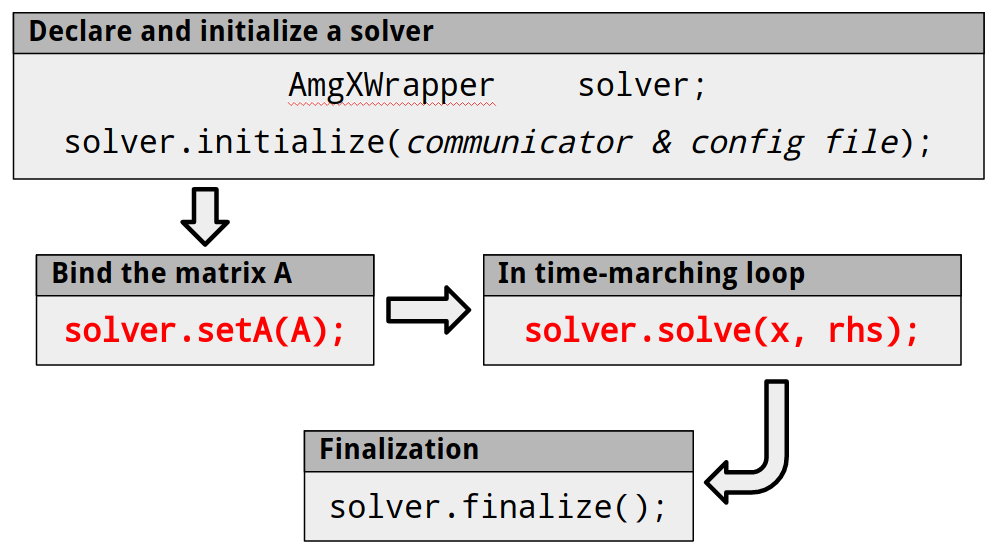
\includegraphics[width=0.6\linewidth]{amgxwrapper.png}
    \caption{Usage of AmgXWrapper in legacy PETSc applications}
    \label{fig:amgxwrapper}
\end{figure}

In addition to serve as a translation layer, AmgXWrapper also resolves an issue happens when CPUs and GPUs are both used in calculation.
It is common that HPC clusters have much more CPU cores than GPUs.
So CFD practitioners usually favor using all CPU cores and GPUs for computing.
However, most multi-GPU libraries were not developed for this use case.
Including AmgX, they expect users to use the same number for both MPI processes and GPUs.
AmgXWrapper provides matrix consolidation mechanism for use case when CPU cores and MPI processes are greater than available GPUs.
For example, most GPUs even nowadays do not have enough memory to host a whole 3D CFD problem.
So users may choose to use CPUs for solving forcing and velocity systems as they are not performance bottlenecks.
And they only use GPUs for pressure solvers to save GPU memory usage.
Therefore, it's natural for these users to use as many CPUs for forcing and velocity, so domain decomposition is done using the same number of MPI processes on CPUs.
When calling pressure solvers on GPUs, the number of subdomains do not match the number of GPUs, and this is when the matrix consolidation layer comes into play, as shown in figure \ref{fig:amgxwrapper-consolidation}.
Without the consolidation layer, several MPI processes would share one GPU, causing a resource competition.

\begin{figure}[H]
    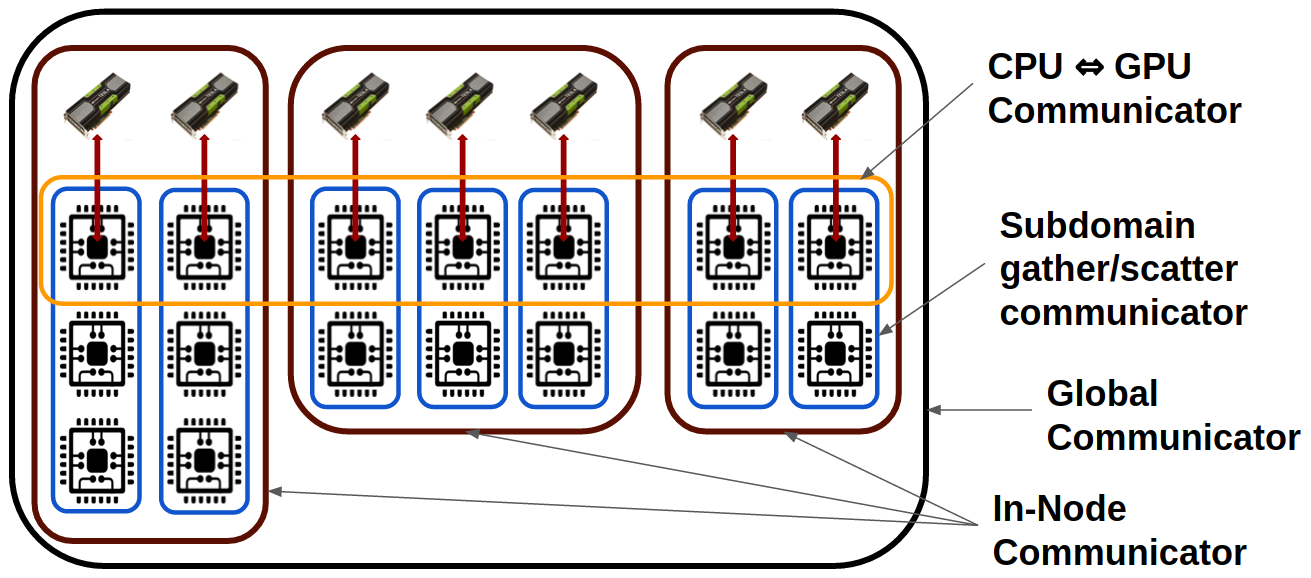
\includegraphics[width=0.6\linewidth]{amgxwrapper-consolidation.png}
    \caption{Graphic illustration of the consolidation layer in AmgXWrapper}
    \label{fig:amgxwrapper-consolidation}
\end{figure}

We will show the effect of the consolidation layer together with other performance benchmarks in section \ref{sec:petibm-perf}.
% vim:ft=tex

    \section{Verification and Validation}\label{sec:petibm-vv}
    %! TEX root = main.tex
This section shows cases for V\&V (verification and validation).
PetIBM is a baseline in PINN benchmarks, so its correctness must be confirmed.
These cases are: 2D and 3D Taylor\hyp{}Green vortex, 2D cylinder flows, 3D flow around a sphere, and 3D flow around an inclined flat plate.

\subsection*{Convergence test of 2D Taylor-Green vortex at $Re=100$}

The Taylor-Green vortex (TGV) represents a family of flows with a specific form of analytical initial flow conditions in 2D and 3D.
Specifically, 2D TGV problems with periodic boundary conditions have closed-form analytical solutions; hence, they usually serve as standard verification cases for CFD solvers. 
Here we used the following 2D Taylor-Green vortex to examine the order of convergence:
\begin{equation}\label{eq:tgv}
    \left\{
        \begin{aligned}
            u(x, y, t) &= V_0\cos(\frac{x}{L})\sin(\frac{y}{L})\exp(-2\frac{\nu}{L^2}t) \\
            v(x, y, t) &= - V_0 \sin(\frac{x}{L})\cos(\frac{y}{L})\exp(-2\frac{\nu}{L^2}t) \\
            p(x, y, t) &= -\frac{\rho}{4}V_0^2\left(cos(\frac{2x}{L}) + cos(\frac{2y}{L})\right)\exp(-4\frac{\nu}{L^2}t)
        \end{aligned}
    \right.
\end{equation}
$V_0$ represents the peak (and lowest) velocity at $t=0$;
$L$ is a scaling factor in the spatial domain;
$\nu$ and $\rho$ are kinematic viscosity and density, respectively.
$u$ and $v$ denote the velocity components in the $x$ and $y$ directions.
$p$ is the pressure.
The periodic boundary conditions are applied to $x=-L\pi$, $x=L\pi$, $y=-L\pi$, and $y=L\pi$.
As shown in the analytical solutions, the flow patterns do not change spatially, and only the amplitudes decay exponentially in time.

We used the following parameters for all our computational experiments: $V_0=L=\rho=1.0$ and $\nu=0.01$.
These parameters correspond to a Reynolds number of $Re=100$.

As the TGV problem only has periodic boundary conditions, there is no boundary discretization error in PetIBM that will taint the overall spatial convergence.
A 2nd-order grid convergence in space should therefore be expected.
The time marching schemes are Adams-Bashforth for the convection and Crank-Nicolson for the diffusion, so a 2nd-order convergence in time should also be observed.
Overall, the spatial-temporal convergence should be the 2nd-order.
Hence, we conducted a convergence test on spatial-temporal space for  convenience and simplicity.
The $L_2$ spatial-temporal error in this work is defined as:
\begin{equation}\label{eq:spt-err-def}
    \begin{aligned}
    L_{2,sp-t} \equiv &\sqrt{
        \frac{1}{L_x L_y T}
        \int\limits_{x} \int\limits_{y} \int\limits_{t} \lVert f - f_{ref} \rVert^2 \diff x \diff y \diff t
    } \\
    = &
    \sqrt{\frac{1}{N_x N_y N_t}\sum\limits_{i=1}^{N_x}\sum\limits_{j=1}^{N_y}\sum\limits_{k=1}^{N_t}\left(f^{(i, j, k)} - f_{ref}^{(i, j, l)}\right)^2}
    \end{aligned}
\end{equation}
$N_x$, $N_y$, and $N_t$ represent the number of cells on the $x$, $y$, and $t$ axis.
$f$ is the flow quantity of our interest, and $f_{ref}$ is the corresponding analytical solution.
The superscript $(i, j, k)$ denotes the value at the $(i, j, k)$ point in the discretized spatial-temporal space.
The characteristic cell size in a spatial-temporal sense is simply $\sqrt[3]{\frac{1}{N_x N_y N_t}}$, meaning the characteristic number of cells is $\sqrt[3]{N_x N_y N_t}$.

We ran simulations with $2^{n} \times 2^{n}$ cells for $i=4$, $5$, $\dots$, $10$.
The simulations ran from $t=0$ up to $t=100$, and we output the transient results every $2$ seconds of $t$.
The time step size $\Delta t$ did not follow a fixed refinement ratio.
Rather, it was refined based on the maximum allowed CFL number and whether it was a factor of $2$ (to output transient results).
The corresponding time step sizes were $\Delta t = 1.25\times 10^{-1}, 8\times 10^{-2}, 4\times 10^{-2}, 2\times 10^{-2}, 1\times 10^{-2}, 5\times 10^{-3}, 1.25\times 10^{-3}$.
The linear solvers for both velocity and pressure systems were solved with BiCGSTAB (biconjugate gradient stabilized method).
The velocity and pressure systems used a block Jacobi preconditioner and an algebraic multigrid preconditioner from AmgX.
At each time step, both solvers stopped when preconditioned residual reached $1\times 10^{-14}$.
The hardware contains 5 physical cores of Intel E5-2698 v4 and 1 V100 GPU.

Figure \ref{fig:petibm-tgv2d-re100-conv} shows the grid convergence results.
\begin{figure}[hbt!]
    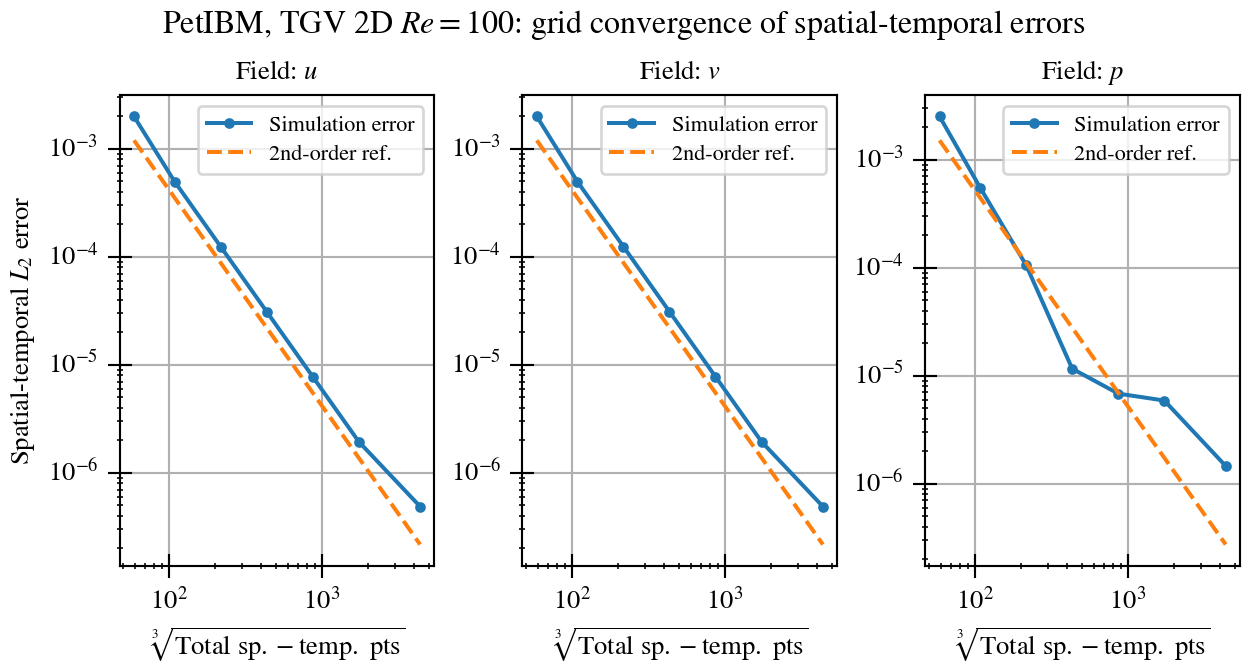
\includegraphics[width=0.75\linewidth]{tgv-2d-re100/petibm-tgv-2d-re100-convergence}
    \caption{PetIBM, 2D TGV, $Re=100$: spatial-temporal grid convergence}
    \label{fig:petibm-tgv2d-re100-conv}
\end{figure}
Both $u$ and $v$ velocities follow an expected 2nd-order convergence before machine roundoff errors become non-trivial at the $1024 \times 1024$ grid.
However, the pressure field does not follow such a nice convergence pattern.
After examining the log files, we determined that the cause was that AmgX did not solve the pressure systems to the tolerance we defined.
AmgX has a hard-coded stop mechanism when relative residuals (relative to the residual before the 1st iteration in a Krylov solver) reach the machine precision.
So while we configured the tolerance to be $1\times 10^{-14}$, the final preconditioned residuals of the pressure systems did not match this value.
On the other hand, the velocity systems were solved to the requested tolerance.

As we determined that the cause of the deviated convergence in pressure was irrelevant to the numerical method implementation, we concluded that the 2D TGV verification was successful.

\subsection*{Verification of 3D Taylor-Green vortex at $Re=1600$}

3D TGV problems have closed-form initial conditions but do not have closed-form analytical solutions.
These 3D TGV problems differ from 2D TGV cases due to the transition to turbulence.
Hence, it serves as a standard benchmark for turbulence simulations.
For example, see the campaign described in reference \cite{noauthor_1st_2012}. 
We compared the results to other published simulation data \cite{debonis_solutions_2013} in this verification.

The initial condition used was
\begin{equation}\label{eq:tgv3d-ic}
    \left\{
    \begin{aligned}
        u &=V_{0} \sin \left(\frac{x}{L}\right) \cos \left(\frac{y}{L}\right) \cos \left(\frac{z}{L}\right) \\
        v &=-V_{0} \cos \left(\frac{x}{L}\right) \sin \left(\frac{y}{L}\right) \cos \left(\frac{z}{L}\right) \\
        w &=0 \\
        p &=\frac{\rho V_{0}^{2}}{16}\left(\cos \left(\frac{2 x}{L}\right)+\cos \left(\frac{2 y}{L}\right)\right)\left(\cos \left(\frac{2 z}{L}\right)+2\right)
    \end{aligned}
    \right.
\end{equation}
We used $\rho = V_0 = L = 1$ and $\nu=0.000625$, corresponding to $Re \equiv \frac{V_0 L}{\nu} = 1600$.
The computational domain is $-L\pi$ to $L\pi$ for all three directions.

Due to the hardware required for high-resolution 3D DNS simulations for turbulent flow, we did not run the simulation with the spatial resolution suggested by reference \cite{noauthor_1st_2012}.
Our spatial resolution was $N_x=N_y=N_z=256$ with $\Delta t=0.01$.
The simulation ran up to $t=20$.
The hardware used was 128 physical CPU cores of AMD EPYC 7742 and 4 A100 GPUs (the 80GB variant).
It required about 250GB of memory, and the run time was 37 minutes.

Figure \ref{fig:petibm-tgv3d-re1600-val} shows that the mean kinetic energy qualitatively matches the reference data in \cite{noauthor_1st_2012} and \cite{debonis_solutions_2013}.
\begin{figure}[hbt!]
    \centering
    \begin{subfigure}[b]{0.45\textwidth}
        \centering
        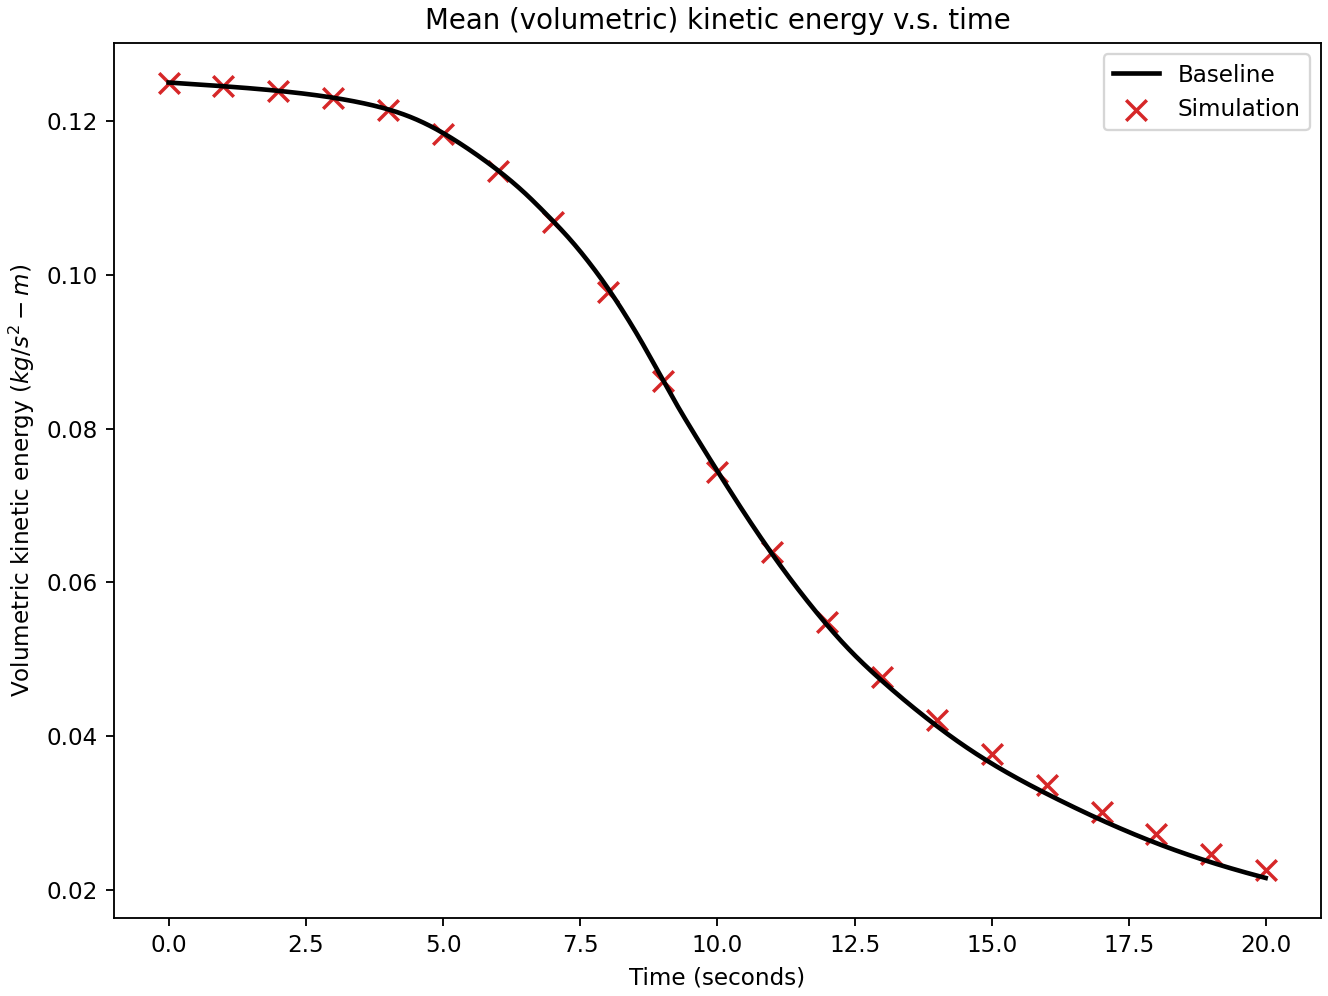
\includegraphics[width=\textwidth]{tgv-3d-re1600/mean-kinetic-energy}
        \caption{Mean kinetic energy}
        \label{fig:petibm-tgv3d-re1600-mean-energy}
    \end{subfigure}
    \hfill
    \begin{subfigure}[b]{0.45\textwidth}
        \centering
        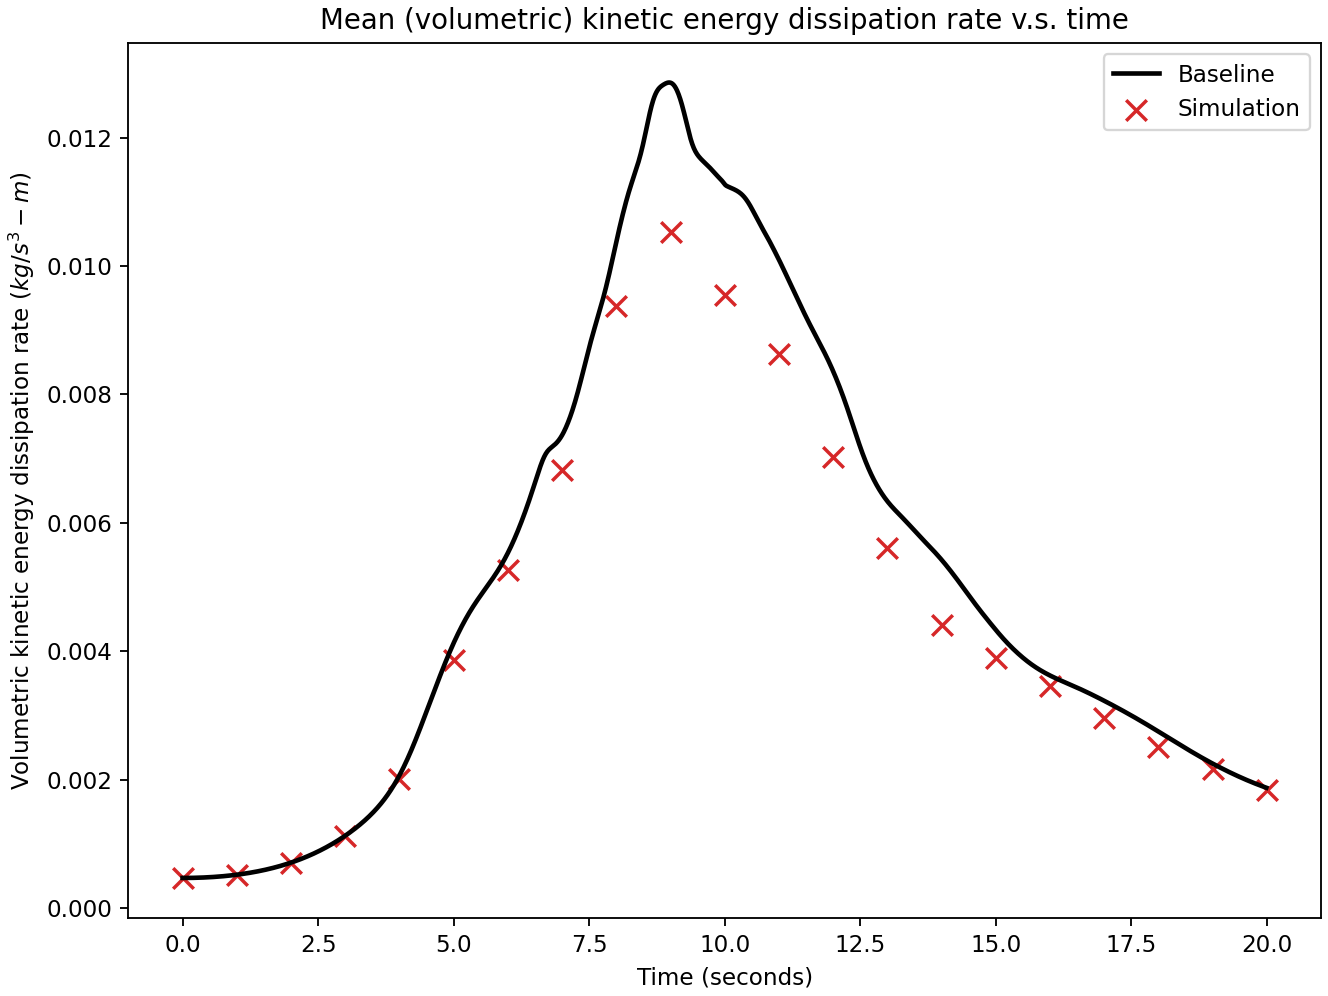
\includegraphics[width=\textwidth]{tgv-3d-re1600/mean-kinetic-energy-dissipation-rate}
        \caption{Mean kinetic energy dissipation rate}
        \label{fig:petibm-tgv3d-re1600-mean-energy-dissp}
    \end{subfigure}
    \caption{PetIBM, 3D TGV, $Re=1600$: validations}
    \label{fig:petibm-tgv3d-re1600-val}
\end{figure}
However, a visible mismatch exists in the mean kinetic energy dissipation rate.
Besides lower spatial resolution, another likely source of error is in the post-processing rather than in the numerical method implementation.
We calculated the dissipation rate using enstrophy, which requires post-processing steps due to using a staggered grid.
First, we applied the curl operator to the velocity defined on the staggered grid, and the resulting vorticity was also distributed staggered.
Next, we applied the linear interpolation operator and collected values from staggered grid points to cell centers.
Finally, we integrated the cell-centered vorticity using a simple 1st-order numerical integration.
Hence, we suspect that the post-processing largely contributed to the energy dissipation rate error.

Even some results from the campaign of references \cite{noauthor_1st_2012} and \cite{debonis_solutions_2013} show this level of mismatch in the dissipation rate.
Therefore, we conclude the 3D TGV verification at this point.
We do not claim that PetIBM's results match the reference data.
Nevertheless, it does not show any concerning problems in the comparison, either.

\subsection*{Validation and verification of 2D Cylinder flows}

In this work, a total of three different 2D cylinder flows were simulated: $Re=40$, $Re=100$, and $Re=200$.
In Williamson's stability categorization \cite{williamson_vortex_1996}, they correspond to the stable, 2D instability, and 2D to 3D transitioning regimes.
The cases of $Re=40$ and $Re=200$ were used for benchmarking PINNs.
Their results and V\&V can be found in chapter \ref{chap:pinn-cases}.
In this section, we only verify and validate our numerical solutions with $Re=100$.

The computational domain was $[-15$, $35]$ $\times$ $[-25$, $25]$ with a spatial discretization of $510$ $\times$ $298$.
Gridlines were stretched so that the cell size around the cylinder is about $\Delta x = \Delta y \approx 0.01\bar{6}$.
The time step size was $\Delta t = 0.01$.
The freestream condition of $u_{\infty}=1$ and $v_{\infty}=0$ were applied to the inlet, top, and bottom boundaries, while the outlet was convective BC.
The no-slip BC was applied to the cylinder surface.
The IC was $u_0=1$.
The configurations of the linear solvers in the velocity and the pressure systems were the same to those described in 2D TGV cases.
In addition, this case has an extra forcing system (equation \eqref{eq:dibpm-order2-2}), and it was solved using LU decomposition on CPUs through distributed SuperLU.
The hardware used was a node with 6 cores of intel i7-5930K and 1 K40 GPU.
It took about 10 minutes to finish the simulation.

\begin{table}[hbt!]
    \singlespacing
    \begin{threeparttable}[b]
        \begin{tabular}{lcc}
            \toprule
            & $C_{pb}$ \\
            \midrule
            PetIBM & -0.732   \\
            Williamson \& Roshko (1990) \tnote{1} & -0.736 \\
            \bottomrule
        \end{tabular}%
        \begin{tablenotes}
            \footnotesize
            \item [1] Through \cite{williamson_vortex_1996}. The third digit after the decimal point is an estimation as the value was obtained from digitizing a figure.
        \end{tablenotes}
        \caption[
            PetIBM, 2D Cylinder, $Re=100$: back suction coefficient validation with experimental data%
        ]{%
            2D Cylinder, $Re=100$: back suction coefficient validation with experimental data%
        }%
        \label{table:cylinder-2d-re100-cpb}
    \end{threeparttable}
\end{table}%
\begin{table}[hbt!]
    \singlespacing
    \begin{threeparttable}[b]
        \begin{tabular}{lcc}
            \toprule
            & $C_D$ & $St$ \\
            \midrule
            PetIBM & 1.36 & 0.174  \\
            Kim et al. (2001) \cite{kim_immersed-boundary_2001} & 1.33 & 0.165 \\
            Calhoun (2002) \cite{Calhoun2002} & 1.35\pm 0.014 & 0.175 \\
            Russell \& Wang (2003) \cite{Russell2003} & 1.38 \pm 0.007 & 0.169 \\
            Choi et al. (2007) \cite{choi_immersed_2007} & 1.34 \pm 0.011 & 0.164 \\
            \bottomrule
        \end{tabular}%
        \caption[%
            PetIBM, 2D Cylinder, $Re=100$: verification of drag coefficients and Strouhal number%
        ]{%
            Verification of net drag coefficients ($C_D$) and Strouhal numbers ($St$) for 2D cylinder flow at $Re=100$.%
        }%
        \label{table:cylinder-2d-re100-comparison-cd}
    \end{threeparttable}
\end{table}%

\begin{figure}[hbt!]
    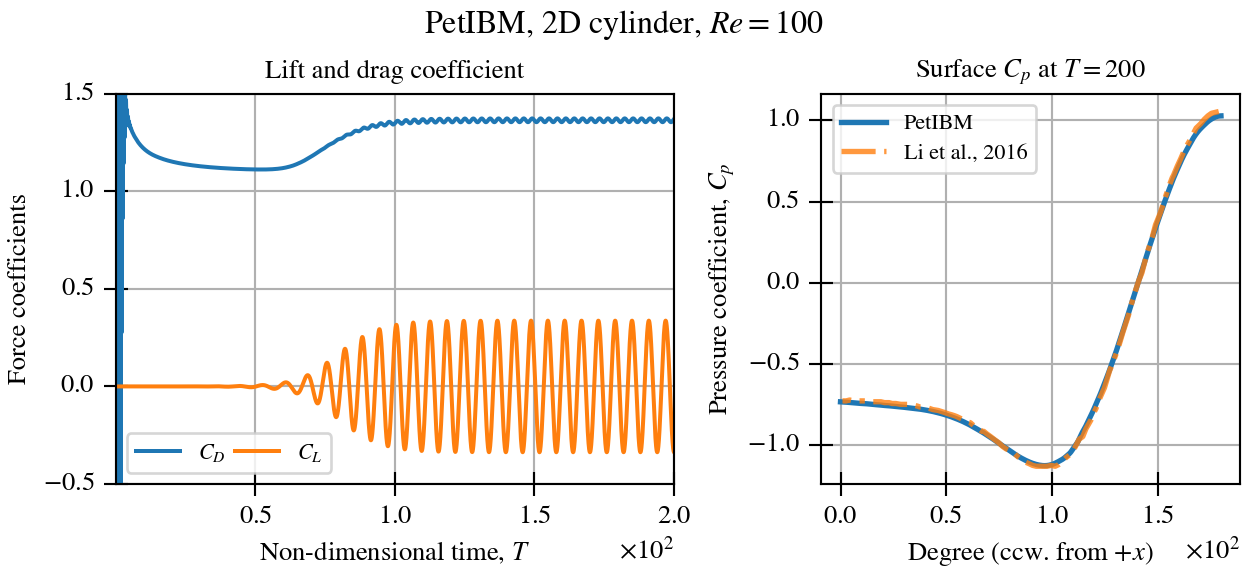
\includegraphics[width=0.95\linewidth]{cylinder-2d-re100/petibm-cylinder-2d-re100-val}
    \caption{PetIBM, 2D cylinder, $Re=100$: drag, lift, and pressure coefficients}
    \label{fig:petibm-cylinder-2d-re100-val}
\end{figure}

Table \ref{table:cylinder-2d-re100-cpb} shows the validation of the back suction coefficient, $C_{pb}$ (i.e., the surface pressure coefficient at the downstream end of the cylinder) against experimental data.
The drag coefficient and Strouhal number were verified with others' published numerical data and shown in table \ref{table:cylinder-2d-re100-comparison-cd}.
Figure \ref{fig:petibm-cylinder-2d-re100-val} shows the drag and lift coefficient with respect to time and the distribution of surface pressure coefficients.
The latter was verified against another published simulation result (see figure for the reference).

We determined that the V\&V for 2D cylinder flow at $Re=100$ was successful.

\subsection*{Validation of 3D flow around a sphere}

We validate the simulation results of 3D sphere flows at different Reynolds numbers.
These Reynolds numbers are $Re=50$, $100$, $150$, $200$, $250$, and $300$.
All cases used the same computational domain, $[-10$, $10]$ $\times$ $[-10$, $10]$ $\times$ $[-10$, $10]$, and the time step size $\Delta t=0.004$.
The corresponding grid sizes are $272$ $\times$ $82$ $\times$ $82$.
The BCs, ICs, and the linear solver configurations are the same as those in 2D cylinder flow at $Re=100$.

Figure \ref{fig:petibm-sphere3d-drag-val} shows the validation results against experimental data \cite{clift_bubbles_2013,roos_experimental_1971}.
\begin{figure}[hbt!]
    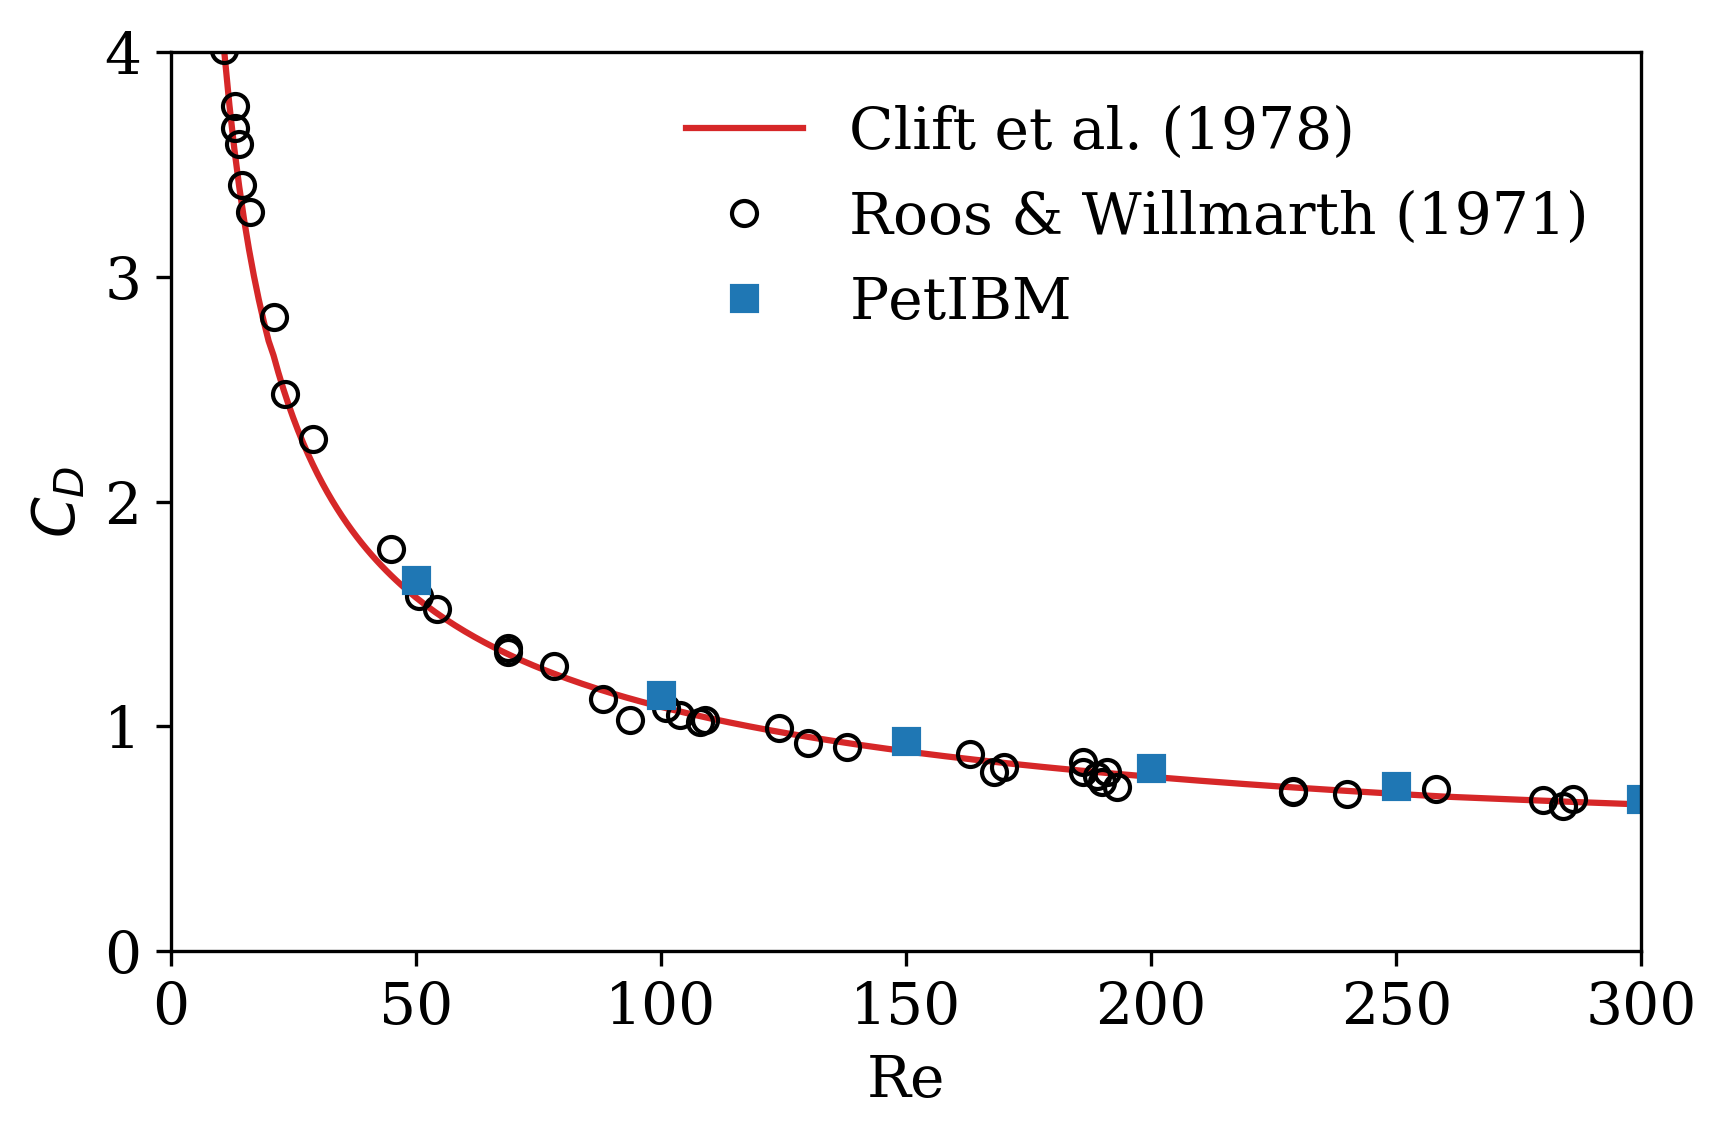
\includegraphics[width=0.6\linewidth]{sphere-3d/drag_coefficient}
    \caption[PetIBM, 3D sphere: drag coefficient validation]{
        PetIBM, 3D sphere: drag coefficient validation \cite{clift_bubbles_2013,roos_experimental_1971}
    }
    \label{fig:petibm-sphere3d-drag-val}
\end{figure}
We believe it is appropriate to call the validation of 3D sphere flow a success.

\subsection*{Validation of 3D flow around an inclined flat plate}

Lastly, we validate the solver using a 3D flow over an inclined flat plate at $Re=100$.
We tested with several AoA (angle of attack) and validated the results against the experimental data from reference \cite{taira_unsteadiness_2007}.
All cases had the same computational domain, $[-4$, $6.1]$ $\times$ $[-5$, $5]$ $\times$ $[-5$, $5]$, and the flat plate was located at $(0.1$, $1$, $1)$.
The spatial discretization is $192 \times 56 \times 86$, and the time step $\Delta t$ is $0.01$.
The BCs, ICs, and the linear solver configurations are the same as those in 2D cylinder flow at $Re=100$.

\begin{figure}[hbt!]
    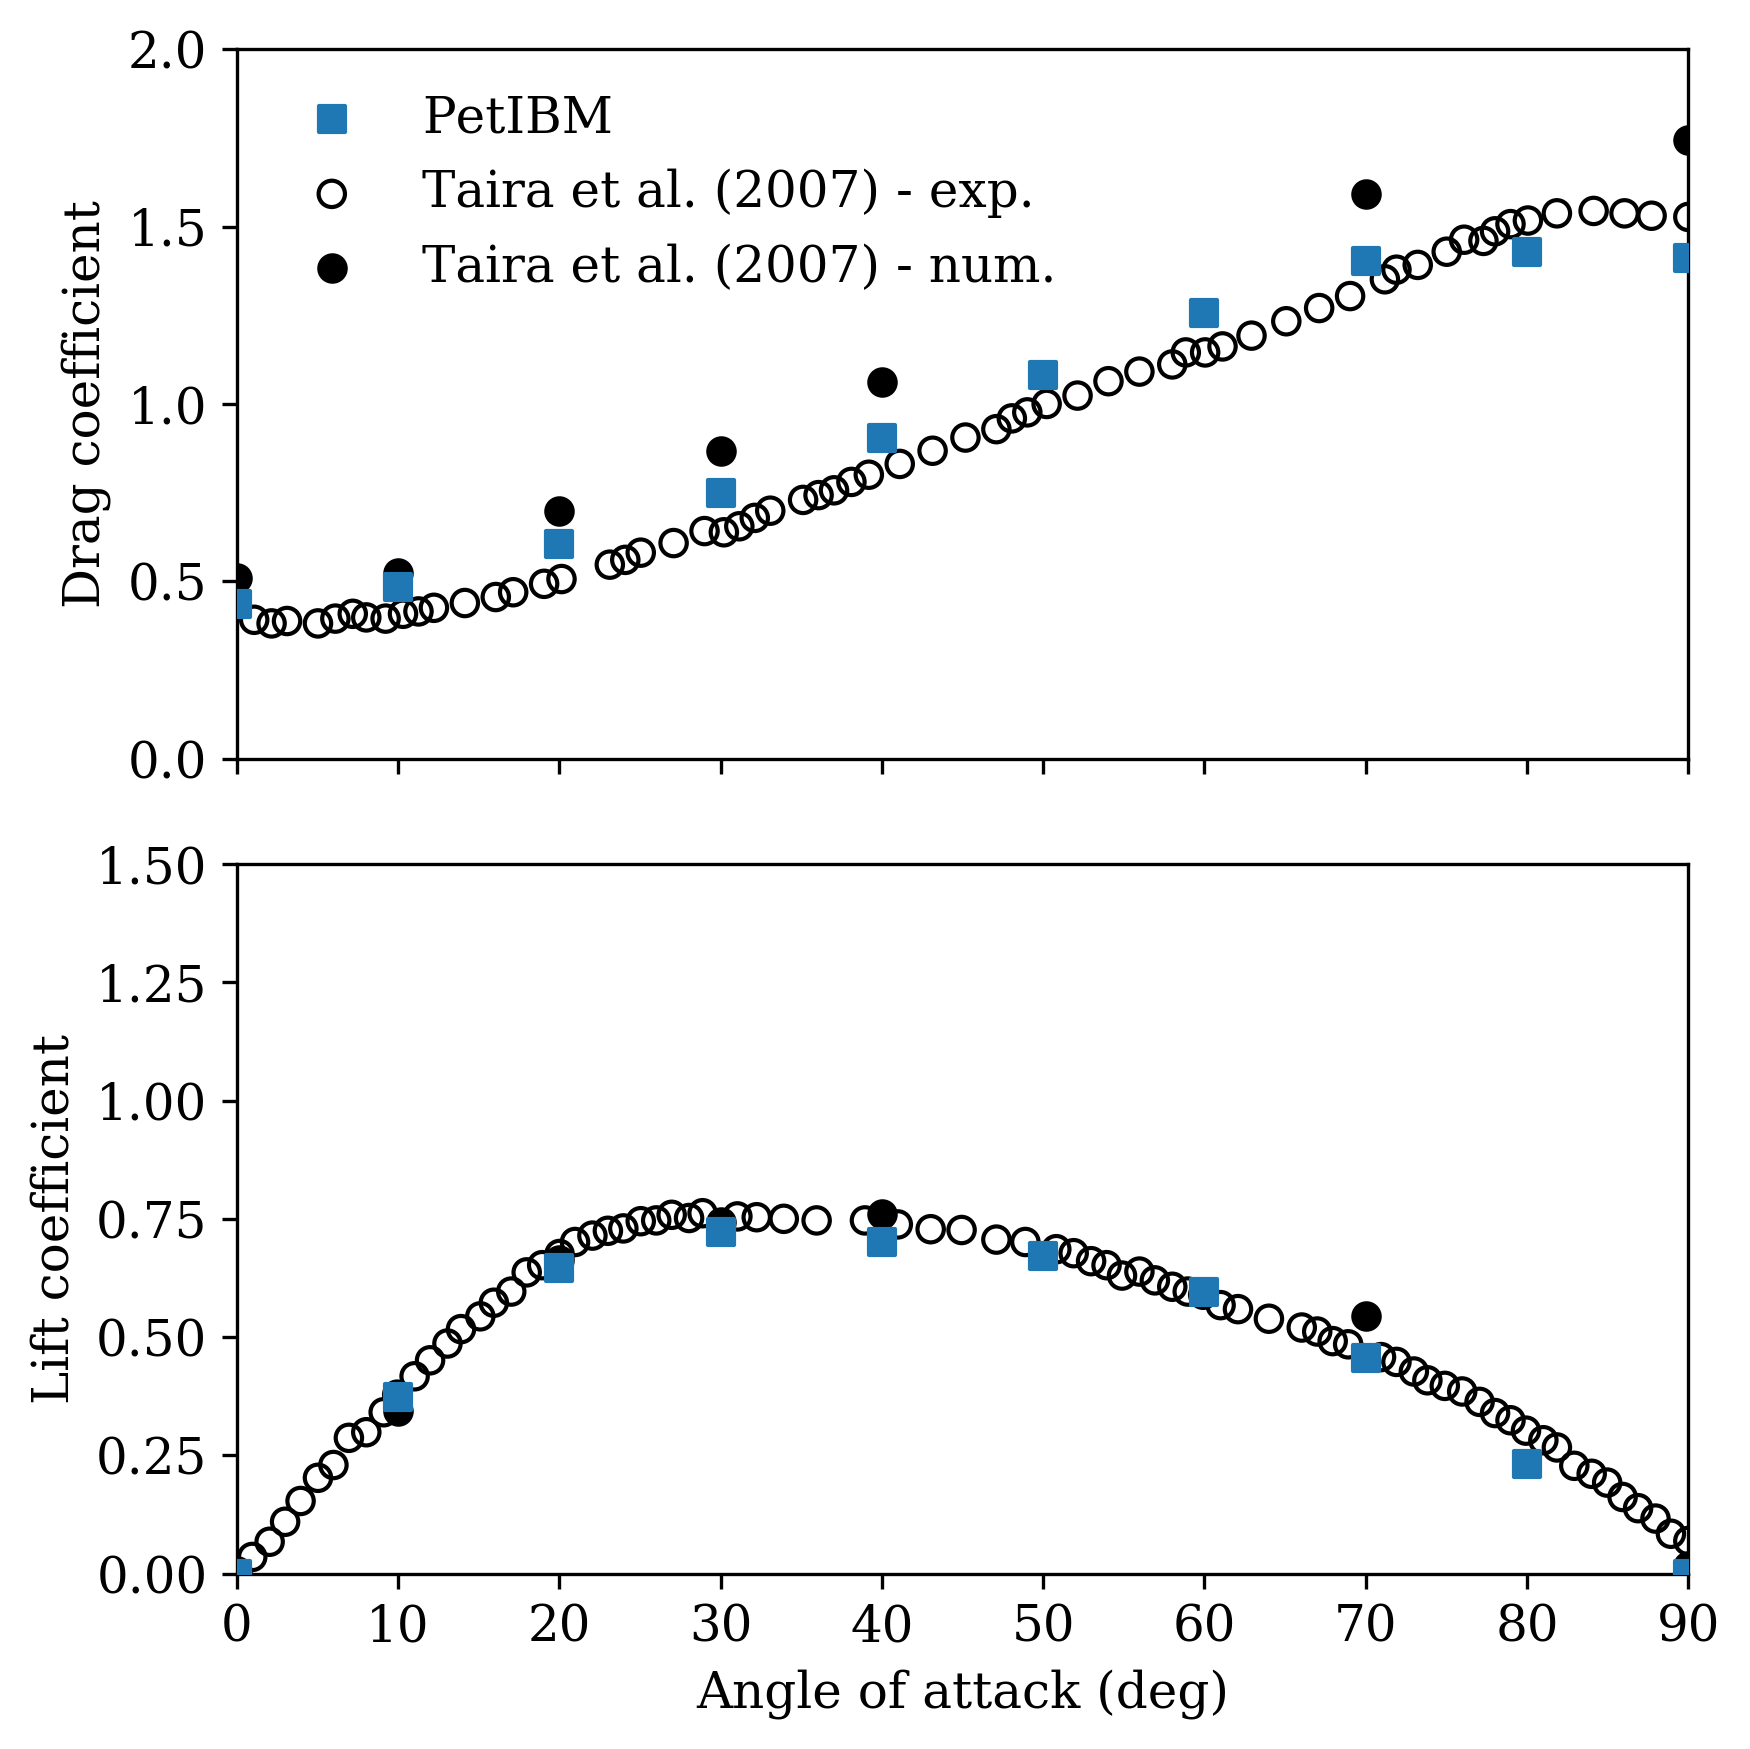
\includegraphics[width=0.6\linewidth]{plate-3d-re100/force_coefficients}
    \caption{PetIBM, 3D plate: drag and lift coefficient validation}
    \label{fig:petibm-plate3d-drag-lift-val}
\end{figure}
Figure \ref{fig:petibm-plate3d-drag-lift-val} shows that the experimental data matches our numerical simulation well.

% vim:ft=tex


    \section{Performance Benchmarks}\label{sec:petibm-perf}
    %! TEX root = main.tex

We first examined the performance of AmgXWrapper.
Figure \ref{fig:amgxwrapper-cons-1M} and \ref{fig:amgxwrapper-cons-15M} show the run time of solving Possion problems.
The former solves a smaller problem with $1$ million unknowns, and the latter has $15$ millions unknowns.
In each figure, on the left we have the performance before applying the consolidation mechanism in AmgXWrapper.
And on the right we show how the consolidation helps the performance.
The tests were done with NVIDIA V100 GPUs.

\begin{figure}[H]%
    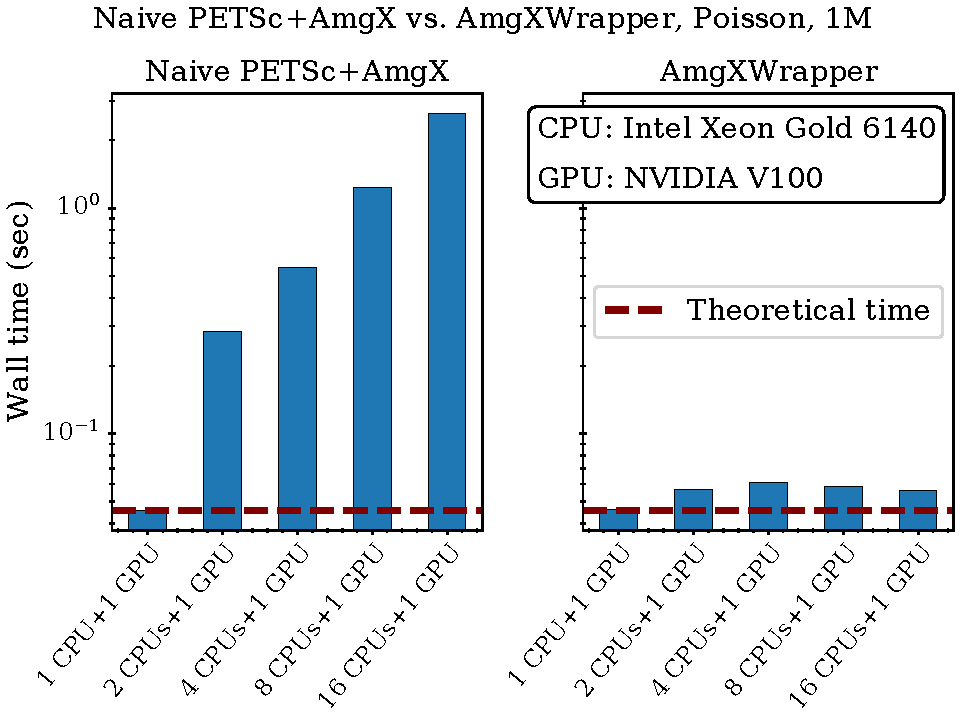
\includegraphics[width=0.6\linewidth]{amgxwrapper-consolidation-tests-poisson-1M}%
    \caption{AmgXWrapper benchmark: 3D Poisson problem w/ 1M unknowns and using 1 V100 GPU.}\label{fig:amgxwrapper-cons-1M}%
\end{figure}

\begin{figure}[H]%
    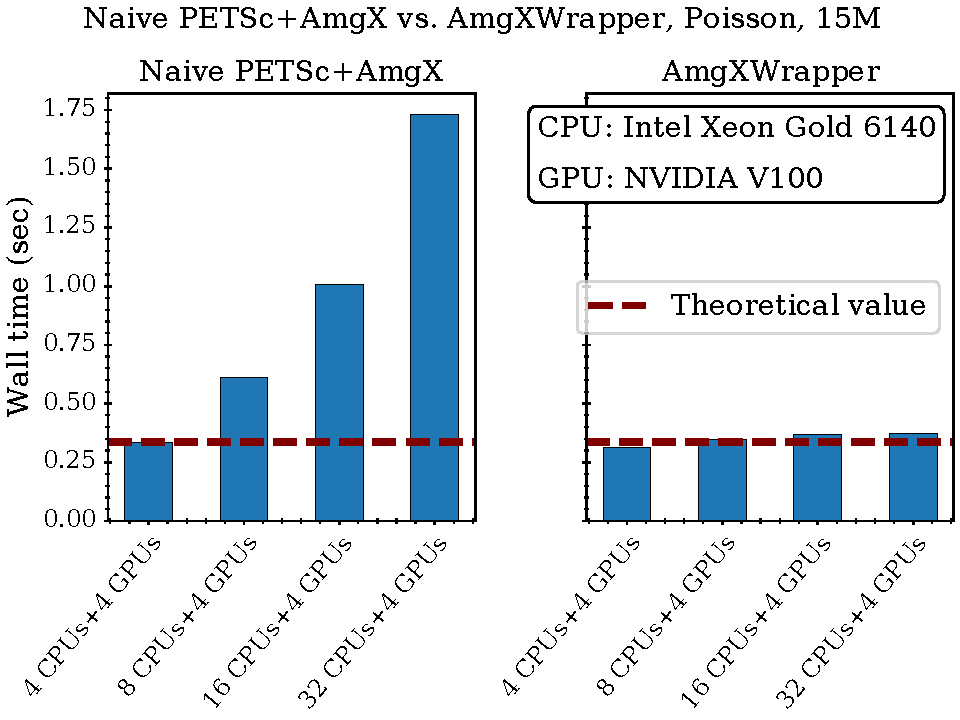
\includegraphics[width=0.6\linewidth]{amgxwrapper-consolidation-tests-poisson-15M}%
    \caption{AmgXWrapper benchmark: 3D Poisson problem w/ 15M unknowns and using 4 V100 GPUs.}\label{fig:amgxwrapper-cons-15M}%
\end{figure}

Bars in the figures represent the results of using different numbers of CPUs plus a fixed number of GPUs.
The smaller Poisson problem was solved with one GPU, while the larger problem was solved with 4 GPUs.
Using more CPUs speeds up the pre-processing stage, such as matrix creation because it means more subdomains and fewer unknowns per subdomain.
However, the run times of the solving stage should not be affected by the number of CPUs because the solver resides on GPUs completely, and we have a fixed number of GPUs.

Results in \ref{fig:amgxwrapper-cons-1M} and \ref{fig:amgxwrapper-cons-15M} show that this statement is not true for the plots on the left, that is, without consolidation. 
As more CPUs are used, run times grows linearly.
V100 was still the mainstream GPUs used on HPC clusters at the time of writing.
Yet the results show it was not designed for handling multiple tasks and does not handle well with resource competition.

The consolidation in the translation layer helps resolve the issue.
This mechanism consolidate and rearrange subdomains' matrices.
Rearranging is necessary as the performances of multigrid preconditioners may rely on the structures of submatrices on each GPU.
Plots on the right show that run times were close to a constant time regardless of how many CPUs were used.

The time used for consolidation was included in the solving stage shown in these two figures.
The smaller Poisson problem shows an overhead due to the consolidation.
However, for the larger problem, the overhead was not obvious as consolidation is a relative cheap operation compared to the actual solving. 

Next, in figure \ref{fig:amgxwrapper-speedups-15M} and \ref{fig:amgxwrapper-speedups-33M}, we show the speedups of GPU solvers versus CPU solvers on Poisson problems.
The former has $15$ millions of unknowns, while the latter has $33$ millions.
The plots also contains a visualization of the strong scaling.
The CPU tests used the conjugate-gradient (CG) solver from PETSc with the BoomerAMG preconditioner from Hypre.
The GPU tests used the CG solver and the classical multigrid preconditioner from AmgX.
Theoretically, these two configurations are comparable because AmgX's classical multigrid preconditioner was a re-implementation on GPU of BoomerAMG. 

\begin{figure}[H]
    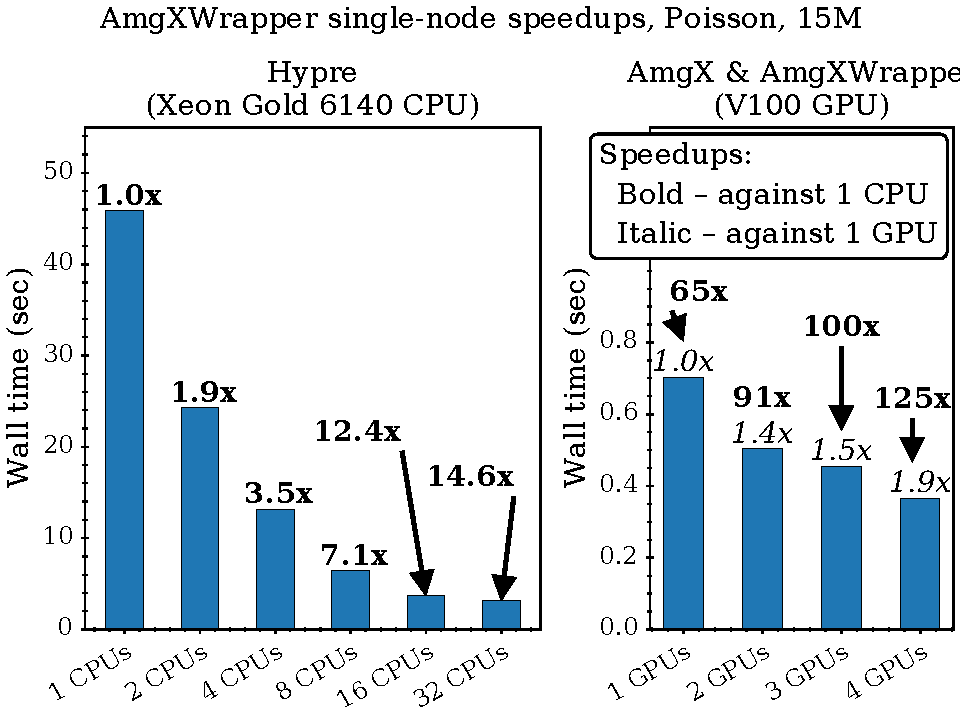
\includegraphics[width=0.6\linewidth]{amgxwrapper-proc-speedups-poisson-15M}
    \caption{Speedups of AmgXWrapper vs.\@ Hypre w/ 15M unknowns.}
    \label{fig:amgxwrapper-speedups-15M}
\end{figure}

\begin{figure}[H]
    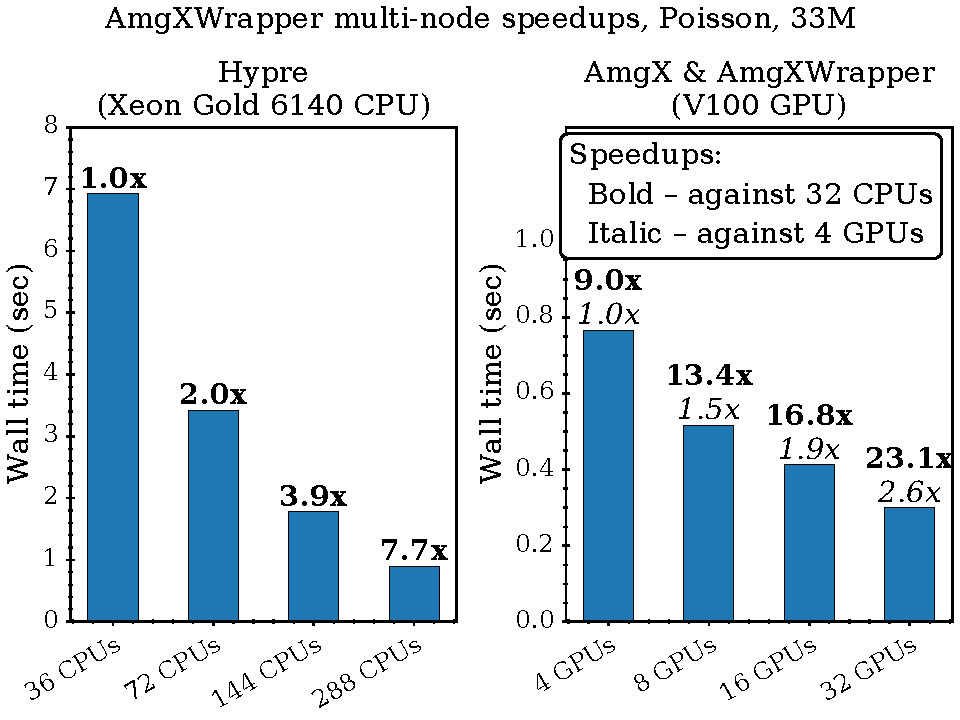
\includegraphics[width=0.6\linewidth]{amgxwrapper-node-speedups-poisson-33M}
    \caption{Speedups of AmgXWrapper vs.\@ Hypre w/ 33M unknowns.}
    \label{fig:amgxwrapper-speedups-33M}
\end{figure}

From the results, we observed a $65x$ speedup comparing 1 GPU to 1 CPU in the $15$-million problem and a $9x$ speedup comparing 4 GPUs to 36 CPUs in the $33$-million problem.
As a reference, at the time of writing, 4 V100 GPUs cost about $12$ thousand US dollars.
On the other hand, $36$ cores of CPUs consists of $2$ Xeon Gold 6140 chips, which cost around $2$ thousand US dollars\footnote{Xeon Gold 6140 was descontinued at the time or writing. The price we show here was the market value at the time, while the official suggested price for $2$ brand-new chips was around $4,800$ US dollars.}.
If we naively compare the results base on the monetary cost of the GPUs and CPUs, we would observe a speedup of about $1.5x$ (4 V100 GPUs versus 218 CPU cores).
However, as CPUs and GPUs work under different hardware configurations and setups, this monetary-based comparison is not fair in the real world.
For example, $6$ CPU chips may require $3$ complete computing nodes and an HPC cluster, while 4 V100 GPU can completely reside in one single workstation or even a personal desktop.
Under this argument, both the hardware cost and human labor cost (for maintenance) of CPUs will be much higher, and the speedups and cost saving from GPUs will be much more attractive.
Unfortunately, we were not able to get the cost estimation of a $3$-node HPC cluster and hence were not able to continue on the monetary cost comparisons.
Nevertheless, we hope our arguments can provide an impression on the hardware costs as these costs are often ignored in literature of performance benchmarks.

In terms of strong scaling, CPU solvers tended to show a better strong scaling.
For example, if we translate the speedup in the CPU results to strong scaling efficiencies for the smaller problem were about 95\%, 88\%, 88\%, 78\%, and 46\%, respectively.
And those of the larger problem were 100\%, 98\%, and 96\%.
In the GPU results, the strong scaling efficiencies of the small problem were 70\%, 50\%, and 48\%, while those of the larger problem were 75\%, 47\%, and 32\%.
From this viewpoint, CPU solvers give a better predictability on required resources and time-to-solutions. 

Finally, we were interested the actual performance gain in real flow simulation.
Figure \ref{fig:petibm-speedups-15M-small} and \ref{fig:petibm-speedups-15M-large} show the high-level performance profiling of PetIBM using a 3D flying-snake simulation \cite{krishnan_lift_2014,krishnan_cuibm_2017}.
The number of cells is $15$ millions, meaning there were about $45$ millions unknown in the velocity system and $15$ million unknowns in the pressure system.
The snake was discretized to $2,925$ Lagrangian points, meaning the forcing system has $8,775$ unknowns.

\begin{figure}[H]
    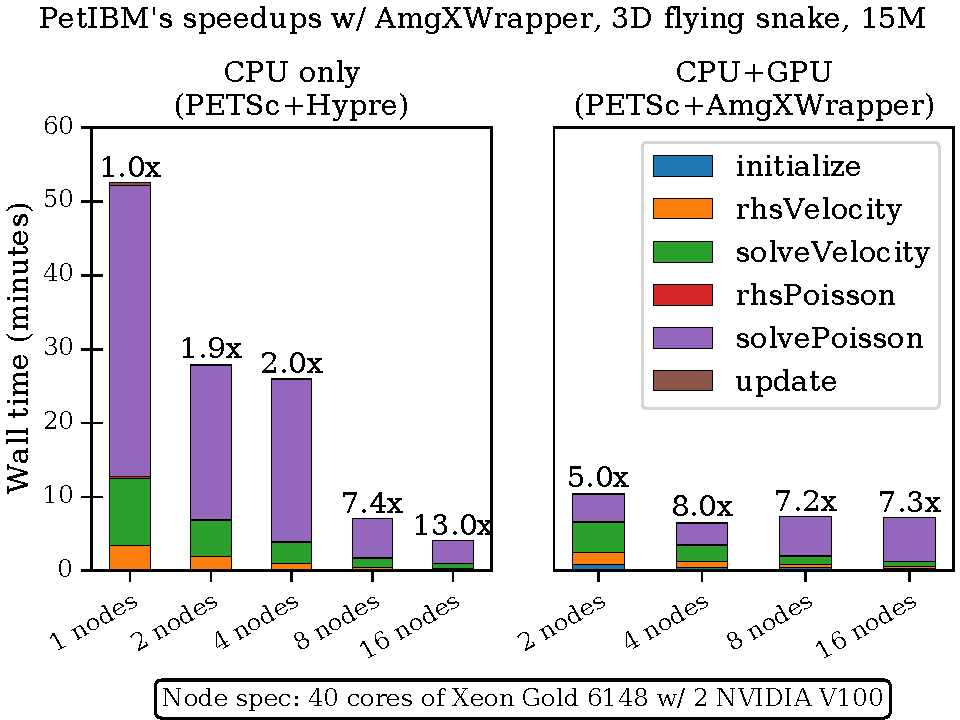
\includegraphics[width=0.6\linewidth]{petibm-speedups-scaling-small-gpu}
    \caption{Speedups of PetIBM: 2 V100 per node}
    \label{fig:petibm-speedups-15M-small}
\end{figure}

\begin{figure}[H]
    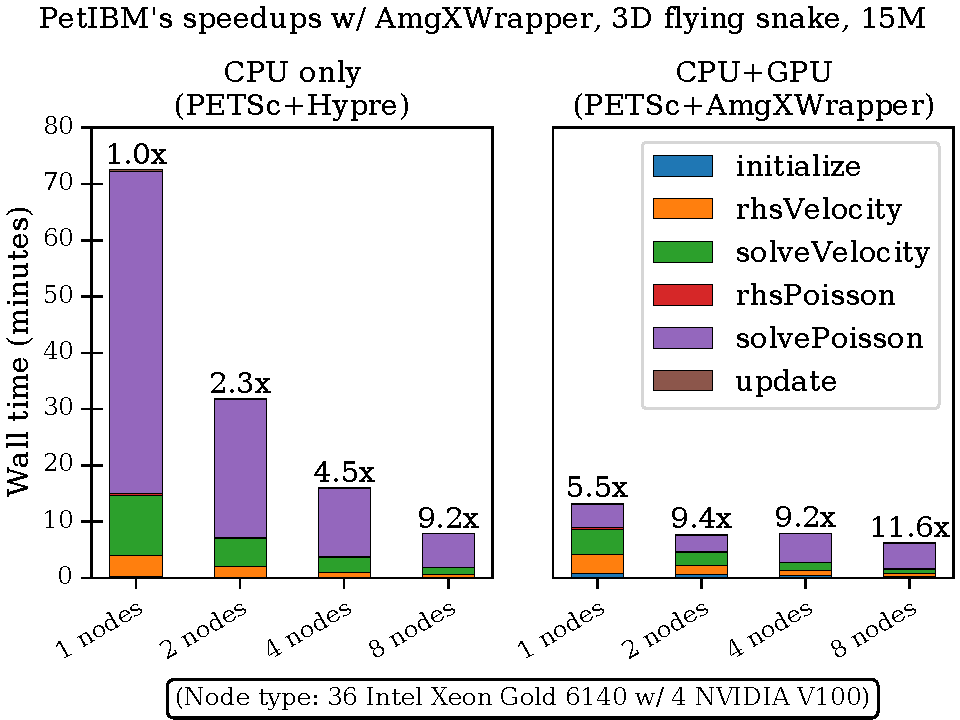
\includegraphics[width=0.6\linewidth]{petibm-speedups-scaling-large-gpu}
    \caption{Speedups of PetIBM: 4 V100 per node}
    \label{fig:petibm-speedups-15M-large}
\end{figure}

In CPU-only simulations, PetIBM solved velocity systems with the GAMG preconditioner and pressure systems with BoomerAMG preconditioner.
In CPU-GPU mixed simulations, the preconditioners for velocity and pressure systems are block-Jacobi and classical multigrid from AmgX, respectively.
The underlying Krylov solvers are the bi-conjugate gradient stabilized solver from either PETSc or AmgX.
The forcing systems in both types of simulations were solving by LU decomposition using distributed SuperLU.
This is the only part solved on CPU for the CPU-GPU mixed simulations.

The two figures show the performance speedups comparing pure-CPU and CPU-GPU-mixed simulations on two different clusters: one with 2 V100 per node, while the other one with 4 V100 per node.
We conducted the simulations on two different to ensure the results has generalizability.
The results from both clusters agree with each other.
We observed that one 4-GPU node or two 2-GPU nodes are equivalent roughly to 5 pure-CPU nodes.
The difference between the two clusters lies in that the 4-GPU nodes had less internode communication and hence had better performance and scalability.
% vim:ft=tex

\chapter{Physics-Informed Neural Networks}\label{chap:pinn}

    \section{Solving Workflow Overview}\label{sec:pinn-workflow-overview}

        \subsection{Overview}\label{sec:pinn-overview}
        %! TEX root = main.tex
Consider the incompressible Navier-Stokes equations in a spatial domain of $\vec{x}\in\Omega$ and a time range of $t\in[0$, $T]$:
\begin{subequations}\label{eq:orig-ns}
    \begin{empheq}[left=\left\{\,, right=\right.]{align}
        &\pdiff{\vec{u}}{t} + \left(\vec{u} \cdot \nabla\right) \vec{u}
            =
            -\frac{1}{\rho}\nabla p + \frac{1}{Re} \nabla^2 \vec{u}
            \label{eq:orig-ns-momentum} \\
        &\nabla \cdot \vec{u} = 0 \label{eq:orig-ns-cont}
    \end{empheq}
\end{subequations}
A solution to the Navier-Stokes equations is subject to IC and BCs:
\begin{equation}\label{eq:orig-ns-ic}
    \left\{
        \begin{array}{l}
            \vec{u}(\vec{x}, t=0) = \vec{u}_0(\vec{x}) \\
            p(\vec{x}, t=0) = p_0(\vec{x}) \\
        \end{array}
    \right.
    \text{,\ \ for }
    \vec{x} \in \Omega
\end{equation}
and
\begin{equation}\label{eq:orig-ns-bc}
    \left\{
        \begin{aligned}
            &\vec{u}(\vec{x}, t) = \vec{u}_{bc}(\vec{x}, t) \\
            &p(\vec{x}, t) = p_{bc}(\vec{x}, t)
        \end{aligned}
        \text{,\ \ for }
        \vec{x} \in \Gamma_{bc}
        \text{ and }
        t \in [0, T]
    \right.
\end{equation}
We only list the Dirichlet BCs to save space and for simplicity, as the treatment of Neumann BCs does not differ from treating PDEs in PINNs.

In the method of PINNs, the first step is to approximate the solutions of \eqref{eq:orig-ns} with a neural network model.
Let the network model name be $G$, of which the inputs are spatial coordinates $\vec{x}\equiv\begin{bsmallmatrix}x & y & z\end{bsmallmatrix}^\mathsf{T}$, time $t$, and a set of free parameters $\Theta$ that we need to determine later:
\begin{equation}\label{eq:G-network}
    \begin{bmatrix}
        \vec{u}(\vec{x}, t) \\ p(\vec{x}, t)
    \end{bmatrix}
    \approx
    G(\vec{x}, t; \Theta)
    =
    \begin{bmatrix}
        G^{\vec{u}} \\
        G^p
    \end{bmatrix}
    =
    \begin{bmatrix}
        G^u \\
        G^v \\
        G^w \\
        G^p
    \end{bmatrix}
\end{equation}
where $\vec{u}\equiv\begin{bsmallmatrix}u & v & w\end{bsmallmatrix}^\mathsf{T}$ is the velocity vector, and $p$ is the pressure.
In \eqref{eq:G-network}, we use a single network to predict both pressure and velocity fields.
Though it is possible to use separate networks for different fields, we keep \eqref{eq:G-network} this way for simplicity.
Also, later in this work, we will use $G^{\vec{u}}$, $G^u$, $G^v$, $G^w$, and $G^p$ to denote the predicted velocity vector, components, and pressure from $G$.
In this section, we will focus on the solution workflow \cite{dissanayake_neural-network-based_1994,lagaris_artificial_1998,cai_physics-informed_2021} and leave the mathematical expression of neural network models to section \ref{sec:mlp}.

The next step is to approximate the derivatives required for the differential equations.
For example, the continuity equation $\nabla \cdot \vec{u} = \pdiff{u}{x} + \pdiff{v}{y} + \pdiff{w}{z}$ requires the approximations for the 1st-order derivatives of velocity.
A possible approach is to rely on numerical differentiation.
For example, using finite difference, $\pdiff{u}{x}$ can be
\begin{equation*}
    \pdiff{u}{x} \approx \frac{G^u(x+\Delta x, \cdots)-G^u(x-\Delta x, \cdots)}{2\Delta x} 
\end{equation*}
Model $G$ is continuous and not defined on discretized space, so $x$ can be arbitrary coordinates in the domain.
And $\Delta x$ is a user-provided scalar as there is no grid.
However, we will not proceed with numerical differentiation. 
Being a continuous model and having a well-defined mathematical expression, $G$ gives us two more reasonable options.

The first option is to obtain analytical derivatives through symbolic differentiation or manual derivation.
For example, a very simple MLP network for a steady 2D flow may look like
\begin{equation}\label{eq:explicit-toy-mlp}
    \begin{aligned}
    &\begin{bmatrix}
        u &
        v &
        p
    \end{bmatrix}^\mathsf{T}
    \approx
    \begin{bmatrix}
        G^u &
        G^v &
        G^p
    \end{bmatrix}^\mathsf{T}
    =
    G(x, y; \Theta) \\
    = 
    &\begin{bmatrix}
    c_{11} \cos{\left(a_{11}x + a_{12}y + b_1\right)} + 
      c_{12} \cos{\left(a_{21}x + a_{22}y + b_2\right)} \\
    c_{21} \cos{\left(a_{11}x + a_{12}y + b_1\right)} + 
      c_{22} \cos{\left(a_{21}x + a_{22}y + b_2\right)} \\
    c_{31} \cos{\left(a_{11}x + a_{12}y + b_1\right)} + 
      c_{32} \cos{\left(a_{21}x + a_{22}y + b_2\right)} \\
    \end{bmatrix}
    \end{aligned}
\end{equation}
where $a_{ij}$, $b_i$, and $c_{ki}$ for $i$, $j=1$, $2$ and $k=1$, $2$, $3$ are free parameters in the model and belong to $\Theta$.
This MLP network is said to have one hidden layer with 2 neurons per layer and uses cosine for the activation function.
(Note that it is uncommon to use cosine for activation in real applications.)
We will formally introduce the definitions of these terms and the MLP's matrix form in section \ref{sec:mlp}.
Given the expression of \eqref{eq:explicit-toy-mlp}, we are able to obtain the derivatives.
Such as
\begin{equation}
    \begin{aligned}
    \pdiff{u}{x}
    \approx
    \pdiff{G^u}{x}
    =
    a_{11}c_{11}\cos\left(a_{11}x + a_{12}y + b_1\right) + a_{21}c_{12}\cos\left(a_{21}x + a_{22}y + b_2\right)
    \end{aligned}
\end{equation}
And the same concept applies to all higher-order derivatives.

Analytical derivatives were used in earlier literature when the networks might be just slightly more complicated than the one shown in \eqref{eq:explicit-toy-mlp}.
When the neural network models become more and more complicated, analytical derivatives become much less feasible, if not impossible.
Even modern hardware and symbolic differentiation software may not be able to obtain the analytical derivatives when $G$ has tens of thousands of free parameters and when the activation is not as simple as a cosine function.

Modern deep learning instead relies on the second option: automatic differentiation \cite{griewank_automatic_1988}.
Automatic differentiation is based on the chain rule and gives exact derivatives (exact with respect to actual computer intrinsic operations).
Section \ref{sec:ad} will talk about the fundamental concept of automatic differentiation.
At this point, we can just treat the automatic differentiation as a black box function that returns exact derivatives.
It requires fewer computing resources than symbolic differentiation and provides more accurate derivatives than numerical differentiation.

Moving on to the next step, once we obtain the desired derivatives, we substitute these derivatives into the governing PDEs, IC, and BCs.
For example, by substituting $G$ and corresponding derivatives to \eqref{eq:orig-ns}, \eqref{eq:orig-ns-ic}, and \eqref{eq:orig-ns-bc}, we get several residual functions
\begin{equation}\label{eq:residuals}
    \begin{array}{ll}
        \left\{
            \begin{array}{l}
            \hat{\vec{r}}_{m}(\vec{x}, t; \Theta) \equiv \frac{\partial G^{\vec{u}}}{\partial t}+(G^{\vec{u}} \cdot \nabla) G^{\vec{u}}+\frac{1}{\rho} \nabla G^p -\nu \nabla^{2} G^{\vec{u}} \\
            \hat{r_{c}}(\vec{x}, t; \Theta) \equiv \nabla \cdot G^{\vec{u}} 
            \end{array}
        \right. &
        \forall
        \left\{
            \begin{array}{l}
                \vec{x} \in \Omega \\ t \in [0, T]
            \end{array}
        \right. \\
        \left\{
            \begin{array}{l}
            \hat{\vec{r}}_{ic,\vec{u}}(\vec{x}; \Theta) \equiv G^{\vec{u}}(\vec{x}, t=0)-\vec{u}_0(\vec{x}) \\
            \hat{r}_{ic,p}(\vec{x}; \Theta) \equiv G^{p}(\vec{x}, t=0)-p_0(\vec{x})
            \end{array}
        \right. &
        \forall
        \vec{x} \in \Omega \\
        \left\{
            \begin{array}{l}
            \hat{\vec{r}}_{bc,\vec{u}}(\vec{x}, t; \Theta) \equiv G^{\vec{u}}-\vec{u}_{bc} \\
            \hat{r}_{bc,p}(\vec{x}, t; \Theta) \equiv G^{p}-p_{bc}
            \end{array}
        \right. &
        \forall
        \left\{
            \begin{array}{l}
                \vec{x} \in \Gamma_{bc} \\ t \in [0, T]
            \end{array}
        \right.
    \end{array}
\end{equation}
To make the expression cleaner, we omitted $\vec{x}$, $t$, and $\Theta$ in $G$.
Residual vectors $\hat{\vec{r}}_i$ and residual scalar $\hat{r}_i$, where $i$ denotes different residual sources, are functions of $\vec{x}$, $t$, and $\Theta$.
They are zero anywhere in the domain of interest only when the approximation solution $G$ perfectly fits in \eqref{eq:orig-ns}, \eqref{eq:orig-ns-ic}, and \eqref{eq:orig-ns-bc}.

The final step is to find a set of parameters $\vec{\theta}=\begin{bsmallmatrix}\theta_1 & \theta_2 & \cdots\end{bsmallmatrix}^\mathsf{T}$ that makes all residuals zero, i.e., when $\Theta=\vec{\theta}$, $G$ perfectly fits into \eqref{eq:orig-ns}, \eqref{eq:orig-ns-ic}, and \eqref{eq:orig-ns-bc}.
$\vec{\theta}$ then represents the common zero roots of all the residual functions in \eqref{eq:residuals} for all $\vec{x} \in \Omega$, $\vec{x} \in \Gamma_{bc}$, and $t\in[0$, $T]$.

Assume there are a total of $N_\Theta$ free parameters.
If residual functions in (\ref{eq:residuals}) are not complicated, and if $N_\Theta$ is small enough, we may numerically find the zero roots by solving a system of $N_\Theta$ nonlinear equations.
Such a system of nonlinear equations may be generated by enforcing the zero-residual conditions only on a set of $N_\Theta$ spatial-temporal points, i.e., $N_\Theta$ pairs of $\vec{x}$ and $t$.
However, this approach rarely results in an easy-to-solve system, given that $G$ is usually complicated and $N_\Theta$ is large.
Even for the toy model like \eqref{eq:explicit-toy-mlp}, the first-order derivatives are non-trivial.
If we further consider higher-order derivatives and the native nonlinearity in the PDEs, even this toy model results in a complicated nonlinear system. 
We do not even know if zero roots exist for this nonlinear system.

We instead relax the condition in PINNs.
We do not seek the zero roots of \eqref{eq:residuals} but just hope the desired set of parameters, $\theta$, makes the residuals sufficiently close to zero.
Also, note that the residual functions in \eqref{eq:residuals} are continuous in the domain and time range of our interest.
To make the optimization easier, we also limit ourselves to finding the minimal residuals at some spatial-temporal coordinates only, rather than asking for minimal residuals everywhere in the continuous space-time domain. 
In other words, the resulting optimization problem tries to find $\vec{\theta}$ that gives the minimal residuals on some spatial-temporal points.

Assume we have picked $N_{PDE}$ spatial-temporal points from $\vec{x}\in\Omega$ and $t\in[0$, $T]$, $N_{IC}$ points in $\Omega$ but with a fixed time $t=0$, and $N_{BC}$ points from $\vec{x} \in \Gamma_{bc}$ and $t\in[0$, $T]$.
We define the residuals at these points as \\
\begin{equation}\label{eq:residual-norms}
    \begin{aligned}
        & r_{m}(\Theta) \equiv \sum\limits_{i=1}^{N_{PDE}} \lVert\frac{\partial G_i^{\vec{u}}}{\partial t}+(G_i^{\vec{u}} \cdot \nabla) G_i^{\vec{u}}+\frac{1}{\rho} \nabla G_i^p -\nu \nabla^{2} G_i^{\vec{u}} \rVert^2 \\
        & r_{c}(\Theta) \equiv \sum\limits_{i=1}^{N_{PDE}} ( \nabla \cdot G_i^{\vec{u}} )^2 \\
        & r_{ic,\vec{u}}(\Theta) \equiv \sum\limits_{i=1}^{N_{IC}} \lVert G^{\vec{u}}(\vec{x}_i, t=0)-\vec{u}_0(\vec{x}_i) \rVert^2 \\
        & r_{ic,p}(\Theta) \equiv \sum\limits_{i=1}^{N_{IC}} ( G^{p}(\vec{x}_i, t=0)-p_0(\vec{x}_i) )^2 \\
        & r_{bc,\vec{u}}(\Theta) \equiv \sum\limits_{i=1}^{N_{BC}} \lVert G_i^{\vec{u}}-\vec{u}_{bc} \rVert^2 \\
        & r_{bc,p}(\Theta) \equiv \sum\limits_{i=1}^{N_{BC}} ( G_i^{p}-p_{bc} )^2
   \end{aligned}
\end{equation}
where $\begin{bsmallmatrix}G_i^{\vec{u}} & G_i^p\end{bsmallmatrix}^\mathsf{T} = G(\vec{x}_i, t_i; \Theta)$, and $\lVert\cdot\rVert$ denotes $l_2$ norms.

One approach to interpret the optimization problem is
\begin{equation}\label{eq:hard-constraint-loss}
    \begin{aligned}
    &\vec{\theta} = \operatorname*{arg\,min}\limits_{\Theta} \left[r_m(\Theta) + r_c(\Theta)\right] \\
    \text{ subject to } &r_{ic,\vec{u}}=r_{ic,p}=r_{bc,\vec{u}}=r_{bc,p}=0
    \end{aligned}
\end{equation}
This is a constrained optimization problem.
Only residuals from PDEs are relaxed, and residuals from BCs and IC must be exactly zero.
Though exactly satisfied BCs and IC sound attractive, optimization with hard constraints is much more difficult than unconstrained optimization.
And optimization methods may not be general enough for arbitrary types of BCs and arbitrary computational domains.
This approach was used in, for example, references \cite{lagaris_artificial_1998,McFall2009,mcfall_solving_2010,berg_unified_2018} for limited types of PDEs and applications.

Alternatively, most recent reports of PINNs used soft constraints, that is
\begin{equation}\label{eq:total-residual}
    \vec{\theta} = \operatorname*{arg\,min}\limits_{\Theta} \left[
        r_m(\Theta) + r_c(\Theta) + r_{ic,\vec{u}}(\Theta) + r_{ic,p}(\Theta) + r_{bc,\vec{u}}(\Theta) + r_{bc,p}(\Theta)
    \right]
\end{equation}
Though the optimized $\vec{\theta}$ does not guarantee that IC and BCs are satisfied, \eqref{eq:total-residual} is easier to solve and to be generalized to different PDEs, BCs, or applications.
In the terminology of optimization, \eqref{eq:total-residual} is called the loss function or objective.
Residuals from different sources are called loss terms.

In practice, a more general form of \eqref{eq:total-residual} is
\begin{equation}\label{eq:total-residual-weighted}
    \begin{aligned}
        \vec{\theta}
        &=
        \operatorname*{arg\,min}\limits_{\Theta} r(\Theta)  \\
        &=
        \operatorname*{arg\,min}\limits_{\Theta} \sum \alpha_i r_i(\Theta)
    \end{aligned}
\end{equation}
where $i$ denotes different loss terms in \eqref{eq:residual-norms}.
Each loss term is weighted before being aggregated to the final loss.
To our best knowledge, there is not yet a standard or guideline for how to properly configure $\alpha_i$.
It is common to see $\alpha_i=1$ in the literature.

If there exist zero roots that make all residuals in \eqref{eq:residual-norms} zero, then a perfect optimization method will find them from either \eqref{eq:hard-constraint-loss}, \eqref{eq:total-residual}, or \eqref{eq:total-residual-weighted}.
This hope is surely unrealistic.
First, zero roots' existence is not guaranteed.
Second, the hypersurface of the aggregated loss, $r(\Theta)$, in the vector space of $\Theta$ is usually neither convex nor concave, making it difficult to find the global minimum.
Even a simple 1D linear Burger's equation with an MLP of around \num{7850} free model parameters shows a complicated hypersurface of $r(\Theta)$ \cite{krishnapriyan_characterizing_2021}.
While finding zero roots or the global minimum on the hypersurface of $r(\Theta)$ is difficult, practitioners of PINNs just assume the local minimums of $r(\Theta)$ are good and small enough.

This poses a fundamental difference between conventional CFD schemes and PINNs: the former seeks exact zero roots to make residuals zero, while the latter just {\it hopes} to make residuals as small as possible.
It is thus reasonable to doubt PINNs' accuracy compared to conventional schemes.

Nevertheless, finding optimized $\vec{\theta}$ concludes the workflow of data-free PINNs for solving PDEs.
Figure \ref{fig:pinn-workflow} shows a graphical illustration of the workflow.
\begin{figure}[hbt!]
    \includegraphics[width=\linewidth]{figs/pinn.tikz} 
    \caption{A graphical demonstration of workflow in PINNs}
    \label{fig:pinn-workflow}
\end{figure}

The optimization process is done with the Adam optimizer \cite{kingma_adam_2017} in this work, together with a batched approach described in the next section.
% vim:ft=tex


        \subsection{Batched Training}\label{sec:batched-training}
        %! TEX root = main.tex

Compared to solving $N_\Theta$ nonlinear equations directly, an optimization problem of \eqref{eq:total-residual} or \eqref{eq:total-residual-weighted} allows us to use any number of spatial-temporal points.
That is, there is no limitation on the magnitude of $N_{PDE}$, $N_{BC}$, and $N_{IC}$.
This eases the need for computational resources.
In data-free PINNs, these spatial-temporal points are called training points or training data.
They are spatial-temporal coordinates where we evaluate the residuals of PDEs, IC, and BCs.
While training points may be generated manually and intentionally positioned at desired locations (just like meshing in conventional CFD simulations), it is more common to generate them by selecting coordinates randomly using a uniform density function. 

The ability to use arbitrary numbers of training points helps the generalizability of a trained PINNs model.
When more training points are involved in \eqref{eq:residual-norms} and hence \eqref{eq:total-residual-weighted}, the minimal residuals are achieved at more locations in the domain. 
Ultimately, with unlimited training points evenly distributed in the domain, optimizing the discretized residuals in \eqref{eq:residual-norms} becomes optimizing continuous residual functions in \eqref{eq:residuals}. 
And the resulting optimal parameters, $\vec{\theta}$, will make $G$ a more accurate approximation solution to the whole domain of $\Omega$ and $t\in[0$, $T]$.

More points also mean a higher computational cost.
Batched training is thus utilized to reduce the cost.
For example, if using an iterative optimization method (such as the gradient-descent or Adam optimizer), we can always generate a new batch of training points for a new iteration to evaluate the discretized residuals.
After a significant number of iterations, the total number of training points involved in optimization will also be significant.
Once the model is trained, theoretically, it is capable of giving accurate predictions at any location and time.

In practice, however, it is not a cheap task if thousands or even more random points have to be generated on the fly at each iteration.
We instead generated a fixed amount of training points before the optimization and only used a batch of them in each iteration.
For example, to use $N_{PDE}$ points to evaluate the PDE residuals at each iteration, we may generate $N_{PDE}\times 1000$ points in advance and divide them into $1000$ batches.
If we run an optimizer for 1 million iterations, each batch is repeated every 1000 iterations.

Theoretically, each batch should have similar statistical properties and give a similar gradient vector under fixed model parameters.
That is
\begin{equation}
\left.\nabla_\theta r(\Theta) \right|_{\vec{x}, t \in \mathcal{X}_1} \sim
\left.\nabla_\theta r(\Theta) \right|_{\vec{x}, t \in \mathcal{X}_2} \sim
\cdots
\end{equation}
where $\mathcal{X}_i$ for $i=1$, $2$, $\cdots$ represents the $i$-th batch of the training points.
These gradients are used to update $\vec{\theta}$ in iterative optimization methods.
In other words, the hypersurface of $r(\Theta)$ is expected not to change significantly from iteration to iteration when using different batches of points to evaluate it.
However, whether this statement is true may depend on the number of points in each batch: the number of points should be large enough to have similar statistical properties across different batches.

In PINNs, as the training points are randomly sampled from the computational space-time domain, the number of points in a batch should be large enough to cover all over the domain.
Otherwise, for example, if one batch mostly covers the inflow region of a cylinder flow while the next batch covers mostly the wake region behind the cylinder, then the hypersurface of the PDE residuals will change significantly.
This change of the hypersurface from iteration to iteration may slow down the convergence.
In the later benchmarks, we would like to examine the effect of batch sizes, i.e., the number of points in each batch. 

% vim:ft=tex


        \subsection{Adaptive Loss Aggregation}\label{sec:loss-annealing}
        %! TEX root = main.tex
In equation \eqref{eq:total-residual-weighted}, each individual loss term is weighted.
However, how to properly assign the weights is still and open question.
In references \cite{jin_nsfnets_2020,wang_understanding_2021}, the authors proposed an annealing approach to change these weights in an adaptive fashion during the optimization process.
However, these adaptive approaches have not been further tested by more works.
In this work, part of the benchmarks will cover the performance of the adaptive weight strategy proposed in \cite{jin_nsfnets_2020}.

Jin et al. \cite{jin_nsfnets_2020} proposed the following annealing loss aggregation algorithm for iterative optimization methods:
\begin{equation}
    r^k(\Theta) = r_{PDE}^k(\Theta) + 
        \left(\left(1-\lambda\right)\alpha^k + \lambda\alpha^{k+1}\right)r_{BC}^k(\Theta) + 
        \left(\left(1-\lambda\right)\beta^k + \lambda\beta^{k+1}\right)r_{IC}^k(\Theta)
\end{equation}
where $k$ denotes the $k$-th iteration in an iterative optimization method.
The subscript $PDE$, $BC$, and $IC$ denote the loss contributions from the residuals of PDEs, BCs, and IC.
$\lambda$ is a user-provided parameter to control the moving average of the current and the previous weights.
The concept of this adaptive approach is to make the gradients of each loss term comparable.
When using the gradient-descent method and its derived methods, the magnitude of each loss term is reduced with a similar rate.
And
\begin{equation}
    \alpha^{k+1} = \frac{\overline{\lvert\nabla_\Theta r_{PDE}^k(\Theta)\rvert}}{\overline{\lvert\nabla_\Theta r_{BC}^k(\Theta)\rvert}}
    \text{\ \ \ \ and\ \ \ \ }
    \beta^{k+1} = \frac{\overline{\lvert\nabla_\Theta r_{PDE}^k(\Theta)\rvert}}{\overline{\lvert\nabla_\Theta r_{IC}^k(\Theta)\rvert}}
\end{equation}
$\lvert\cdot\rvert$ denotes the element-wise absolute values of a vector.
$\overline{\lvert\cdot\rvert}$ is the mean values of these absolute values.

The following expression better represents the actual implementation in our code:
\begin{equation}
    \begin{aligned}
        &\zeta^k =
            \overline{\lvert\nabla_\Theta r_{m,u}^k(\Theta)\rvert} +
            \overline{\lvert\nabla_\Theta r_{m,v}^k(\Theta)\rvert} +
            \overline{\lvert\nabla_\Theta r_{m,w}^k(\Theta)\rvert} +
            \overline{\lvert\nabla_\Theta r_{c}^k(\Theta)\rvert} \\
        &\alpha^{k+1} = 
            \frac{\zeta^k}{\overline{\lvert\nabla_\Theta r_i^k(\Theta)\rvert}} \\
        &r^k(\Theta) = r_m^k(\Theta) + r_c^k(\Theta) + 
            \sum\limits_{i} \left(\left(1-\lambda\right)\alpha_i^k + \lambda\alpha_i^{k+1}\right) r_i^k(\Theta)
    \end{aligned}
\end{equation}
where $r_{m,u}^k$, $r_{m,v}^k$, and $r_{m,w}^k$ are the $u$-, $v$-, and $w$-component in the residual vector of the momentum equations at $k$-th iteration.
And subscript $i$ denotes different loss terms, excluding $r_m(\Theta)^k$ and $r_c(\Theta)^k$.
In this work, $\lambda$ is fixed at $0.1$ for all cases using annealing loss aggregation.
% vim:ft=tex

    \section{Deep Neural Network Modeling}\label{sec:pinn-dnnm}

        \subsection{Multilayer Perceptron Networks}\label{sec:mlp}
        %! TEX root = main.tex

In the previous section, $G$ denotes a neural network model (or any mathematical model) that predicts flow quantities at given spatial-temporal coordinates.
In this section, we would like to introduce the mathematical expression of the most common neural network model in data-free PINNs: MLP (multilayer perceptron) networks.

The universal approximation theorem \cite{hornik_approximation_1991} states that large-enough MLP networks can approximate any smooth function.
This theorem justifies the use of MLP networks as PDEs' approximate solutions.
These PDEs include the Navier-Stokes equations, which are the primary governing equations for CFD.\footnote[0]{Though the existence of the smooth solutions for the Navier-Stokes equations is not yet proved, as CFD practitioners, we usually ignore this theoretical fact.}

Figure \ref{fig:mlp-graph} is a commonly seen graphical illustration of how MLP works.
\begin{figure}[hbt!]
    \singlespacing
    \includegraphics[width=0.95\linewidth]{figs/mlp.tikz}
    \caption{Graphical illustration of MLP networks}
    \label{fig:mlp-graph}
\end{figure}
To avoid introducing more mathematical symbols, in this section and figure \ref{fig:mlp-graph}, we reuse the notation from the previous section.

An MLP network is fundamentally a series of linear-nonlinear mapping pairs:
\begin{equation}\label{eq:mlp-formula}
    \begin{array}{ll}
        \vec{h}^0 \equiv \begin{bmatrix} \vec{x} \\ t \end{bmatrix} & \\
        \vec{h}^k = \sigma_{k-1}\left(A^{k-1}\vec{h}^{k-1}+\vec{b}^{k-1}\right)\text{,} & 1 \le k \le N_l \\
        \vec{h}^{N_l+1}\equiv \begin{bmatrix} G^{\vec{u}} \\ G^p \end{bmatrix} = \sigma_{N_l}\left(A^{N_l}\vec{h}^{N_l}+\vec{b}^{N_l}\right) &
    \end{array}
\end{equation}
$\vec{h}^k$ is called a hidden layer or a latent space vector.
$\sigma_{k}$ is a chosen element-wise nonlinear function.
$A^{k}$ and $\vec{b}^k$ for $k=0$ to $k=N_l$ are parameter matrices and vectors that consist of free model parameters.
In other words, $\Theta=\left\{A^0, \vec{b}^0, A^1, \vec{b}^1, \cdots \right\}$.
$N_l$ denotes the number of hidden layers, and $N_n$ in figure \ref{fig:mlp-graph} represents the number of elements in each hidden layer, $\vec{h}^k$.
Elements in $\vec{h}^k$ are often called neurons in deep learning.
Theoretically, $N_n$ does not have to be constant.
Each $\vec{h}^k$ can have different $N_n$.
However, as there is no clear guideline on specifying variate $N_n$ for PINNs, most reports in PINNs just use a constant $N_n$ across hidden layers.
We follow the same approach in this work.

$A^k$ and $\vec{b}^k$ are the free parameters we want to determine in the optimization step (i.e., equation \eqref{eq:total-residual-weighted}).
$N_l$ and $N_n$ are also parameters that control the complexity and accuracy of an MLP network.
However, they are determined by users rather than by optimization.
These parameters are called hyperparameters---they are not counted in the degrees of freedom of a mathematical model.

The element-wise nonlinear functions $\sigma_{k}$ are also pre-determined by users.
Theoretically, they can be different functions across different $k$.
To our knowledge, most reports in PINNs use the same function for all $k$, i.e., $\sigma_0(x)=\sigma_1(x)=\cdots=\sigma(x)$.
In PINNs, the most commonly seen choices of $\sigma$ are hyperbolic tangent ($\tanh$) and the sigmoid function:
\begin{equation}
    \operatorname{sigmoid}(x) = \frac{1}{1+\exp(-x)}
\end{equation}
In this work, we use SiLU for $\sigma$ \cite{hendrycks_gaussian_2020}, which is the default option for Modulus:
\begin{equation}\label{eq:silu}
    \operatorname{SiLU}(x) = \frac{x}{1+\exp(-x)}
\end{equation}
To our best knowledge, in terms of solving flow problems with data-free PINNs, no reports have discussed the effect of $\sigma$ except for reference \cite{li_integration_2010}.

While simple MLP networks like \eqref{eq:mlp-formula} are not popular in modern deep learning applications, they are still the first choice in solving PDEs with data-free PINNs.
The reason may be that the universal approximation theorem proves MLP networks' ability to approximate any smooth function, which makes them theory-backed mathematical models for PDEs' general solutions.
Other types of networks lack such a theoretical backup.
Nevertheless, lacking theoretical proof does not mean other networks would not work.
For example, reference \cite{sirignano_dgm:_2018} reports the success of using an LSTM-style network to solve PDEs.

Networks with higher complexity imply a higher computational cost.
Whether using complicated networks is worth it may be a question from the perspective of cost-performance ratios.
Instead, in this work, we used a variant of MLP networks implemented in Modulus---a weight-normalized MLP \cite{salimans_weight_2016}:
\begin{equation}\label{eq:weighted-norm-mlp-formula}
    \begin{array}{ll}
        \vec{h}^0 \equiv \begin{bmatrix} \vec{x} \\ t \end{bmatrix} & \\
        \vec{h}^k = \sigma_{k-1}\left(
            \operatorname{diag}\left(\vec{w}_g^{k-1}\right)
            \operatorname{diag}\left(\vec{w}_n^{k-1}\right)^{-1}
            W^{k-1}\vec{h}^{k-1}+\vec{b}^{k-1}
        \right)\text{,} & 1 \le k \le N_l \\
        \vec{h}^{N_l+1}\equiv \begin{bmatrix} G^{\vec{u}} \\ G^p \end{bmatrix} = \sigma_{N_l}\left(A^{N_l}\vec{h}^{N_l}+\vec{b}^{N_l}\right) &
    \end{array}
\end{equation}
$\vec{w}_g^{k}$ for $k=0,\cdots,N_l$ represents a parameter vector.
$W^k$ is a parameter matrix.
$\vec{w}_n^{k}$ is not a parameter vector but holds the norms of each row in $W^k$.
The key idea is to decouple each row in $A^k$ to a length multiplying a direction.
The matrix $\operatorname{diag}\left(\vec{w}_n^k\right)^{-1}W^k$ is row-normalized, in which each row represents a direction.
And each element in $\vec{w}_g^k$ represents the lengths of the corresponding direction.
If the matrix $A^k$ is given, then $\vec{w}_g^k$ is the length of each row in $A^k$.
In other words, $\operatorname{diag}\left(\vec{w}_g^{k}\right) \operatorname{diag}\left(\vec{w}_n^{k}\right)^{-1} W^{k}$ equals to $A^k$.
When $A^k$ is unknown and needs to be trained, this decoupling allows the lengths and directions to be trained separately.

Compared to using other types of networks, a weight-normalized MLP \eqref{eq:weighted-norm-mlp-formula} does not actually alter the architecture of an MLP network.
It just rearranges the mathematical expression.
Theoretically, either using \eqref{eq:mlp-formula} or \eqref{eq:weighted-norm-mlp-formula}, a perfect optimization scheme should find $A^k$ and $\operatorname{diag}\left(\vec{w}_g^{k}\right) \operatorname{diag}\left(\vec{w}_n^{k}\right)^{-1} W^{k}$ equivalent to each other.
However, the real world is far from perfect.
Salimans and Kingma \cite{salimans_weight_2016} found that using the expression of \eqref{eq:weighted-norm-mlp-formula} speeds up the convergence when using 1st-order optimization schemes, such as the basic gradient-descent and Adam.

The weight-normalized variant of the MLP networks has the following formula to calculate the total number of free parameters:
\begin{equation}\label{eq:dof-calculator}
    DoF =
     N_{n} \left(N_{in} + 2\right) + 
    N_{n} \left(N_{n} + 2 \right) \left(N_l-1\right) +
     N_{out}\left(N_{n} + 1\right)
\end{equation}
where $DoF$ means the degrees of freedom, another term for the number of free parameters.
% vim:ft=tex


        \subsection{Periodic Boundaries Handling}\label{sec:periodic-boundary}
        %! TEX root = main.tex

When dealing with periodic boundary conditions, to calculate the loss (i.e., $\vec{r}_{bc,\vec{u}}$ and $\vec{r}_{bc, p}$), one possible approach is to define the loss terms as the difference in the values between the pair of the corresponding boundaries.
For example, assume we have a periodic BC on $x=0$ and $x=L$.
We define
\begin{equation}\label{eq:naive-periodic-bc}
    \begin{aligned}
    &r_{bc,\vec{u}}(\Theta) = \sum\limits_{i=1}^{N_{BC}} \lVert G^{\vec{u}}(\vec{x}_{0,i}, t_i; \Theta) - G^{\vec{u}}(\vec{x}_{L,i}, t_i; \Theta) \rVert^2\\
    &r_{bc,p}(\Theta) = \sum\limits_{i=1}^{N_{BC}} ( G^{p}(\vec{x}_{0,i}, t_i; \Theta) - G^{p}(\vec{x}_{L,i}, t_i; \Theta) )^2
    \end{aligned}
\end{equation}
where $\vec{x}_{0,i}$ and $\vec{x}_{L,i}$ are spatial coordinates on the plane of $x=0$ and $x=L$, respectively.
And coordinate components of $y$ and $z$ in $\vec{x}_{0,i}$ and $\vec{x}_{L,i}$ should match.

Modulus provides an alternative approach to handle periodic BCs.
Consider a pair of periodic BCs on $x=x_1$ and $x=x_2$.
We notice that $\sin(2\pi\frac{x-x_1}{x_2-x_1})$ and  $\cos(2\pi\frac{x-x_1}{x_2-x_1})$ have a period of $x_2-x_1$.
Hence, we expand the inputs of $G$ to
\begin{equation}\label{eq:periodic-G}
    G = G(\sin(2\pi\frac{x-x_1}{x_2-x_1}), \cos(2\pi\frac{x-x_1}{x_2-x_1}), y, z, t; \Theta)
\end{equation}
If component $y$ or $z$ also has periodic BCs, they are converted as well following the same logic.
In the present work, the periodic BCs are handled using this approach.
% vim:ft=tex

        \subsection{Automatic Differentiation}\label{sec:ad}
        %! TEX root = main.tex
The PINN method relies on automatic differentiation to evaluate the derivatives of $G$.
Automatic differentiation algorithms record how a numeric value is calculated and then apply the chain rule to determine that value's derivatives with respect to its inputs.
For example, assume a piece of code evaluates the following calculation:
\begin{equation}\label{eq:graph-example}
 y = \left.{e^{\left(x_1x_2-\sin{\left(x_2\right)}\right)}+3x_1}\right|_{\begin{subarray}{l}x_1=1.2 \\ x_2=0.5\end{subarray}} = 4.72\dots
\end{equation}
On computers, the calculation is realized by a sequence of basic unary and binary operations on numeric values.
Automatic differentiation algorithms record such a sequence in a computational graph, as illustrated in figure~\ref{fig:automatic-differentiation-forward}.
\begin{figure}[hbt!]
    \Centering
    \begin{minipage}[c]{0.4\textwidth}
        \includegraphics[width=\linewidth]{figs/automatic-differentiation-forward.tikz}
    \end{minipage}%
    \begin{minipage}[c]{0.5\textwidth}
        \scriptsize
        \singlespacing
        \begin{equation*}
            \begin{aligned}
                &v_0 = \mathrm{assign}\left(1.2\right) \\
                &v_1 = \mathrm{assign}\left(0.5\right) \\
                &v_2 = \mathrm{assign}\left(3\right) \\
                &v_3 = \mathrm{multiply}\left(v_2, v_0\right)  = 3 \times 1.2 = 3.6 \\
                &v_4 = \mathrm{multiply}\left(v_0, v_1\right) = 1.2 \times 0.5 = 0.6 \\
                &v_5 = \sin\left({v_1}\right) = \sin\left(0.5\right) = 0.479\dots \\
                &v_6 = \mathrm{negate}\left(v_5\right) = -0.479\dots \\
                &v_7 = \mathrm{add}\left(v_4, v_6\right) = 0.12\dots \\
                &v_8 = \exp\left({v_7}\right) = 1.128\dots \\
                &v_9 = \mathrm{add}\left(v_3, v_8\right) = 4.728\dots
            \end{aligned}
        \end{equation*}
    \end{minipage}
    \caption{Computational graph of equation~\ref{eq:graph-example}}%
    \label{fig:automatic-differentiation-forward}
\end{figure}

It is relatively easy to evaluate the derivatives of unary and binary functions with respect to their inputs.
Combining this fact and the chain rule, automatic differentiation evaluates:
\begin{equation}\label{eq:reverse-graph-example}
    \left\{
        \begin{array}{ll}
            d_9 = \pdiff{v_9}{v_9} = 1 & \\
            d_i = \pdiff{v_9}{v_i}
                = \sum\limits_{p\in P(i)}\pdiff{v_9}{v_p}\pdiff{v_p}{v_i}
                = \sum\limits_{p\in P(i)}d_p\pdiff{v_p}{v_i}, & \text{for }i=8, 7, \ldots, 1, 0
        \end{array}
    \right.
\end{equation}
The set $P(i)$ denotes the parents of node $i$ in the reversed computational graph.
For example, as shown in figure~\ref{fig:automatic-differentiation-backward}, the parents of node $1$ are $4$ and $5$.
Any derivatives with respect to $v_1$ have contributions from nodes $4$ and $5$.
Note that we evaluate equation~\ref{eq:reverse-graph-example} in a reversed order, $i=9$, $8$, $7$, $\cdots$, so that $d_p$ ($\forall p\in P(i)$) are ready when evaluating any $d_i$.
See figure~\ref{fig:automatic-differentiation-backward} for the backward calculation.
\begin{figure}[hbt!]
    \begin{minipage}{0.4\textwidth}
        \includegraphics[width=\linewidth]{figs/automatic-differentiation-backward.tikz}
    \end{minipage}%
    \begin{minipage}{0.5\textwidth}
        \scriptsize
        \singlespacing
        \begin{equation*}
            \begin{aligned}
                d_9& = \pdiff{v_9}{v_9} = 1 & d_8& = d_9 \pdiff{v_9}{v_8} = 1 \\[-2pt]
                d_7& = d_8 \pdiff{v_8}{v_7} = 1.128\dots & d_6& = d_7 \pdiff{v_7}{v_6} = 1.128\dots \\[-2pt]
                d_5& = d_6 \pdiff{v_6}{v_5} = -1.128\dots & d_4& = d_7 \pdiff{v_7}{v_4} = 1.128\dots \\[-2pt]
                d_3& = d_9 \pdiff{v_9}{v_3} = 1 & d_2& = d_3 \pdiff{v_3}{v_2} = 1.2
            \end{aligned}
        \end{equation*}%
        \begin{equation*}
            \begin{aligned}
                d_1& = d_4 \pdiff{v_4}{v_1} + d_5 \pdiff{v_5}{v_1} = d_4v_0 + d_5\cos(v_1) = 0.36\dots = \pdiff{y}{x_2} \\
                d_0& = d_4 \pdiff{v_4}{v_0} + d_3 \pdiff{v_3}{v_0} = d_4v_1+d_3v_2 = 3.56\dots = \pdiff{y}{x_1}
            \end{aligned}
        \end{equation*}
    \end{minipage}
    \caption{Computational graph of automatic differentiation of equation~\ref{eq:graph-example}}%
    \label{fig:automatic-differentiation-backward}
\end{figure}

Given that $v_9=y$, $v_0=x_1$ and $v_1=x_2$, once the backward calculation reaches $i=0$ and $i=1$, we automatically obtain $\pdiff{y}{x_1}$ and $\pdiff{y}{x_2}$.
Please refer to reference~\cite{griewank_automatic_1988} for a detailed introduction to automatic differentiation algorithms.

No matter how complicated a mathematical expression is (like a neural network $G$), it is always broken down to a sequence of simple binary or unary operations.
And hence automatic differentiation guarantees the exact derivatives in terms of this sequence of unary and binary computation.

Automatic differentiation is used to evaluate the derivatives of $G$'s outputs with respect to its inputs.
Also, it is used to evaluate the derivatives of the residuals with respect to model parameters, i.e., $\nabla_{\Theta} r(\Theta)$.
The latter is used by optimizers in the optimization process.
% vim:ft=tex


    \section{Other Training Strategies}
    %! TEX root = main.tex
The later benchmarks of PINNs in this work include some training strategies that have not been reported in the literature on PINNs.
These strategies represent some latest development in other deep learning applications beyond PINNs.
We would like to see if these strategies help improve the accuracy or reduce the computational cost of data-free PINNs.
% vim:ft=tex

        \subsection{Cyclical Learning Rates and Stochastic Weight Averaging}\label{sec:cyclic-swa}
        %! TEX root = main.tex
In iterative optimization methods that are derived from the gradient -descent method, the last step in each iteration is to update parameters with the corrected or uncorrected gradients of the loss with respect to model parameters:
\begin{equation}
    \vec{\theta}^{k+1} = \vec{\theta}^{k} - \eta\Phi(\nabla_{\Theta}r(\Theta=\vec{\theta}^k))
\end{equation}
where $\eta$ is a hyperparameter controlling the step size to move in the negative gradient direction on the hypersurface of $r(\Theta)$ in $\Theta$ space.
$\Phi(\nabla_{\Theta}r(\vec{\theta}^k))$ represents either a corrected or uncorrected gradient.
For example, $\Phi(\nabla_{\Theta}r(\vec{\theta}^k))=\nabla_{\Theta}r(\vec{\theta}^k)$ in the vanilla gradient-descent method.
And $\Phi(\nabla_{\Theta}r(\vec{\theta}^k)) = \left(1-\beta\right)\nabla_{\Theta}r(\vec{\theta}^k) + \beta \vec{g}^{k-1}$ for the gradient-descent with momentum, where $\vec{g}^{k-1}$ is the running average of $\nabla_{\Theta}r(\Theta)$ up to $k-1$-th iteration.
See reference~\cite[Section~8.3]{goodfellow_deep_2016} for the details of these optimization methods.
As the iteration approaches a local minimum, the gradient approaches zero, and eventually, the training converges to $\vec{\theta}$ when $\vec{\theta}^k=\vec{\theta}^{k-1}$

The step size $\eta$ is called {\it learning rate} in modern machine learning.
The configuration of the learning rate has always been an open question.
In earlier iterations, a large learning rate helps speed up the convergence.
However, when the training approaches a local minimum in later iterations, a large learning rate may make the step too big and miss the minimum.
So common practice is to have smaller and smaller learning rates for later iterations.
A way to adjust the learning rate without human intervention is to use a learning rate schedule based on the iteration counter.
For example, an exponential learning rate has a formula of
\begin{equation}
    \eta(k) = \eta_0 \times \gamma^k
\end{equation}
where $k$ denotes the $k$-th iteration, and $\gamma$ is a hyperparameter controlling the decaying rate.

Though a large learning rate may miss a local minimum, it sometimes also helps escape from a local minimum or a saddle point on the hypersurface of $r(\Theta)$.
With exponential learning rate adjustment, later iterations may lose the ability to find a new and better local minimum or lose the ability to quickly go over the plateaus surrounding saddle points.

Smith \cite{smith_cyclical_2017} proposed a cyclical learning rate adjusting strategy for general deep learning applications.
He found that the cyclical learning rate increased a trained model's accuracy and accelerated the training convergence.
In the cyclical learning rate, the learning rate bounces back and forth between an upper and lower bound.
The upper bound can a variable that depends on the iteration counter.

The intuitive reason why the cyclical learning rate works is that the difficulty of training deep neural networks is dominated by saddle points rather than poor local minimums \cite{dauphin_identifying_2014}.
The cyclical learning rate helps escape saddle points in later iterations by providing large learning rates at the upper bound.
And once escaping from the saddle points and in a convex region of a minimum, the small learning rates help lock the minimum.
The large learning rate is not supposed to have a strong effect after reaching a convex region and locking a minimum, as the gradients around a minimum are usually small.

In this work, we would like to try an exponential-range cyclical learning rate, also proposed in reference~\cite{smith_cyclical_2017}.
Given a half-cycle size $N_c$ (that is, it takes $N_c$ iterations for the rate to go from the lower to the upper bound or from the upper to the lower bound), a counter $c$ indicating the current cycle, and $k$ indicating the current iteration, we have
\begin{equation}\label{eq:cyclical-learning-rate}
    \eta(k) = \eta_{low} + \max(0, 1-s)\times(\eta_{high}-\eta_{low})\times\gamma^k
\end{equation}
where $s \equiv \left\lvert \frac{k}{N_c} - 2c + 1\right\rvert$ and $0 \le s \le 1$.
Figure \ref{fig:cyclic-swa-tests-lr-hist} in chapter \ref{chap:pinn-cases} shows an example of how the learning rate changes with iterations. 

Another training technique we would like to test together with the cyclical learning rate is the stochastic weight averaging (SWA) \cite{izmailov_averaging_2019}.
SWA basically averages the $\vec{\theta}^k$ from the last few iterations to get the final model parameters:
\begin{equation}
    \vec{\theta} = \frac{1}{N_{SWA}}\sum\nolimits_{i=N_k-N_{SWA}+1}^{N_k} \vec{\theta}^i
\end{equation}
where $N_{SWA}$ denotes the number of iterations to be used in the averaging, and $N_k$ represents the total iterations of the iterative optimization methods.

Izmailov et al. \cite{izmailov_averaging_2019} showed that SWA improved the trained models' accuracy and generalizability.
The intuitive mechanism behind SWA is that, on the hypersurface of $r(\Theta)$, the optimizer rarely finds an exact minimum but usually circulates in the vicinity of that location.
The last few iterations at the end of training are composed of the coordinates surrounding the actual coordinates of the minimum loss on the hypersurface of $r(\Theta)$ in the $\Theta$ vector space.
Hence, an average of the $\vec{\theta}^k$ may give us the $\vec{\theta}$ that sits at the center of these $\vec{\theta}^k$.

Another interpretation of SWA is by combining the hypersurfaces from different iterations.
Due to the batched training, the hypersurface of $r(\Theta)$ at each iteration is slightly different.
Hence, the $\vec{\theta}^k$ corresponding to the minimum at one iteration does not give the minimal loss and close-to-zero gradients at the next iteration.
SWA helps create a hypersurface with a superposition of hypersurfaces at different iterations, and this new hypersurface has a flatter region surrounding the minimum.
This wide and flat region of minimum represents the generalizability of a trained model: how well the model can predict against inputs it never or rarely saw.
And an average of $\vec{\theta}^k$ sits at the center of this wide and flat region of minimum.

As Izmailov et al. proposed using SWA together with the cyclical learning rate, we would like to include SWA in our benchmarks.


        \subsection{Nonlinear Conjugate-Gradient Optimizer and Line Search}\label{sec:ncg}
        %! TEX root = main.tex

The gradient-descent method and its derived methods all suffer from the problems of choosing the right learning rates.
The learning rate schedules adjust the value according to pre-defined formulae rather than in an adaptive fashion.
Hence, using a schedule does not resolve the problem.

Moreover, using negative gradients as the moving directions to find the minimal loss does not mean the overall descent is the fastest.
For example, at $k$-th iteration, the negative gradient $- \nabla_{\Theta} r(\vec{\theta}^k)$ just means the direction that descends the fastest at $\Theta=\vec{\theta}^k$.
It does not mean the minimum sits in this direction.
Another real-world example is reaching the lowest-elevation point in a mountain area.
Sometimes it is faster to reach the lowest point by climbing and crossing a mountain rather than always following the downhill directions.

Nonlinear conjugate-gradient (CG) methods provide an alternative searching direction, and a proper line-search algorithm helps determine the learning rate.
In this work, we implemented a variant of CG proposed by Hager and Zhang \cite{hager_new_2005,hager_survey_2006,hager_algorithm_2006}.
We also implemented an inexact line-search algorithm proposed by the same authors.
At the $k$-th iteration in CG, the general update formula is
\begin{equation}\label{eq:cg-update-formula}
    \begin{aligned}
        &\vec{d}^k = 
        \left\{
            \begin{array}{ll}
                -\vec{g}^0 & \text{if\ }k = 0 \\
                -\vec{g}^k + \beta_{k-1}\vec{d}^{k-1} & \text{otherwise}
            \end{array}
        \right. \\
        &\vec{\theta}^{k+1} = \vec{\theta}^k + \alpha_k \vec{d}^k
    \end{aligned}
\end{equation}
where $\vec{d}^k$ is the searching direction, and $\alpha_k$ is the step size (or the learning rate).
$\vec{g}^k$ is the gradient at the $k$-th iteration.
In our work, this corresponds to $\nabla_{\Theta} r(\Theta=\vec{\theta}^k)$.
The vanilla gradient-descent method can be deemed as a special case of \eqref{eq:cg-update-formula}, in which $\beta_0=\beta_1=\cdots=0$.
Generally speaking, each iteration in CG methods can be seen as starting a new search in a direction between the current search direction and the fastest descending direction at this location.

Different CG methods provide different approaches to evaluating $\beta_k$.
That is, the resulting searching directions from different CG methods are different.
In our work, we used the formula proposed in references~\cite{hager_new_2005,hager_algorithm_2006}:
\begin{equation}\label{eq:hager-cg-beta}
    \beta_k = \max\left(\hat{\beta}_k, \eta_k\right)
\end{equation}
where
\begin{equation}\label{eq:hager-cg-etak}
    \eta_k = \frac{-1}{\lVert\vec{d}^k\rVert \min \left(\eta, \lVert\vec{g}^k\rVert\right)}
\end{equation}
and
\begin{equation}\label{eq:hager-cg-beta-hat-k}
    \hat{\beta_k} = \left(
        \vec{y}^k -
        2\vec{d}^k
        \frac{\lVert\vec{y}^k\rVert^2}{\left(\vec{d}^k\right)^\mathsf{T}\cdot \vec{y}^k}
    \right)^\mathsf{T}
    \cdot 
    \frac{\vec{g}^{k+1}}{\left(\vec{d}^k\right)^\mathsf{T}\cdot\vec{y}^k}
\end{equation}
The vector $\vec{y}^k$ is defined as $\vec{y}^k=\vec{g}^{k+1}-\vec{g}^k$.
$\eta > 0$ is a user-defined constant to control the lower bound of allowed $\beta_k$.
$\hat{\beta_k}$ in \eqref{eq:hager-cg-beta-hat-k} may be negative, meaning we rewind somehow on the current search direction before starting a new search.
By limiting the lower bound, we can limit how much this rewinding effect can be.
Rewinding is not necessarily a bad phenomenon.
It can be seen as a restart on the search when the current search has no progress.
We use $\eta=0.01$ for all cases in this work.

As for the learning rate $\alpha_k$, theoretically, $\alpha_k$ is the value that makes $r(\vec{\theta}^k+\alpha_k\vec{d}^k)$ the absolute minimum in the direction $\vec{d}^k$.
A line search algorithm that finds such $\alpha_k$ is called an exact line search algorithm.
However, an exact line search is expensive.
Using exact line search hurts the performance advantage of CG (as well as gradient-descent methods).
It is, therefore, more common to use inexact line search algorithms.
In inexact line search, at the $k$-th iteration, we only seek an $\alpha_k$ that helps us land at a new location along $\vec{d}^k$ where
\begin{enumerate}[noitemsep,topsep=-12pt]
    \item we have a sufficient decrease in the loss and
    \item the slope in the $\vec{d}^k$ direction at the new location is milder than that at the beginning of the current iteration.
\end{enumerate}
Several mathematical conditions exist to evaluate these two textual statements quantitatively, including the Wolfe conditions, the strong Wolfe conditions, and the approximate Wolfe conditions.
We skip the mathematical details and expressions of the two conditions here to help focus on the meaning rather than the formulae.
Please refer to \cite[Chapter~3]{nocedal_numerical_2006} for mathematical details.

Alongside the CG variant \eqref{eq:hager-cg-beta}-\eqref{eq:hager-cg-beta-hat-k}, Hager and Zhang also proposed a companion inexact line search algorithm to find the learning rate $\alpha_k$ that helps this particular GC method to converge.
We have implemented both the CG and this line search in this work.
They will be used in some benchmarks to see if they can be beneficial to the training of data-free PINNs.
% vim:ft=tex


    \section{Remark on difference and similarities with conventional numerical methods}\label{sec:pinn-diff}
    %! TEX root = main.tex
In this section, we would like to make a brief analogy between traditional numerical methods and PINNs.
When solving differential equations numerically, we can describe the solution workflows of most numerical methods with five stages:
\begin{enumerate}[nolistsep]
    \item Designing the approximate solution with undetermined parameters
    \item Choosing proper approximation for derivatives
    \item Obtaining the modified equations by substituting approximate derivatives into the differential equations, IC, and BCs
    \item Generating a system of linear/nonlinear algebraic equations
    \item Solving the system of equations
\end{enumerate}

For example, to solve $\frac{\diff^2 U(x)}{\diff x^2}=s(x)$, the most naive spectral method \cite{trefethen_spectral_2000} approximates the solution with $U(x)\approx G(x; \Theta)\equiv\sum\limits_{i=1}^{N}\theta_i\phi_i(x)$, where $\theta_i$ represents the free model parameters; $\phi_i(x)$ denotes a set of either polynomials, trigonometric functions, or complex exponentials; and $N$ is the number of terms in the approximation.
Next, approximating the 1st-order derivative $\frac{\diff U(x)}{\diff x}$ is straightforward--we can assume $\frac{\diff U(x)}{\diff x} \approx \pdiff{G(x; \Theta)}{x}=\sum\limits_{i=1}^{N}\theta_i \frac{\diff \phi_i(x)}{\diff x}$.
The 2nd-order derivative may follow the same workflow: $\frac{\diff^2 U(x)}{\diff x^2} \approx \frac{\partial^2 G(x; \Theta)}{\partial x^2}=\sum\limits_{i=1}^{N}\theta_i \frac{\diff^2 \phi_i(x)}{\diff x^2}$.
$\phi_i(x)$ is known, so the derivatives $\frac{\diff \phi_i(x)}{\diff x}$ and $\frac{\diff^2 \phi_i(x)}{\diff x^2}$ are analytical.

Substitute the approximate derivatives into the differential equation, we obtain the residual function in continuous space: $r(x; \Theta) \equiv \sum\limits_{i=1}^{N}\theta_i \frac{\diff^2 \phi_i(x)}{\diff x^2} - s(x)$.

Finally, to determine the actual values of $\theta_i$, one approach is to use $N$ distinct $x$ values at which $r(x; \Theta) = 0$.
This results in a system of linear equations: 
\begin{equation}\label{eq:spectral-linear-sys}
    \begin{bmatrix}
        \frac{\diff^2 \phi_1}{\diff x^2}(x_1) & \cdots & \frac{\diff^2 \phi_N}{\diff x^2}(x_1) \\
        \vdots & \ddots & \vdots \\
        \frac{\diff^2 \phi_1}{\diff x^2}(x_N) & \cdots & \frac{\diff^2 \phi_N}{\diff x^2}(x_N) \\
    \end{bmatrix}
    \begin{bmatrix}
        \theta_1 \\ \vdots \\ \theta_N
    \end{bmatrix}
    - 
    \begin{bmatrix}
        s(x_1) \\ \vdots \\ s(x_N)
    \end{bmatrix}
    = 0
\end{equation}
Solving this linear system determines the values of $\theta_i$ and conclude the solving workflow of this naive spectral method.
The obtained $\theta_i$ guarantees that the residuals are zero at least on the $N$ chosen $x$ coordinates.

Though this example uses a spectral method, the workflow also applies to many other numerical methods, such as finite difference methods, which can be reformatted as a form of spectral method.

Alternatively, some numerical methods solve $\theta_i$ through finding the values that minimize the square of the residual across the whole $x$ domain:
\begin{equation}\label{eq:least-square-fem}
    \begin{aligned}
        \begin{bmatrix}
            \theta_1 \\ \vdots \\ \theta_N
        \end{bmatrix}
        & =
        \operatorname*{arg\,min}\limits_{\theta_i}
        \int\limits_{x}\left[r(x; \Theta)\right]^2\diff x \\
        & =
        \operatorname*{arg\,min}\limits_{\theta_i}
        \int\limits_{x}\left[\sum\limits_{i=1}^{N}\theta_i \frac{\diff^2 \phi_i(x)}{\diff x^2} - s(x)\right]^2\diff x
    \end{aligned}
\end{equation}
However, in these numerical methods, the optimization is done by solving the zero-slope conditions directly:
\begin{equation}
    \pdiff{\left[r(x; \Theta)\right]^2}{\theta_1} = 
    \pdiff{\left[r(x; \Theta)\right]^2}{\theta_2} = 
    \cdots =
    \pdiff{\left[r(x; \Theta)\right]^2}{\theta_N} = 
    0
\end{equation}
which also results in a linear system:
\begin{equation}\label{eq:spetral-least-equare}
    \begin{bmatrix}
        \int\limits_{x}
        \frac{\diff^2 \phi_1}{\diff x^2}
        \frac{\diff^2 \phi_1}{\diff x^2}
        \diff x
        &
        \cdots
        &
        \int\limits_{x}
        \frac{\diff^2 \phi_N}{\diff x^2}
        \frac{\diff^2 \phi_1}{\diff x^2}
        \diff x \\
        \vdots & \ddots & \vdots \\
        \int\limits_{x}
        \frac{\diff^2 \phi_1}{\diff x^2}
        \frac{\diff^2 \phi_N}{\diff x^2}
        \diff x
        &
        \cdots
        &
        \int\limits_{x}
        \frac{\diff^2 \phi_N}{\diff x^2}
        \frac{\diff^2 \phi_N}{\diff x^2}
        \diff x \\
    \end{bmatrix}
    \begin{bmatrix}
        \theta_1 \\ \vdots \\ \theta_N
    \end{bmatrix}
    - 
    \begin{bmatrix}
        \int\limits_{x}s(x)\frac{\diff \phi_1}{\diff x}(x) \diff x \\
        \vdots \\
        \int\limits_{x}s(x)\frac{\diff \phi_1}{\diff x}(x) \diff x
    \end{bmatrix}
    = 0
\end{equation}
As $\phi_i$ is given, the integrals can be evaluated analytically.
Moreover, a proper choice of $\phi_i$ can make the coefficient matrix in \eqref{eq:spetral-least-equare} sparse, making it cheap and fast to solve.
Finally, $\Theta=\{\theta_1,\cdots\theta_N\}$ is determined.
In this approach, the obtained $\theta_i$ guarantees that the integrated residual over the whole domain is minimal, but it does not guarantee a zero residual unless $r(x; \Theta) = \sum\limits_{i=1}^{N}\theta_i \frac{\diff^2 \phi_i(x)}{\diff x^2} - s(x)$ has zero roots with respect to $\Theta$ for any given $x$.

If we replace the integral in \eqref{eq:least-square-fem} with a Monte-Carlo numerical integration:
\begin{equation}\label{eq:least-square-monte-carlo}
    \begin{aligned}
        \begin{bmatrix}
            \theta_1 \\ \vdots \\ \theta_N
        \end{bmatrix}
        & =
        \operatorname*{arg\,min}\limits_{\theta_i}
        \int\limits_{x}\left[r(x; \Theta)\right]^2\diff x \\
        &\approx
        \operatorname*{arg\,min}\limits_{\theta_i}
        \frac{L_x}{N}\sum\limits_{m=1}^{N}\left[r(x_m; \Theta)\right]^2 \\
        & =
        \operatorname*{arg\,min}\limits_{\theta_i}
        \sum\limits_{m=1}^{N}\left[\sum\limits_{i=1}^{N}\theta_i \frac{\diff^2 \phi_i(x_m)}{\diff x^2} - s(x_m)\right]^2
    \end{aligned}
\end{equation}
where $L_x$ is the computational domain, and $N$ is the number of random points sampled from the computational domain.
We can see that \eqref{eq:least-square-monte-carlo} is actually the loss function in PINNs (equations \eqref{eq:residual-norms} and \eqref{eq:total-residual}) tailored to this specific example.
(The BCs are omitted from the beginning of this example for simplicity.)
Equations \eqref{eq:least-square-fem}-\eqref{eq:spetral-least-equare} are called least-square finite-element methods (least-square FEMs).
This shows PINNs can be seen as a type of global least-square FEMs.

With the spectral and least-square finite element methods in mind, we can see the analogy between PINNs and conventional numerical methods.
Especially when comparing to the least-square FEMs, their workflows are very close.
The main difference is that PINNs replace the analytical integration with a Monte-Carlo numerical integration.
Further, while the least-square FEMs solve zero-slope conditions to find the minimum residuals, PINNs rely on searching the minimal residuals on a complicated hypersurface of residuals iteratively.
It is due to the complexity and the nonlinearity of the models in PINNs, where neither solving zero-residual conditions on selected points nor solving zero-slope conditions can reduce problems to a linear system. 

The second difference is how to approximate derivatives.
Conventional numerical methods use analytical or numerical differentiation of the models to approximate derivatives.
On the other hand, modern PINNs depend on automatic differentiation due to the complexity and nonlinearity in the networks.

The two differences play an important role in solution accuracy and time-to-solution.
Solving linear systems is intuitively faster than solving a nonlinear optimization problems through 1st-order optimization methods and is cheaper than 2nd-order methods in terms of memory usage.
And while automatic differentiation is powerful, it requires a nontrivial computer memory.
As seen in section \ref{sec:ad}, automatic differentiation needs to memorize all computational graphs for derivatives.
And high-order derivatives needs also to memorize the computational graphs of lower-order derivatives, making the computational graph to grow exponentially.

% vim:ft=tex


\chapter{Computational Experiments and Benchmarks}\label{chap:pinn-cases}

    \section{2D Taylor-Green Vortex}\label{sec:pinn-2d-tgv}

        \subsection{Problem description and PINN Configurations}
        \label{sec:pinn-2d-tgv-intro}
        %! TEX root = main.tex

The first benchmark is done with the 2D Taylor-Green vortex (TGV) problem described in section \ref{sec:petibm-vv}.
This TGV problem serves as a good benchmark case because it reduces the number of required residual constraints in PINNs.
The approach described in section \ref{sec:periodic-boundary} eliminates the constraints coming from periodic BCs.
The optimization becomes simpler, and the optimizer can focus only on IC and PDE residuals.

The neural network used in the PINN solver is the weight-normalized MLP described in section \ref{sec:mlp}.
Cases in this benchmark can be categorized into five groups.

Cases in the first group use common optimization configurations (described later).
They serve as the base for all tests in the subsequent subsections for comparison.
This category covers different numbers of hidden layers ($N_l$), numbers of neurons per hidden layer ($N_n$), and numbers of training points per batch ($N_{bs}$).
$N_l$ ranges from $1$ to $3$ layers.
$N_n=2^i$ for $i$ ranging from $4$ to $8$.
$N_{bs}=2^i$ for $i$ ranging from $10$ to $16$.
This group contains a total of 105 cases.

The other four groups will be described in the corresponding subsections: section \ref{sec:pinn-2d-tgv-scaling} describes cases for parallel scaling tests; section \ref{sec:pinn-2d-tgv-training-strategy} describes cases with adaptive loss aggregation, cases with cyclical learning rates and SWA, and cases with conjugate-gradient solvers.

The training processes for cases in the first group are the same: \num{400000} iterations of the Adam optimization with an exponentially-decaying learning rate schedule: $\operatorname{lr}(k) = 0.95^\frac{k}{5000}$, where $k$ is the iteration counter.
We use the default parameters for the Adam optimizer from PyTorch: $\beta_1=0.9$, $\beta_2=0.999$, and $\epsilon=10^{-8}$.

Given an $N_{bs}$, a total of $\num{10000} \times N_{bs}$ points are used to evaluate PDE residuals.
And another $\num{10000} \times N_{bs}$ points are used to evaluate IC residuals.
In other words, each batch of training points is repeated every $\num{10000}$ iterations.
And the models see each training point $40$ times during the training process.

The training points for PDE residuals are randomly sampled from the spatial-temporal domain of $[-\pi, \pi]\times[-\pi, \pi]\times(0, 100]$.
Note that $t=0$ is excluded from the sampling pool.
It means the PDE is not enforced at t=0.
The training points for IC residuals are randomly sampled from the spatial domain of $[-\pi, \pi]\times[-\pi, \pi]$ and have a fixed time $t=0$.

The hardware used is NVIDIA's V100 GPUs.
All cases in the first group ran on only one GPU.

After training, the PINN solver's prediction errors (i.e., accuracy) were evaluated on cell centers of a $512 \times 512$ Cartesian mesh against the analytical solutions.
And if needed, we predicted solution snapshots at $t=0, 1, 2, \cdots, 100$ for temporal errors.
Two types of errors were used: spatial-temporal error ($L_{2,sp-t}$), and spatial $L_2$ error at a given time $t$.
$L_{2,sp-t}$ has been defined in \eqref{eq:spt-err-def}.
The $L_2$ error norm for a given $t$ is
\begin{equation}\label{eq:l2norm}
    \begin{aligned}
        L_2
        &=
        \sqrt{
            \frac{1}{L_x L_y}
            \int\limits_{x}\int\limits_{y} \lVert f - f_{ref}\rVert^2
            \diff x \diff y
        } \\
        &\approx
        \sqrt{
            \frac{1}{N_x N_y}
            \sum\limits_{i}^{N_x}\sum\limits_{j}^{N_y}
            \left(f^{\left(i, j\right)}-f_{ref}^{\left(i, j\right)}\right)^2
        }
    \end{aligned}
\end{equation}
$i$ and $j$ are the indices of a cell center in the Cartesian mesh.
For this particular TGV benchmark, $N_x=N_y=512$, and $L_x=L_y=2\pi$.

A special note should be made here: the PINN solver used single-precision floats, which is the default for modern deep learning frameworks like PyTorch and TensorFlow.

To have a comparison against conventional CFD code, figure \ref{fig:petibm-tgv-spatial-temporal-error} shows the $L_{2,sp-t}$ versus time-to-solution in seconds.
\begin{figure}[hbt!]
    \centering%
    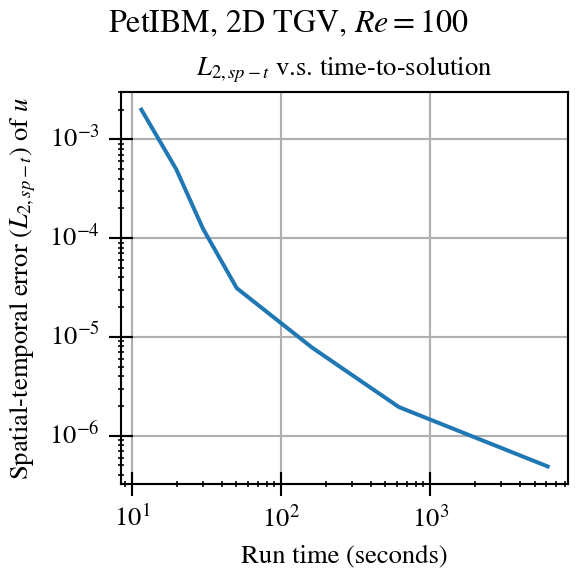
\includegraphics{tgv-2d-re100/petibm/tgv-2d-re100-err-u}%
    \caption[%
        PetIBM, TGV 2D $Re=100$: spatial-temporal error ($L_{2,sp-t}$) of $u$%
    ]{%
        PetIBM, TGV 2D $Re=100$: spatial-temporal error ($L_{2,sp-t}$)  of $u$ versus time-to-solution in seconds%
    }\label{fig:petibm-tgv-spatial-temporal-error}%
\end{figure}
We will be able to compare the time cost to get the desired error with conventional CFD code and with a PINN solver.
The configurations of PetIBM simulations can be found in section \ref{sec:petibm-vv}.
% vim:ft=tex


        \subsection{Result Visualizations}
        \label{sec:pinn-2d-tgv-vis}
        %! TEX root = main.tex

Before we use the cases in the first group for further benchmarking, we examine some results in this section.
We present the training histories and visualizations for the cases with the best, median, and worst $L_{2,sp-t}$ of $u$ velocity.
These cases correspond to $(N_l, N_n, N_{bs}) = (3, 256, 4096)$, $(2, 32, 65536)$, and $(1, 32, 16384)$, respectively.
And their $L_{2,sp-t}$ are $8.3e-3$, $1.4e-1$, and $3.1e-1$.
In the following discussion, we will use the format of $(N_l, N_n, N_{bs})$ to refer to the specific case we are discussing.

\begin{figure}[hbt!]
\centering%
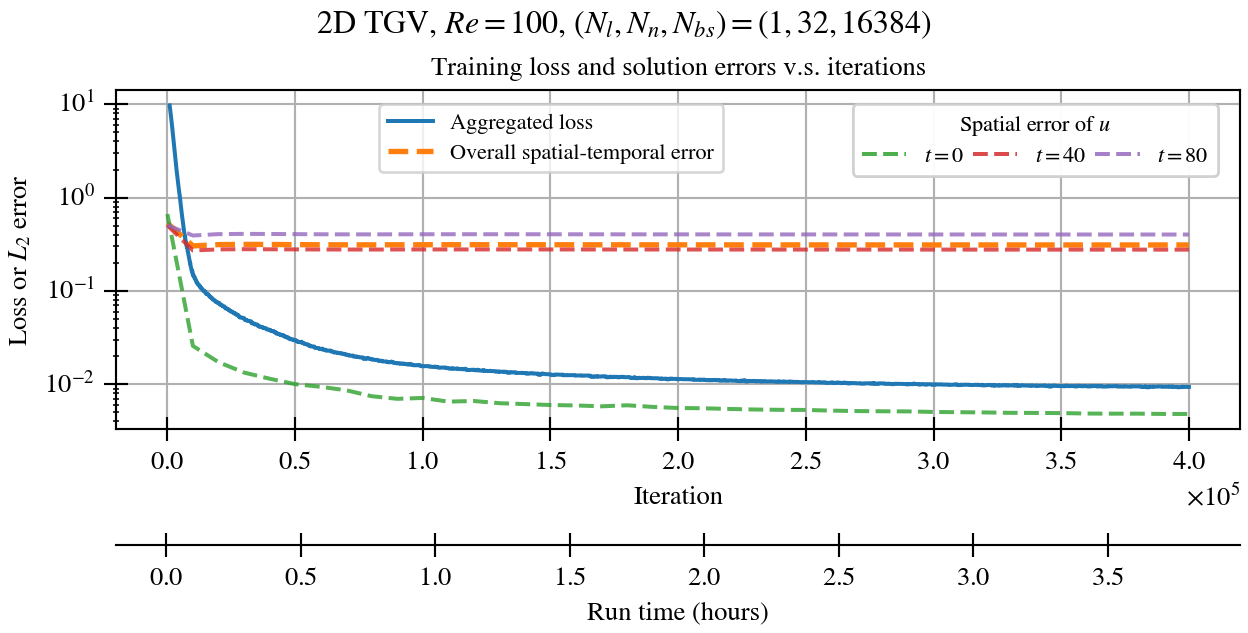
\includegraphics[width=0.9\linewidth]{tgv-2d-re100/training-hist/nl1-nn32-npts16384}%
\caption[%
    PINNs, 2D TGV, $Re=100$: Aggregated loss and $L_2$ errors of $u$ v.s. iterations ($(N_l, N_n, N_{bs})=(1, 32, 16384)$; the worst case)%
]{%
    PINNs, 2D TGV, $Re=100$: Aggregated loss and $L_2$ errors of $u$ v.s. iterations ($(N_l, N_n, N_{bs})$ $=$ $(1, 32, 16384)$; the worst case)%
}\label{fig:nl1-nn32-npts16384-loss-err-hist}%
\end{figure}

\begin{figure}[hbt!]
\centering%
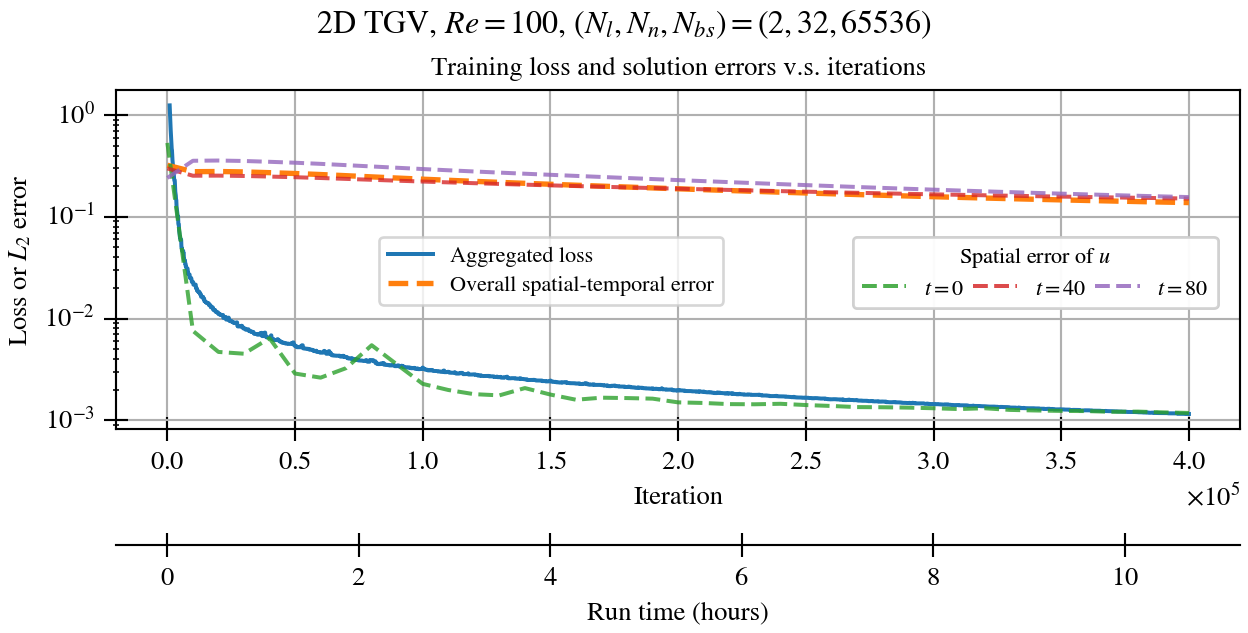
\includegraphics[width=0.9\linewidth]{tgv-2d-re100/training-hist/nl2-nn32-npts65536}%
\caption[%
    PINNs, 2D TGV, $Re=100$: Aggregated loss and $L_2$ errors of $u$ v.s. iterations ($(N_l, N_n, N_{bs})=(2, 32, 65536)$; the median case)%
]{%
    PINNs, 2D TGV, $Re=100$: Aggregated loss and $L_2$ errors of $u$ v.s. iterations ($(N_l, N_n, N_{bs})$ $=$ $(2, 32, 65536)$; the median case)%
}\label{fig:nl2-nn32-npts65536-loss-err-hist}%
\end{figure}

\begin{figure}[hbt!]
\centering%
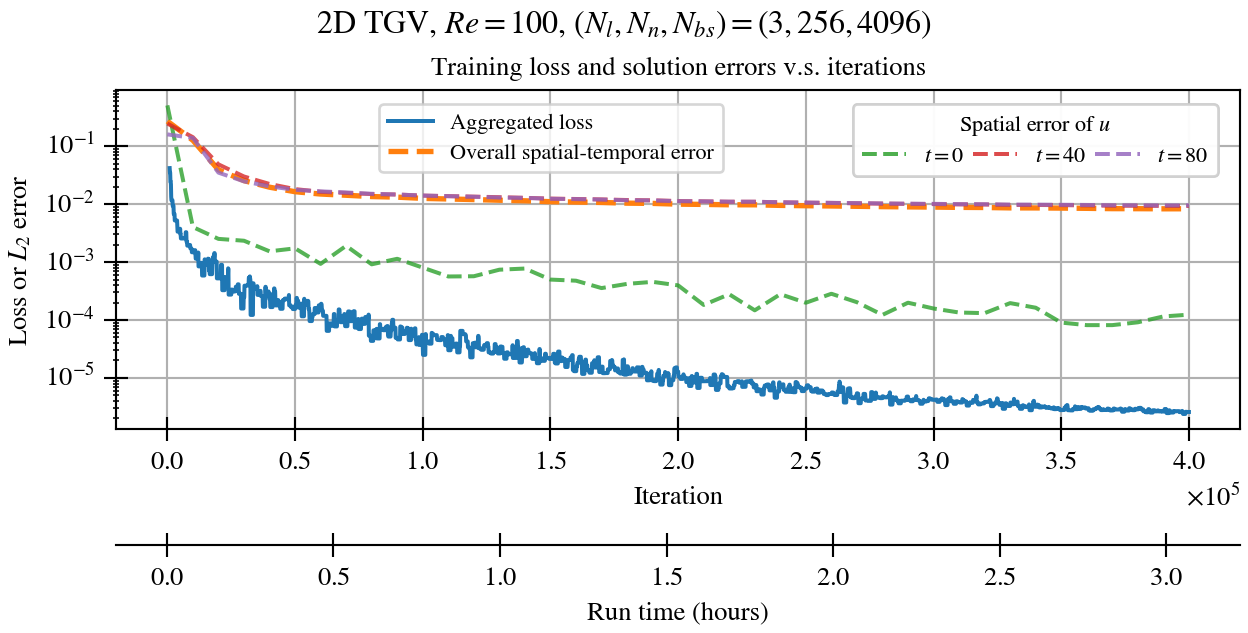
\includegraphics[width=0.9\linewidth]{tgv-2d-re100/training-hist/nl3-nn256-npts4096}%
\caption[%
    PINNs, 2D TGV, $Re=100$: Aggregated loss and $L_2$ errors of $u$ v.s. iterations ($(N_l, N_n, N_{bs})=(3, 256, 4096)$; the best case)%
]{%
    PINNs, 2D TGV, $Re=100$: Aggregated loss and $L_2$ errors of $u$ v.s. iterations ($(N_l, N_n, N_{bs})$ $=$ $(3, 256, 4096)$; the best case)%
}\label{fig:nl3-nn256-npts4096-loss-err-hist}%
\end{figure}

Figures \ref{fig:nl1-nn32-npts16384-loss-err-hist}, \ref{fig:nl2-nn32-npts65536-loss-err-hist}, and \ref{fig:nl3-nn256-npts4096-loss-err-hist} show how the aggregated loss $L_{2,sp-t}$, $L_2@t=0$, $L_2@t=40$, and $L_2@t=80$ for $u$ velocity progressed with training iterations.
A second $x$ axis at the bottom of these figures shows the corresponding run time (in hours).

Only the aggregated loss of $(1, 32, 16384)$ obviously converged, and the other two still show some potential to reach a smaller loss.
However, if we examine the history of $L_{2,sp-t}$, $L_2@t=40$, and $L_2@t=80$, the trends of these errors do not show much potential for improvement.
Especially from the case of $(3, 256, 4096)$, we see that the errors of $u$ does not change significantly after 200,000 iterations.
More training iterations only improve the error at $t=0$.
Note that the solution at $t=0$ is determined by the IC losses only, meaning the correct solution at $t=0$ is given to PINNs.
The solutions of $t=40$ and $t=80$ are mainly affected by PDE losses, and the PINNs do not have correct solutions.
The results shown in these figures mean that PINNs in this benchmark are only able to learn well from where we already provide explicit and correct answers.
PINNs do not perform well on solving the actual PDEs, where the solutions are unknown to them.
And learning well on IC does not help in solving the PDEs.

\begin{figure}[hbt!]
    \centering%
    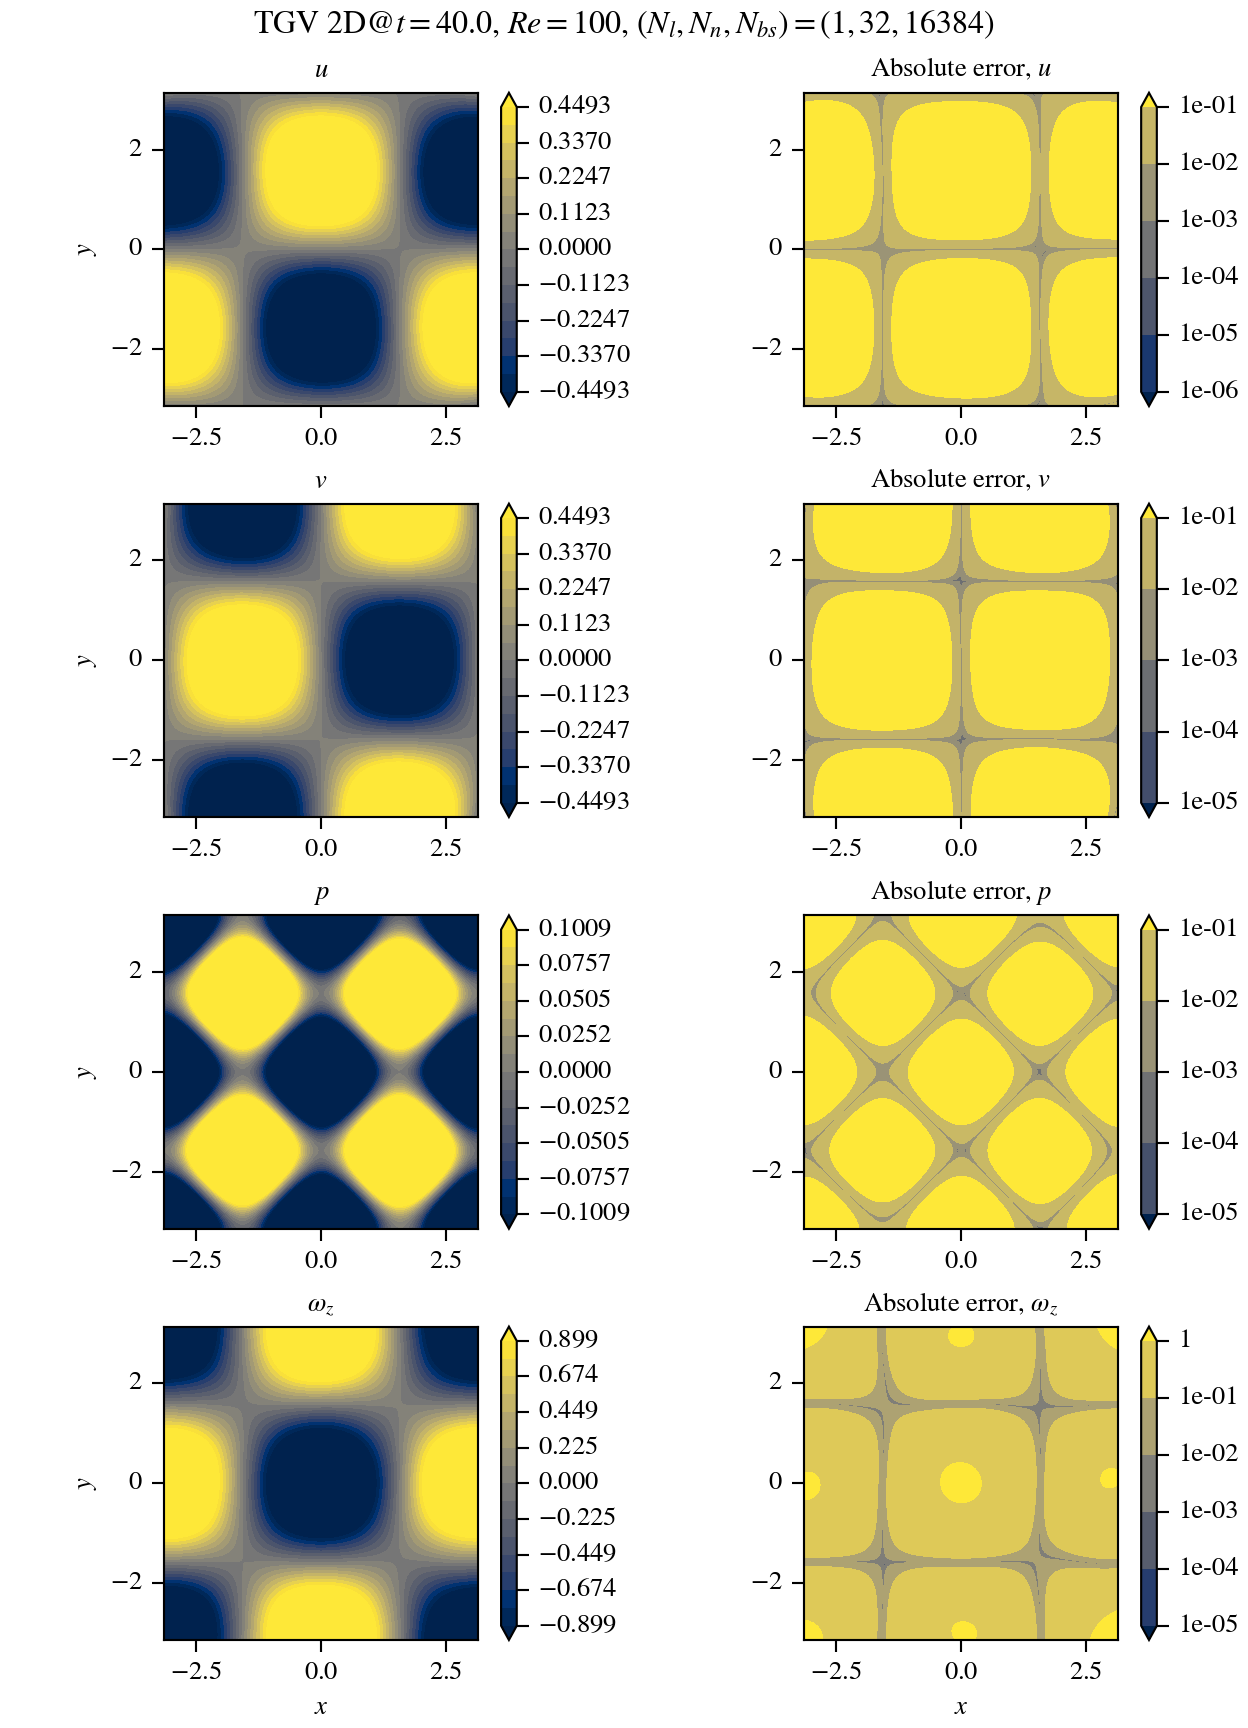
\includegraphics[width=0.9\linewidth]{tgv-2d-re100/contours/nl1-nn32-npts16384-t40.0.png}
    \caption[%
        PINNs, 2D TGV, $Re=100$: Predictions and error contours at $t=40$ ($(N_l, N_n, N_{bs})=(1, 32, 16384)$; the worst case)%
    ]{%
        PINNs, 2D TGV, $Re=100$: Predictions and error contours at $t=40$ ($(N_l, N_n, N_{bs})$ $=$ $(1, 32, 16384)$; the worst case)%
    }
    \label{fig:nl1-nn32-npts16384-t40-contours}
\end{figure}

\begin{figure}[hbt!]
    \centering%
    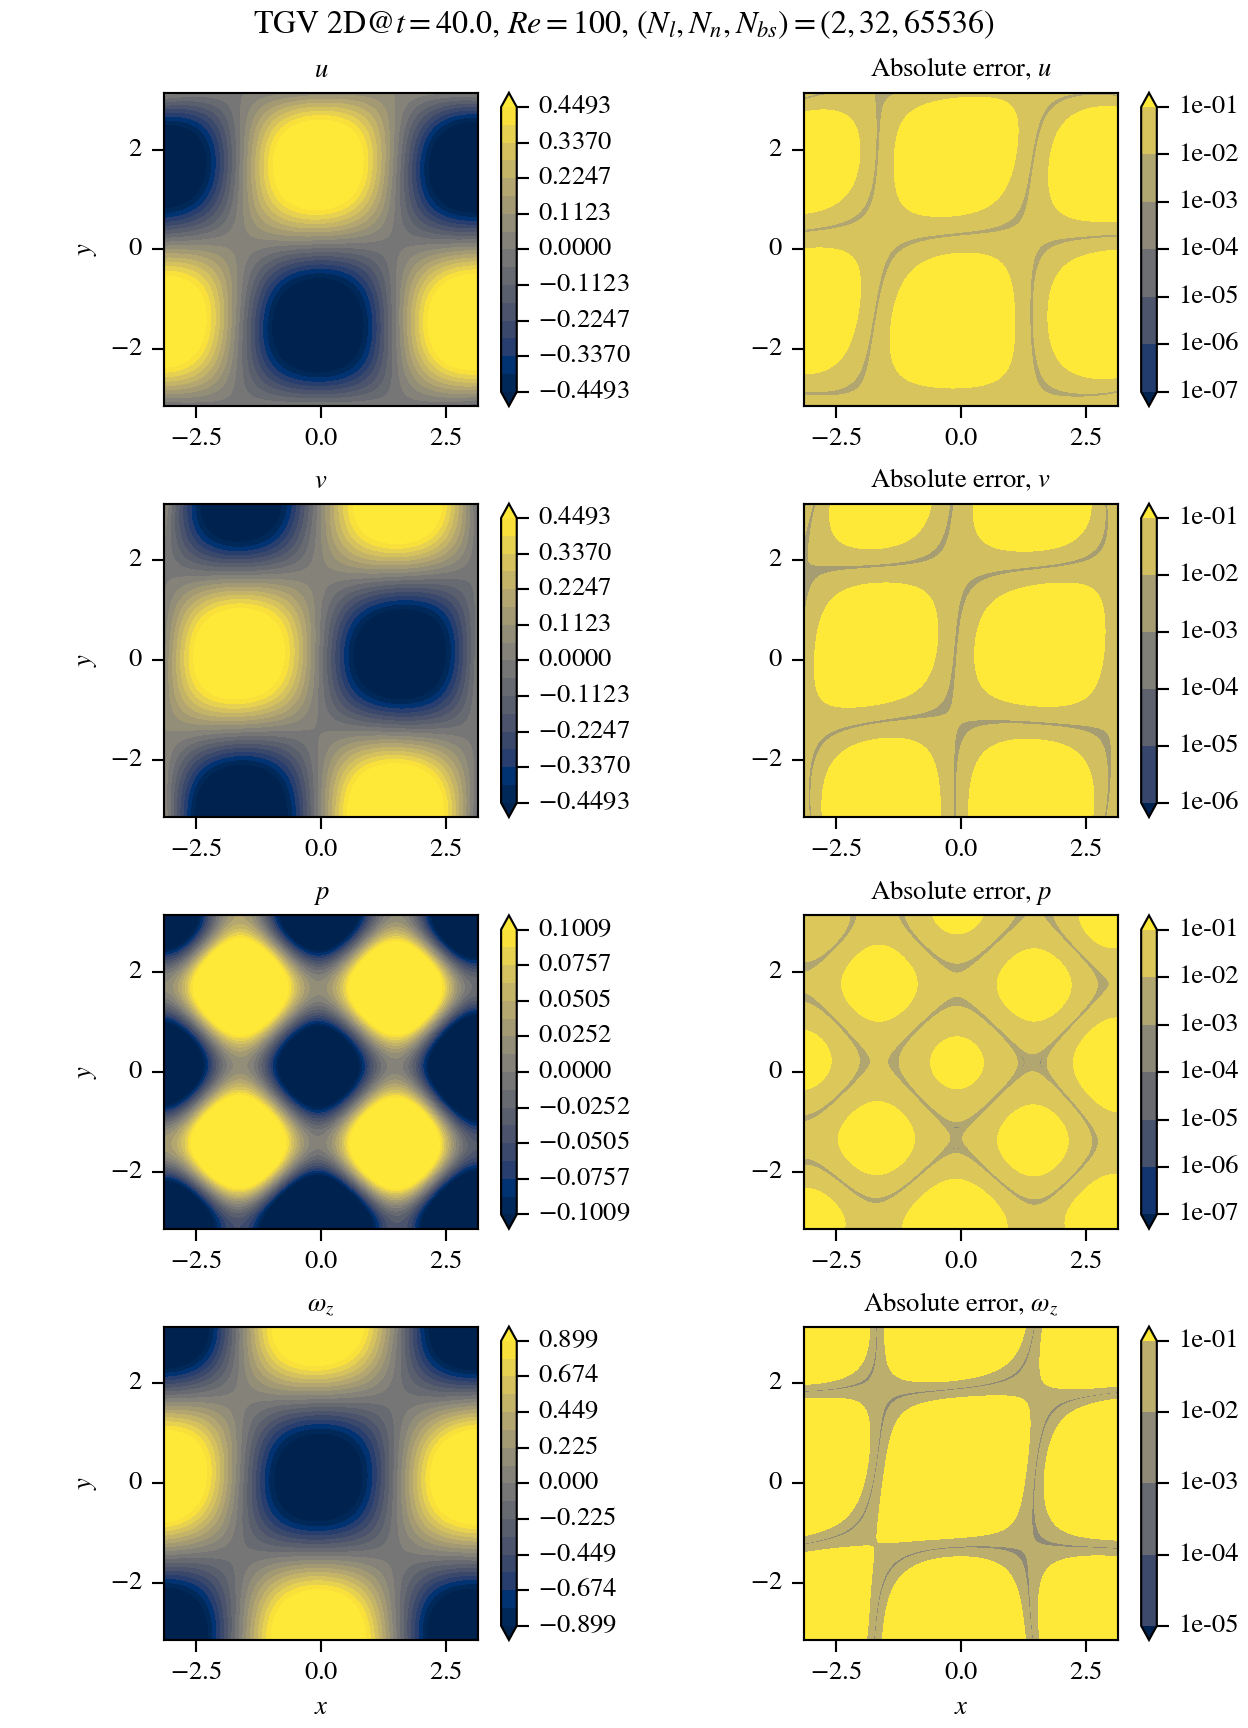
\includegraphics[width=0.9\linewidth]{tgv-2d-re100/contours/nl2-nn32-npts65536-t40.0}
    \caption[%
        PINNs, 2D TGV, $Re=100$: Predictions and error contours at $t=40$ ($(N_l, N_n, N_{bs})=(2, 32, 65536)$; the median case)%
    ]{%
        PINNs, 2D TGV, $Re=100$: Predictions and error contours at $t=40$ ($(N_l, N_n, N_{bs})$ $=$ $(2, 32, 65536)$; the median case)%
    }
    \label{fig:nl2-nn32-npts65536-t40-contours}
\end{figure}

\begin{figure}[hbt!]
    \centering%
    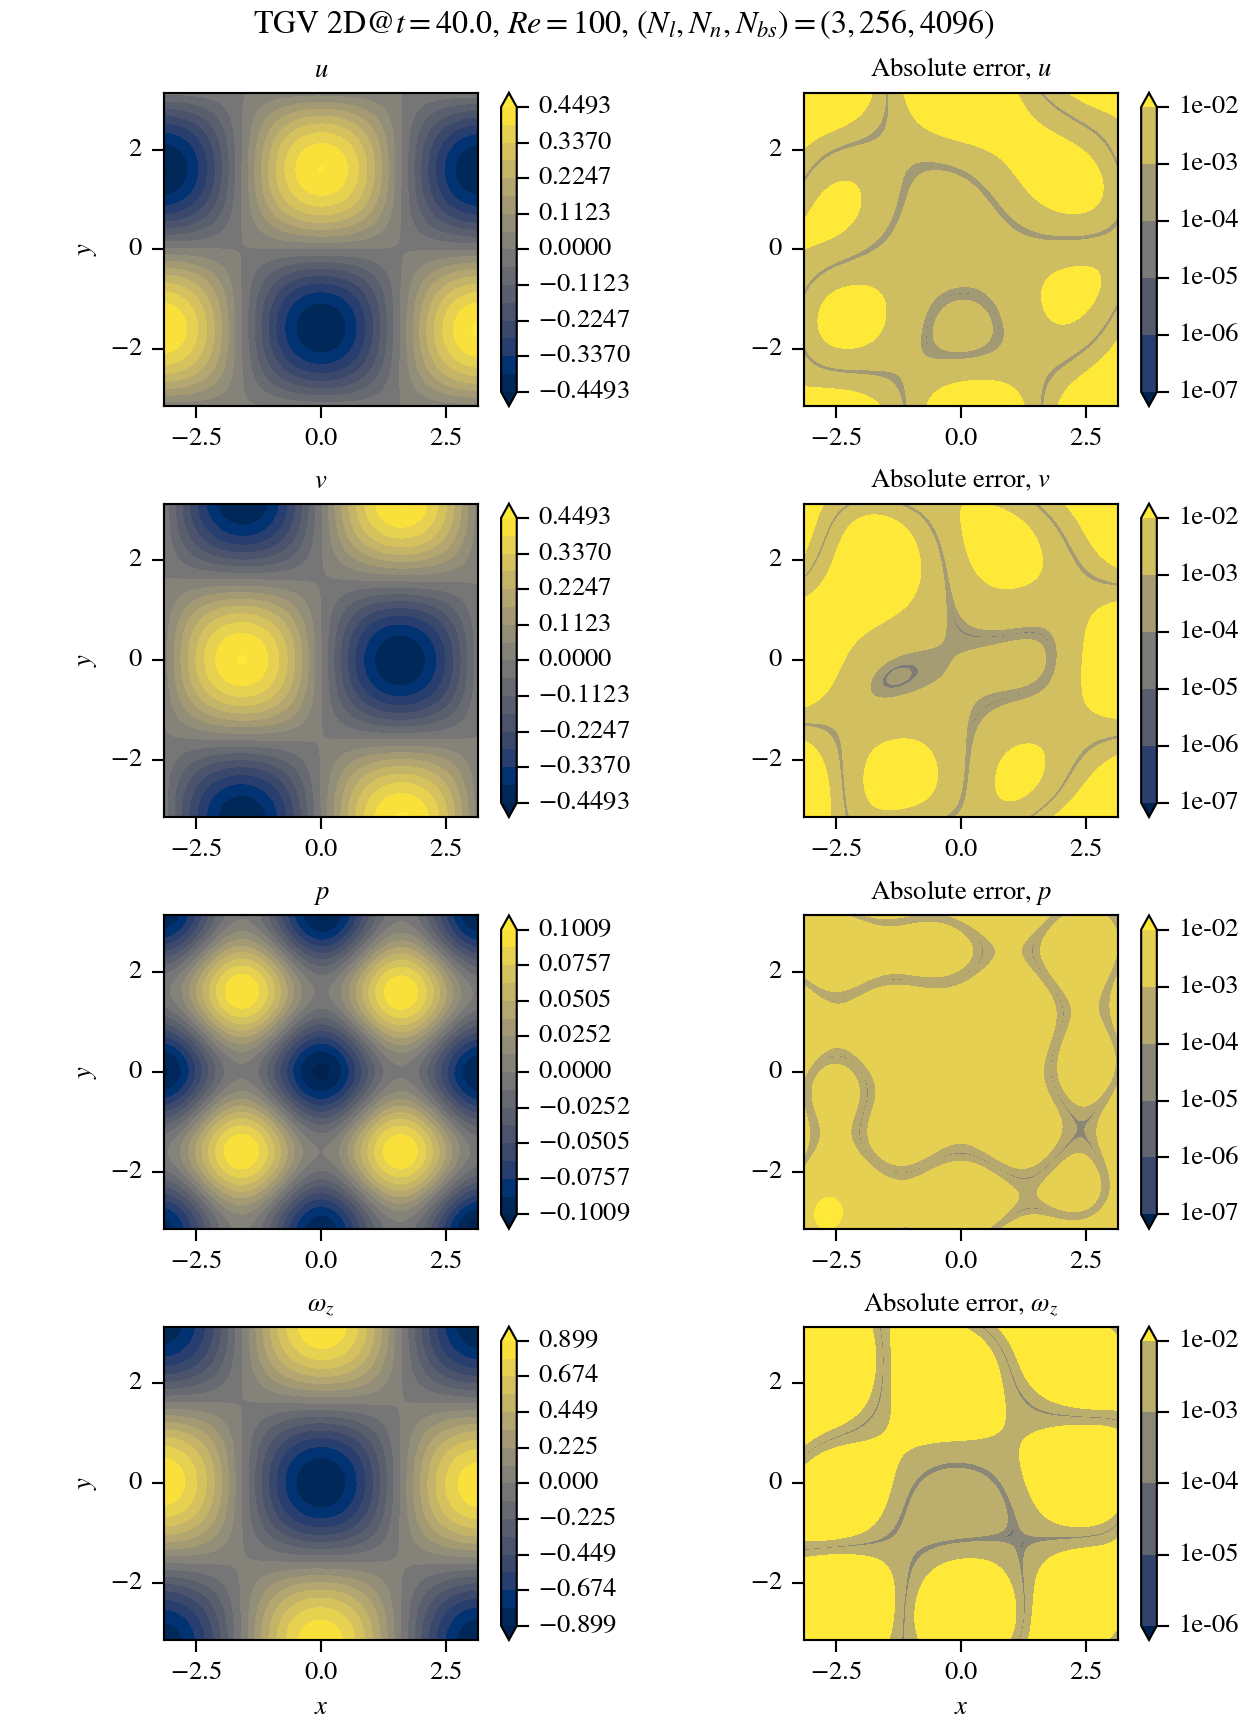
\includegraphics[width=0.9\linewidth]{tgv-2d-re100/contours/nl3-nn256-npts4096-t40.0.png}
    \caption[%
        PINNs, 2D TGV, $Re=100$: Predictions and error contours at $t=40$ ($(N_l, N_n, N_{bs})=(3, 256, 4096)$; the best case)%
    ]{%
        PINNs, 2D TGV, $Re=100$: Predictions and error contours at $t=40$ ($(N_l, N_n, N_{bs})$ $=$ $(3, 256, 4096)$; the best case)%
    }
    \label{fig:nl3-nn256-npts4096-t40-contours}
\end{figure}

If we compare the run times, the case of $(2, 32, 65536)$ took the longest, about 10.5 hours.
The case of $(1, 32, 16384)$ and $(3, 256, 4096)$ took about 3.8 and 3 hours, respectively.
Intuitively speaking, this observation shows that the run times are mainly dominated by the numbers of training points per batch rather than the complexity of a network.

We also compare the final $L_{2,sp-t}$ from the three cases with that in figure \ref{fig:petibm-tgv-spatial-temporal-error}.
While PetIBM was able to achieve an error level of $10^{-3}$ in less than 20 seconds, none of the three PINN cases was able to achieve the same level of error-cost ratio.

Figures \ref{fig:nl1-nn32-npts16384-t40-contours}, \ref{fig:nl2-nn32-npts65536-t40-contours}, and \ref{fig:nl3-nn256-npts4096-t40-contours} show the solution contours at $t=40$ for the three cases.
The color bars' levels are fixed according to the exact solution.
It is obvious that cases with $N_l=1$ and $N_l=2$ only work at where the exact solutions are zero.
The results are not even visually acceptable.
Only the case with $N_l=3$ is able to predict visually acceptable results.
It means both $(1, 16, 15384)$ and $(2, 32, 65536)$ underfit the solution, implying the model complexities are not enough in these two cases.
Later in section \ref{sec:pinn-2d-tgv-model-complexity}, we will see more comparison regarding the run times, model complexity, and the batch sizes.
% vim:ft=tex


        \subsection{Scalability}
        \label{sec:pinn-2d-tgv-scaling}
        %! TEX root = main.tex

In this section, we are interested in the scalability of PINNs.
In the weak scaling tests, we scaled $(2, 32, 8192)$ and $(3, 128, 8192)$ with 1, 2, 4, and 8 GPUs. 
As for the strong scaling tests, we scaled $(2, 32, 65536)$ and $(3, 128, 65536)$ with 1, 2, 4, and 8 GPUs. 
We will use an expression of $(N_l, N_n, N_{bs})\times N_{gpu}$ to denote how many GPUs are used and how many training points per batch on each GPU.
On the other, an expression of $(N_l, N_n, N_{bs}\times N_{gpu})$ denotes a case running on only one GPU but has $N_{bs}\times N_{gpu}$ training points per batch.

Figures \ref{fig:nl2-nn32-npts8192-weak-scaling} and \ref{fig:nl3-nn128-npts8192-weak-scaling} show the results of weak scaling tests.
These figures show the losses and errors of $u$ versus iterations on the left $y$-axis.
And for the other $y$-axis, we have the run times in hours versus iterations.

\begin{figure}[hbt!]
    \centering%
    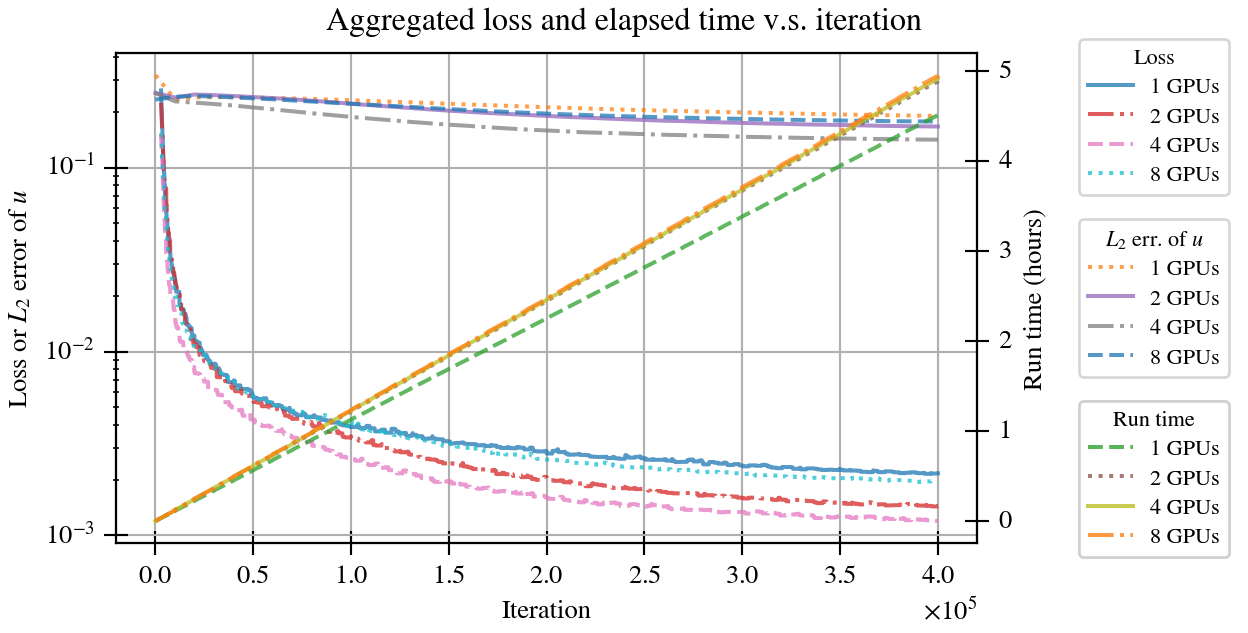
\includegraphics[width=0.9\linewidth]{tgv-2d-re100/scaling-tests/nl2-nn32-npts8192-weak-scaling.png}
    \caption[%
        Weak scaling: aggregated loss and run time v.s. iteration ($(N_l, N_n, N_{bs})$ $=$ $(2, 32, 8192)$)%
    ]{%
        Weak scaling: aggregated loss and run time v.s. iteration ($(N_l, N_n, N_{bs})$ $=$ $(2, 32, 8192)$)%
    }\label{fig:nl2-nn32-npts8192-weak-scaling}
\end{figure}

\begin{figure}[hbt!]
    \centering%
    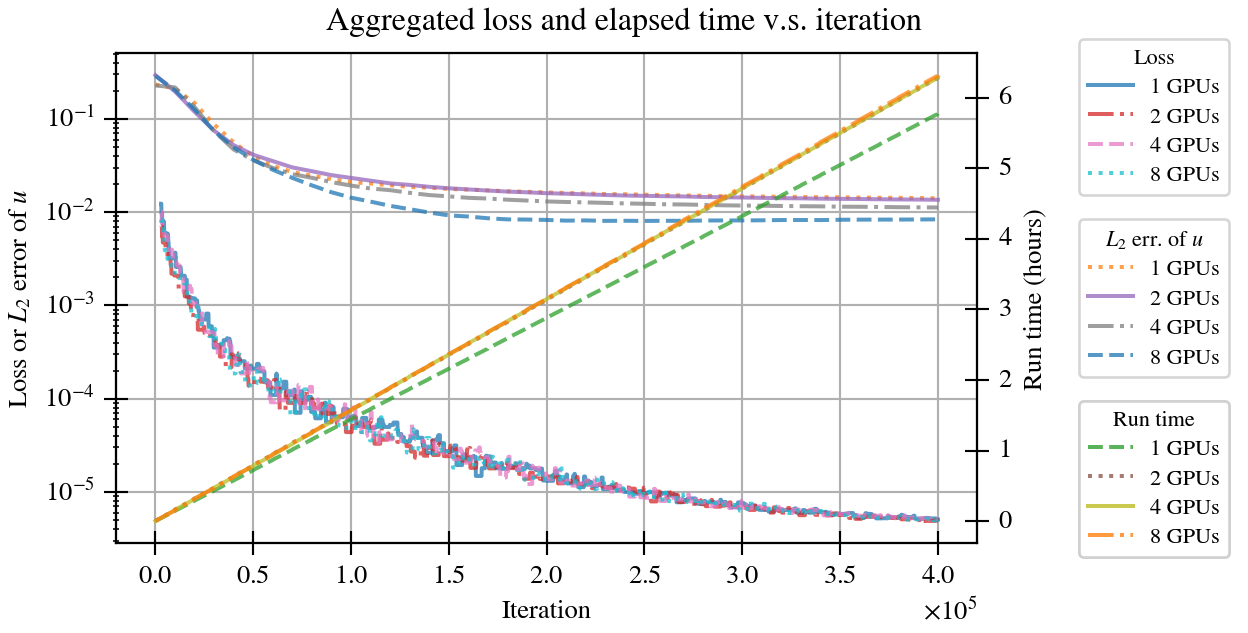
\includegraphics[width=0.9\linewidth]{tgv-2d-re100/scaling-tests/nl3-nn128-npts8192-weak-scaling.png}
    \caption[%
        Weak scaling: aggregated loss and run time v.s. iteration ($(N_l, N_n, N_{bs})$ $=$ $(3, 128, 8192)$)%
    ]{%
        Weak scaling: aggregated loss and run time v.s. iteration ($(N_l, N_n, N_{bs})$ $=$ $(3, 128, 8192)$)%
    }\label{fig:nl3-nn128-npts8192-weak-scaling}
\end{figure}

In weak scaling, because each GPU has the same amount of work loading, the run time versus iterations should be the same for different cases.
From figure \ref{fig:nl2-nn32-npts8192-weak-scaling} and \ref{fig:nl3-nn128-npts8192-weak-scaling}, we found that, except for the 1-GPU cases, cases with other GPUs match each other.
The reason that 1-GPU cases show different results may be that it does not have the latency overhead due to exchanging with other GPUs.

We further checked the losses and error histories and considered no significant difference between using different numbers of GPUs.
Note that while lines do not overlap on the figures, quantitatively speaking, the difference in the orders of magnitude is minor, as we will see in table \ref{table:weak-scaling-perf}. 

Theoretically, $(N_l, N_n, N_{bs})\times N_{gpu}$ is expected to equal to $(N_l, N_n, N_{bs}\times N_{gpu})$ in terms of losses and errors.
So the difference between using a different number of GPUs should be similar to the effect of using a different number of training points per batch on one GPU.
We will examine the effect of different $N_{bs}$ in section \ref{sec:pinn-2d-tgv-model-complexity}.
Instead, here we would like to check if it is true that $(N_l, N_n, N_{bs})\times N_{gpu}$ is equivalent to $(N_l, N_n, N_{bs}\times N_{gpu})$.
Figure \ref{fig:nl2-nn32-npts8192-multi-singl-gpus} shows the comparisons between $(2, 32, 8192)\times N_{gpu}$ and $(2, 32, 8192\times N_{gpu})$.
And figure \ref{fig:nl3-nn128-npts8192-multi-singl-gpus} shows the same comparisons between $(3, 128, 8192)\times N_{gpu}$ and $(3, 128, 8192\times N_{gpu})$.

\begin{figure}[hbt!]
    \centering%
    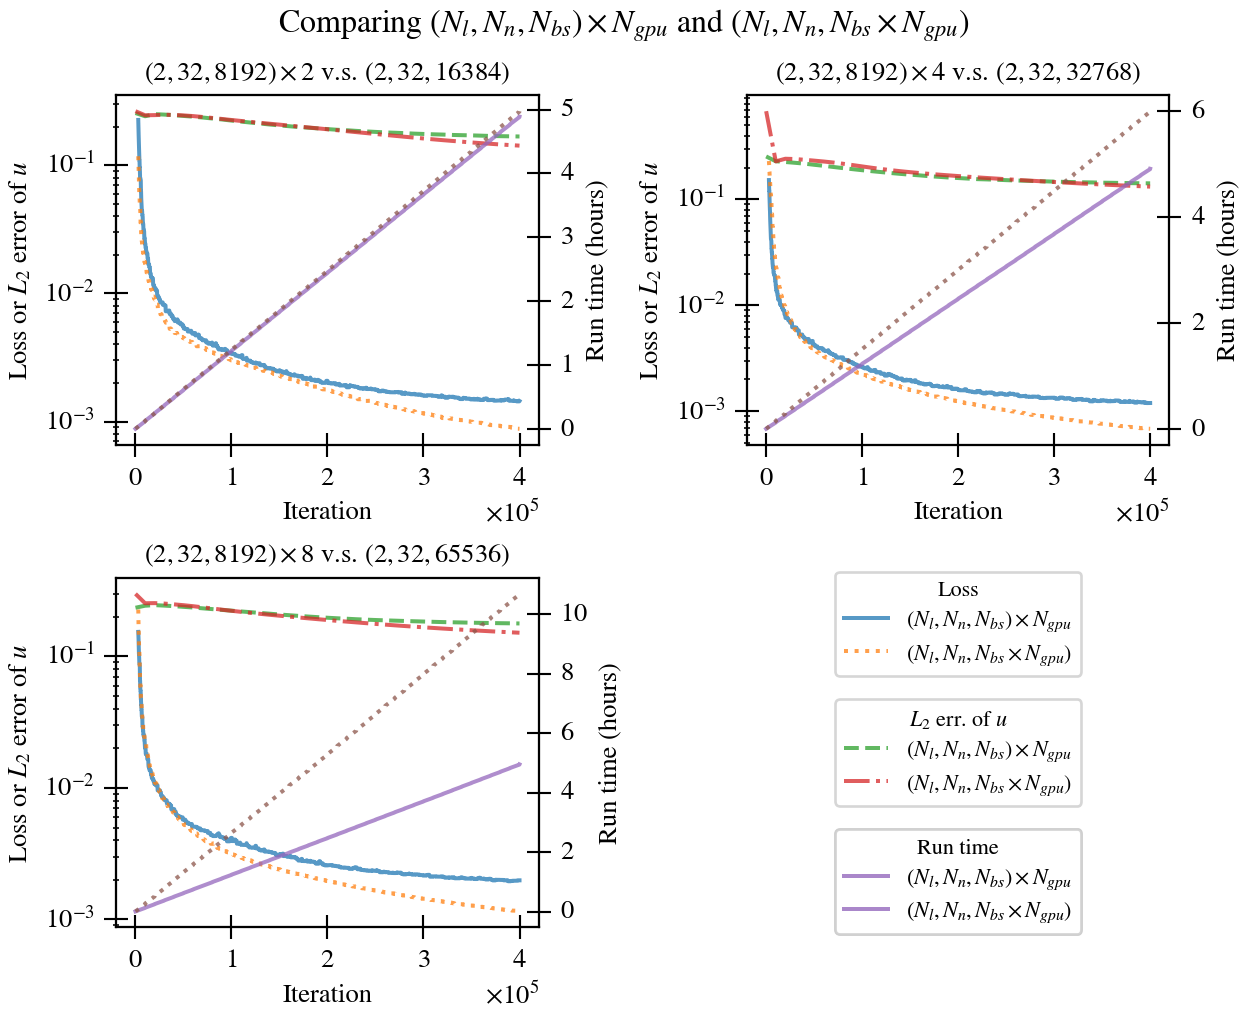
\includegraphics[width=0.9\linewidth]{tgv-2d-re100/scaling-tests/nl2-nn32-npts8192-multi-singl-gpus.png}
    \caption[%
        Comparing multi-GPU and single-GPU cases ($(N_l, N_n)$ $=$ $(2, 32)$)%
    ]{%
        Comparing multi-GPU and single-GPU cases ($(N_l, N_n)$ $=$ $(2, 32)$)%
    }\label{fig:nl2-nn32-npts8192-multi-singl-gpus}
\end{figure}

\begin{figure}[hbt!]
    \centering%
    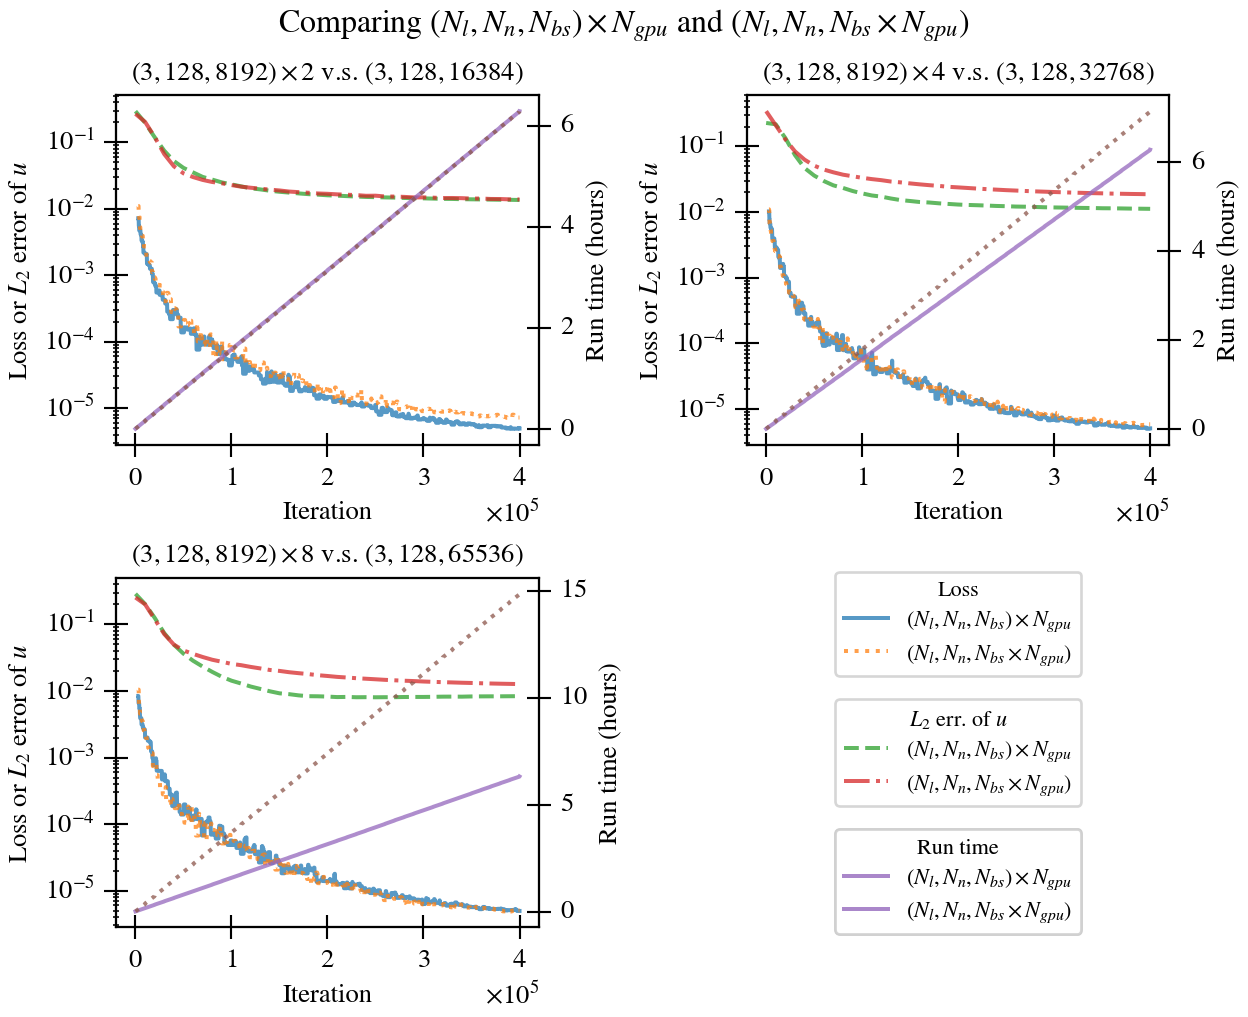
\includegraphics[width=0.9\linewidth]{tgv-2d-re100/scaling-tests/nl3-nn128-npts8192-multi-singl-gpus.png}
    \caption[%
        Comparing multi-GPU and single-GPU cases ($(N_l, N_n)$ $=$ $(3, 128)$)%
    ]{%
        Comparing multi-GPU and single-GPU cases ($(N_l, N_n)$ $=$ $(3, 128)$)%
    }\label{fig:nl3-nn128-npts8192-multi-singl-gpus}
\end{figure}

In these figures, it is expected that the run times are different and that the losses and errors are similar.
However, though losses and errors show similar trends between $(N_l, N_n, N_{bs})\times N_{gpu}$ and $(N_l, N_n, N_{bs}\times N_{gpu})$, visible differences exist.
In $(N_l, N_n)=(2, 32)$, losses stop improving earlier for multi-GPU cases, and multi-GPU cases have slightly worse errors.
On the other hand, for $(N_l, N_n)=(3, 128)$, the multi-GPU cases in general have better errors, though the loss histories do not show a noticeable difference.
The reason is unknown to us at this point.
The observation shows that $(N_l, N_n, N_{bs})\times N_{gpu}$ and $(N_l, N_n, N_{bs}\times N_{gpu})$ are not necessarily the same.
Nevertheless, we believe the differences are quantitatively minor if we consider their orders of magnitude.

\begin{table}[hbt!]
\centering
\singlespacing
\caption[
    PINNs, 2D TGV, $Re=100$: weak scaling performance for $(N_l, N_n, N_{bs})=(2, 32, 8192)$ and $(3, 128, 8192)$
]{
    Weak scaling performance for $(N_l, N_n, N_{bs})$ $=$ $(2, 32, 8192)$ and $(3, 128, 8192)$.%
    Time costs denote the wall time required to finish 400k training iterations in hours.%
    Efficiency here stands for weak scaling efficiency in $\%$.%
    The aggregated losses are those at the last iteration.%
    The $L_{2, sp-t}$ errors were the overall spatial-temporal errors at the last training iteration.%
}
\label{table:weak-scaling-perf}
\begin{tabular}{lcccccccc}
\toprule
 & \multicolumn{4}{c}{(2, 32, 8192)} & \multicolumn{4}{c}{(3, 128, 8192)} \\
\cmidrule(rl){2-5} \cmidrule(rl){6-9}
\multicolumn{1}{r}{GPUs} & 1 & 2 & 4 & 8 & 1 & 2 & 4 & 8 \\
\midrule
Time cost &  4.51 &  4.89 &  4.92 &  4.95 &  5.77 &  6.28 &  6.29 &  6.32 \\
\addlinespace
Efficiency & 100 & 92 & 92 & 91 & 100 & 92 & 92 & 91 \\
\addlinespace
Loss & 2.2e-03 & 1.5e-03 & 1.2e-03 & 2.1e-03 & 6.7e-06 & 5.3e-06 & 5.5e-06 & 5.3e-06 \\
\addlinespace
$L_{2,sp-t}$, $u$ & 1.9e-01 & 1.5e-01 & 1.2e-01 & 1.7e-01 & 1.3e-02 & 1.3e-02 & 1.0e-02 & 8.9e-03 \\
\addlinespace
$L_{2,sp-t}$, $v$ & 1.9e-01 & 1.5e-01 & 1.3e-01 & 1.8e-01 & 1.1e-02 & 1.2e-02 & 1.1e-02 & 9.6e-03 \\
\bottomrule
\end{tabular}
\end{table}


The quantitative results are listed in table \ref{table:weak-scaling-perf}.
The weak-scaling efficiencies are all above $90\%$.
The losses and errors are close in terms of the orders of magnitude.
PINNs generally have good weak-scaling if we define the workload using $N_{bs}$.
During training, each GPU calculates the gradients $\nabla_{\Theta} r(\Theta)$ independently, and then each training iteration only needs one reduction operation to calculate the averaged gradients across all GPUs.
A good weak scaling is thus expected.

Lastly, we examined the strong scaling.
Figure \ref{fig:nl2-nn32-npts65536-strong-scaling} shows the strong scaling results of $(2, 32, 65535)\times 1$, $(2, 32, 32768)\times 2$, $(2, 32, 16384)\times 4$, and $(2, 32, 8192)\times 8$.
Figure \ref{fig:nl3-nn128-npts65536-strong-scaling} shows the similar strong scaling tests for $(N_l, N_n)=(3, 128)$.
Quantitative results are listed in table \ref{table:strong-scaling-perf}. 

\begin{figure}[hbt!]
    \centering%
    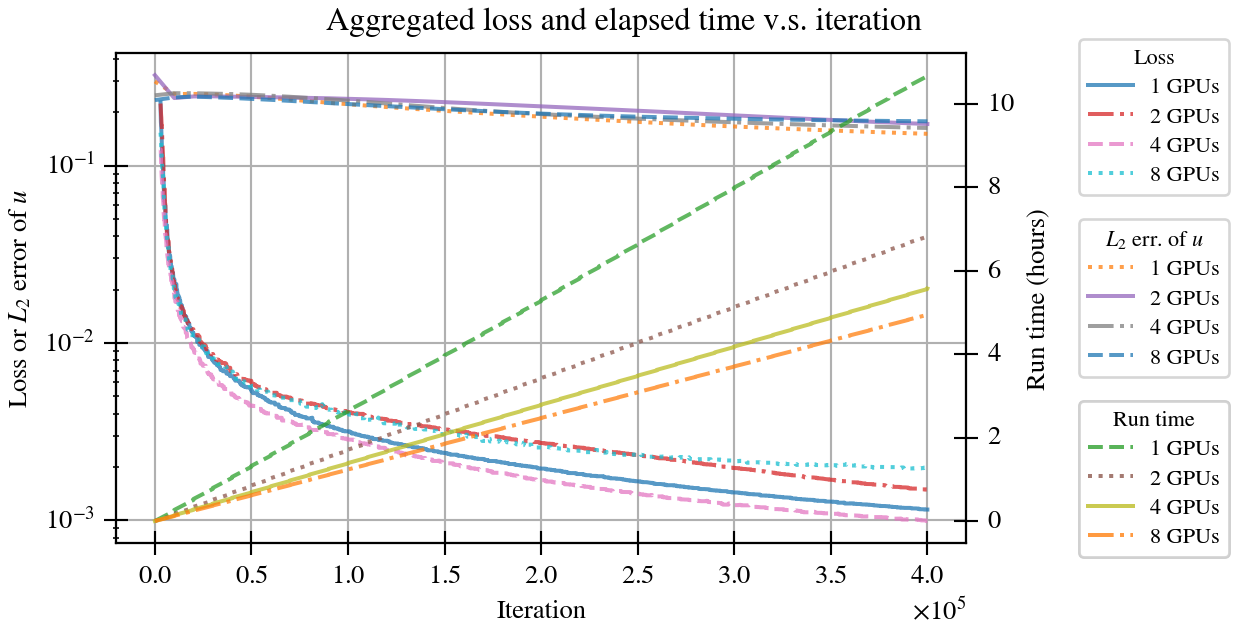
\includegraphics[width=0.9\linewidth]{tgv-2d-re100/scaling-tests/nl2-nn32-npts65536-strong-scaling.png}
    \caption[%
        Strong-scaling: aggregated loss and run time v.s. iteration ($(N_l, N_n, N_{bs})$ $=$ $(2, 32, 65535)$)%
    ]{%
        Strong-scaling: aggregated loss and run time v.s. iteration ($(N_l, N_n, N_{bs})$ $=$ $(2, 32, 65535)$)%
    }\label{fig:nl2-nn32-npts65536-strong-scaling}
\end{figure}

\begin{figure}[hbt!]
    \centering%
    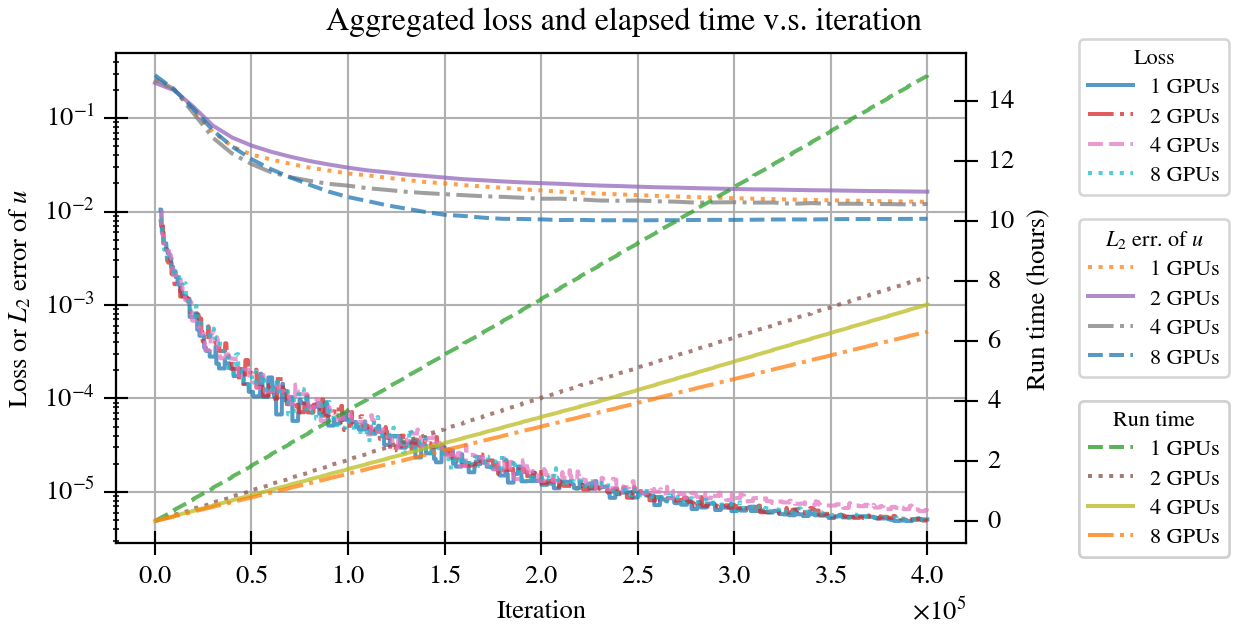
\includegraphics[width=0.9\linewidth]{tgv-2d-re100/scaling-tests/nl3-nn128-npts65536-strong-scaling.png}
    \caption[%
        Strong-scaling: aggregated loss and run time v.s. iteration ($(N_l, N_n, N_{bs})$ $=$ $(3, 128, 65535)$)%
    ]{%
        Strong-scaling: aggregated loss and run time v.s. iteration ($(N_l, N_n, N_{bs})$ $=$ $(3, 128, 65535)$)%
    }\label{fig:nl3-nn128-npts65536-strong-scaling}
\end{figure}

Theoretically, a good strong scaling result should show similar losses and errors.
Figures \ref{fig:nl2-nn32-npts65536-strong-scaling} and \ref{fig:nl3-nn128-npts65536-strong-scaling}, instead, exhibit some differences.
However, if we consider their orders of magnitude, we consider the differences minor.
This claim can be examined from table \ref{table:strong-scaling-perf}.
On the other hand, the results show deteriorating strong scaling efficiencies.
The worse strong scaling is caused by only dividing the training points across GPUs, while the model itself is not divided.  
The model complexity also contributes to the work loading.
We do not have a clear way to divide a model and distribute the work loading across GPUs.
Neither do we have means to exclude the model's contribution to the work loading and correctly calculate the strong scaling efficiencies and speedups.
Lacking these knowledges limited our investigation into the strong scaling of PINNs.

\begin{table}[hbt!]
\centering
\singlespacing
\caption[
    PINNs, 2D TGV, $Re=100$: strong scaling performance for $(N_l$, $N_n$, $N_{bs})$ $=$ $(2$, $32$, $65536)$ and $(3$, $128$, $65536)$
]{
    Strong scaling performance for $(N_l$, $N_n$, $N_{bs})$ $=$ $(2$, $32$, $65536)$ and $(3$, $128$, $65536)$.%
    Time costs denote the wall time required to finish 400k training iterations in hours.%
    Efficiency here stands for strong scaling efficiency in $\%$.%
    The aggregated losses were those at the last iteration.%
    The $L_{2,sp-t}$ errors were the overall spatial-temporal errors at the last training iteration.%
}
\label{table:strong-scaling-perf}
\begin{tabular}{lcccccccc}
\toprule
 & \multicolumn{4}{c}{(2, 32, 65536)} & \multicolumn{4}{c}{(3, 128, 65536)} \\
\cmidrule(rl){2-5} \cmidrule(rl){6-9}
\multicolumn{1}{r}{GPUs} & 1 & 2 & 4 & 8 & 1 & 2 & 4 & 8 \\
\midrule
Time cost & 10.69 &  6.82 &  5.57 &  4.95 & 14.79 &  8.12 &  7.23 &  6.32 \\
\addlinespace
Speedup & 1.0x & 1.6x & 1.9x & 2.2x & 1.0x & 1.8x & 2.0x & 2.3x \\
\addlinespace
Efficiency & 100 & 78 & 48 & 27 & 100 & 91 & 51 & 29 \\
\addlinespace
Loss & 1.2e-03 & 1.5e-03 & 1.0e-03 & 2.1e-03 & 5.1e-06 & 5.2e-06 & 6.7e-06 & 5.3e-06 \\
\addlinespace
$L_{2,sp-t}$, $u$ & 1.4e-01 & 1.6e-01 & 1.5e-01 & 1.7e-01 & 1.1e-02 & 1.6e-02 & 1.2e-02 & 8.9e-03 \\
\addlinespace
$L_{2,sp-t}$, $v$ & 1.4e-01 & 1.6e-01 & 1.5e-01 & 1.8e-01 & 1.0e-02 & 1.7e-02 & 1.2e-02 & 9.6e-03 \\
\bottomrule
\end{tabular}
\end{table}

% vim:ft=tex

        \subsection{Aggregate Loss and Prediction Accuracy}
        \label{sec:pinn-2d-tgv-loss-vs-accuracy}
        %! TEX root = main.tex
One particular question we would like to investigate is the relationship between training loss and the actual prediction errors or accuracy.
As we have seen from the previous section, further training in many cases only reduces the IC losses, while the PDE losses already converged.
Reductions in IC losses, though they improve the prediction error of the solution at $t=0$, do not help the overall spatial-temporal $L_{2,sp-t}$ at all.
This implies the training loss may not reflect the models' prediction capabilities.
If true, then the aggregated loss is not a sufficient indicator to monitor the training progress.
Also, given a known aggregated loss and error, we may not able to predict how much loss we need to further reduce and achieve a desired error level.
We would hence like to investigate the relationship between the aggregated loss and the overall spatial-temporal errors.

Figure \ref{fig:tgv2d-re100-err-vs-loss} shows the $L_{2,sp-t}$ of all cases.
The $x$-axis represents the square roots of aggregate losses, and the $y$-axis is $L_{2,sp-t}$ of $u$ and $v$.
For each case, $u$ and $v$ are separate dots in the figure.
The figure uses the square roots of aggregate losses because losses are defined as the sum of residuals' squares.
See equation \eqref{eq:residual-norms}

\begin{figure}[hbt!]
    \centering%
    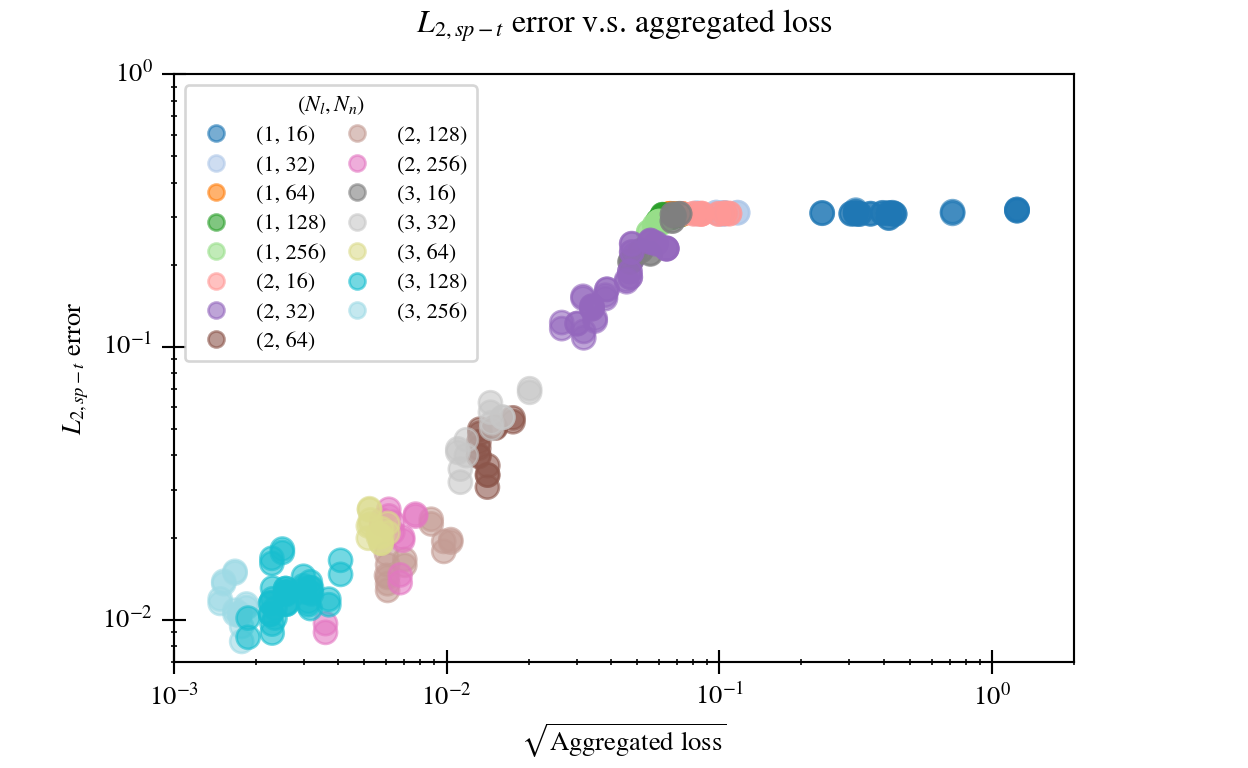
\includegraphics[width=0.9\linewidth]{tgv-2d-re100/err-vs-loss/err-loss.png}
    \caption[%
        PINNs, 2D TGV, $Re=100$: $L_{2,sp-t}$ error v.s. aggregated loss%
    ]{%
        PINNs, 2D TGV, $Re=100$: $L_{2,sp-t}$ error v.s. aggregated loss. %
        $L_{2,sp-t}$ errors for $u$ and $v$ from the same case are separate data points in the figure.
    }
    \label{fig:tgv2d-re100-err-vs-loss}
\end{figure}

From the figure, the first observation is the flat region in the top-right corner.
These cases are mainly those with only one hidden layer, implying that one hidden layer may not be enough to approximate the solutions of the Navier-Stokes equations.

Although the relationship is approximately linear in the middle range, the data points become more scattered in the bottom-left corner, and a similar loss level has a wider range of possible $L_{2,sp-t}$.
Given the observed trends, it is reasonable to suspect that, if we had more data further to the left of this figure, the possible $L_{2,sp-t}$ corresponding to a loss level may have a wider and wider scatter, meaning it is more difficult to predict the solution accuracy for a given training loss.

In addition, we suspect that using adaptive loss weighting like annealing loss aggregation may exacerbate the problem.
As each loss term's weight is updated according to the ratio of characteristic gradient magnitudes, it is likely that two iterations will have the same level of aggregated losses but have different prediction accuracies. 
This observation somehow hurts the predictability of PINNs.
Especially when dealing with real-world problems where we don't have exact solutions to calculate the errors, the losses may be the only indicator for us to estimate a model's prediction capability.
If lowering the loss does not improve the prediction accuracy, we have no means to know if training should keep going.
% vim:ft=tex


        \subsection{Model Complexity, Batch sizes, and Time Costs}
        \label{sec:pinn-2d-tgv-model-complexity}
        %! TEX root = main.tex

In conventional numerical methods, the degrees of freedom (i.e., the numbers of model parameters) reflect the model complexity.
And given a numerical method and a model complexity, the workload, time cost, and accuracy are theoretically predictable.
In PINNs, the number of model parameters also determines the model complexity.
However, even with a specific PINN implementation, model complexity may not be the only factor determining the time cost and the accuracy.
The number of training points per batch ($N_{bs}$) apparently also influences the time cost.
One interesting question is whether $N_{bs}$ affects the prediction accuracy or errors.
If yes, then how to choose a proper $N_{bs}$ is a follow-up question. 
If no, it means the time cost does not reflect the PINN methods' performance.
In this section, we would like to examine the relationship between model complexity, batch sizes, error levels, and the time costs.

We first visualize the $L_{2,sp-t}$ errors of $u$ for all cases in figure \ref{fig:tgv2d-re100-err-vs-arch}.
\begin{figure}[hbt!]
    \centering%
    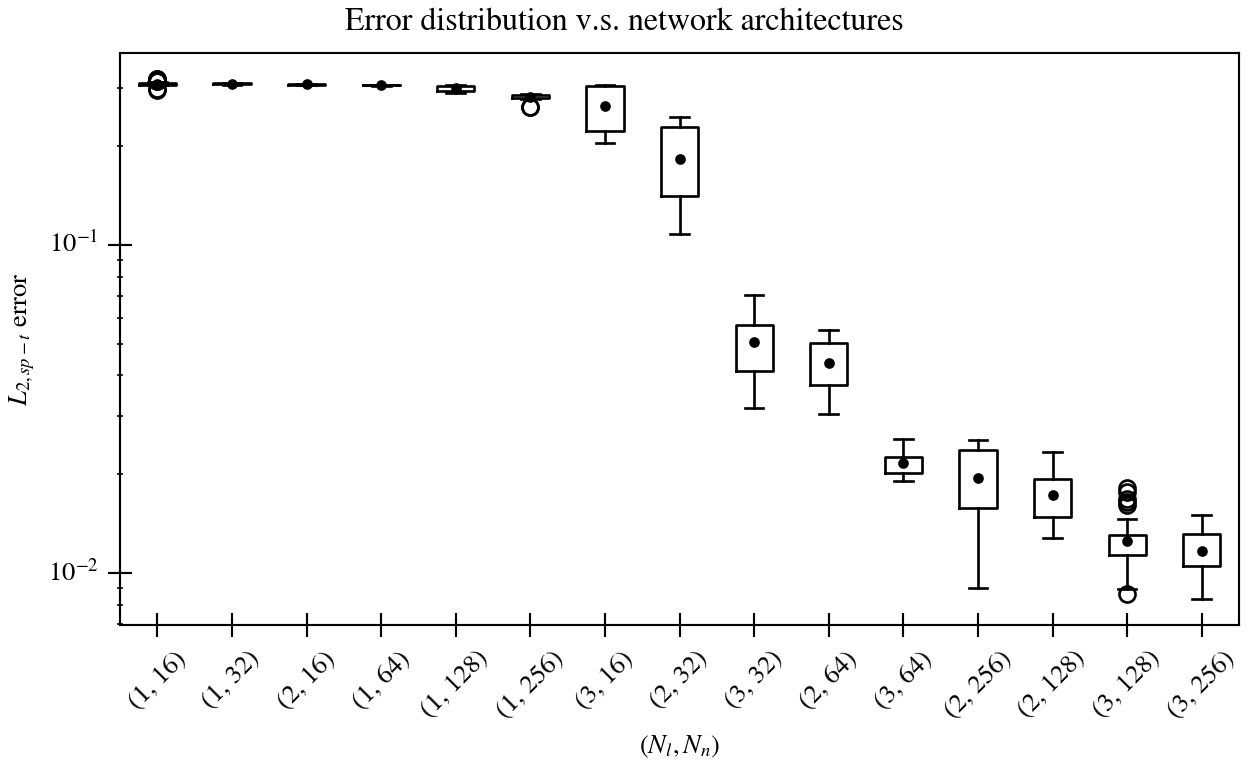
\includegraphics[width=0.95\linewidth]{tgv-2d-re100/err-vs-model-complexity/err-arch-boxplot}
    \caption[%
        PINNs, 2D TGV, $Re=100$: $L_{2,sp-t}$ error v.s. network architecture%
    ]{%
        PINNs, 2D TGV, $Re=100$: $L_{2,sp-t}$ error v.s. network architecture%
    }
    \label{fig:tgv2d-re100-err-vs-arch}
\end{figure}
The $y$-axis is $L_{2,sp-t}$, and $x$-axis denotes the network architectures $(N_l, N_n)$.
The architectures are sorted by their error magnitudes from left to right.
The box plot of each architecture represents the error distributions of different $N_{bs}$ with the same architecture.
We hope this figure can shed some light on how $N_l$, $N_n$, and $N_{bs}$ influence the error levels.
The figure shows that, when $N_l < 2$ or $N_n < 32$, the errors remain at the same level, and $N_{bs}$ does not have any influence.
This may indicate these models are too simple and always underfit the PDEs.
Once the model complexity reaches a certain level, increasing both $N_n$ and $N_l$ helps lower the error levels.
Also, $N_{bs}$ starts to have an effect in these cases.
Nevertheless, if we consider the orders of magnitudes, quantitatively speaking, we don't consider that $N_{bs}$ has a strong impact on the accuracy.
As seen from the figure, model complexity still dominates the error levels. 

It is unclear from figure \ref{fig:tgv2d-re100-err-vs-arch} whether increasing $N_l$ or $N_n$ has a stronger impact on the error levels.
For example, if we are to improve the error level of $(N_l$, $N_n)$ $=$ $(2$, $32)$, both $(2$, $64)$ and $(3$, $32)$ give us similar improvement.
Or, if we are to improve the error of $(2$, $64)$, both $(2$, $128)$ and $(3$, $64)$ give a similar level of errors.
Though increasing $N_l$ or doubling $N_n$ have the same effect in terms of the error levels, their effects in the total number of model parameters are different. 
As seen from equation \eqref{eq:dof-calculator}, the degrees of freedom increase about linearly with $N_l$ but increase proportionally to the square of $N_n$.
In other words, doubling $N_n$ roughly quadruples the number of free parameters, while increasing $N_l$ by one just adds around $N_n^2$ parameters.
Hence, form the viewpoint of computational cost, increasing $N_l$ may be a better choice.

Figure \ref{fig:tgv2d-re100-err-vs-dof} shows a similar box plots but with the $x$-axis being the degrees of freedom.
\begin{figure}[hbt!]
    \centering%
    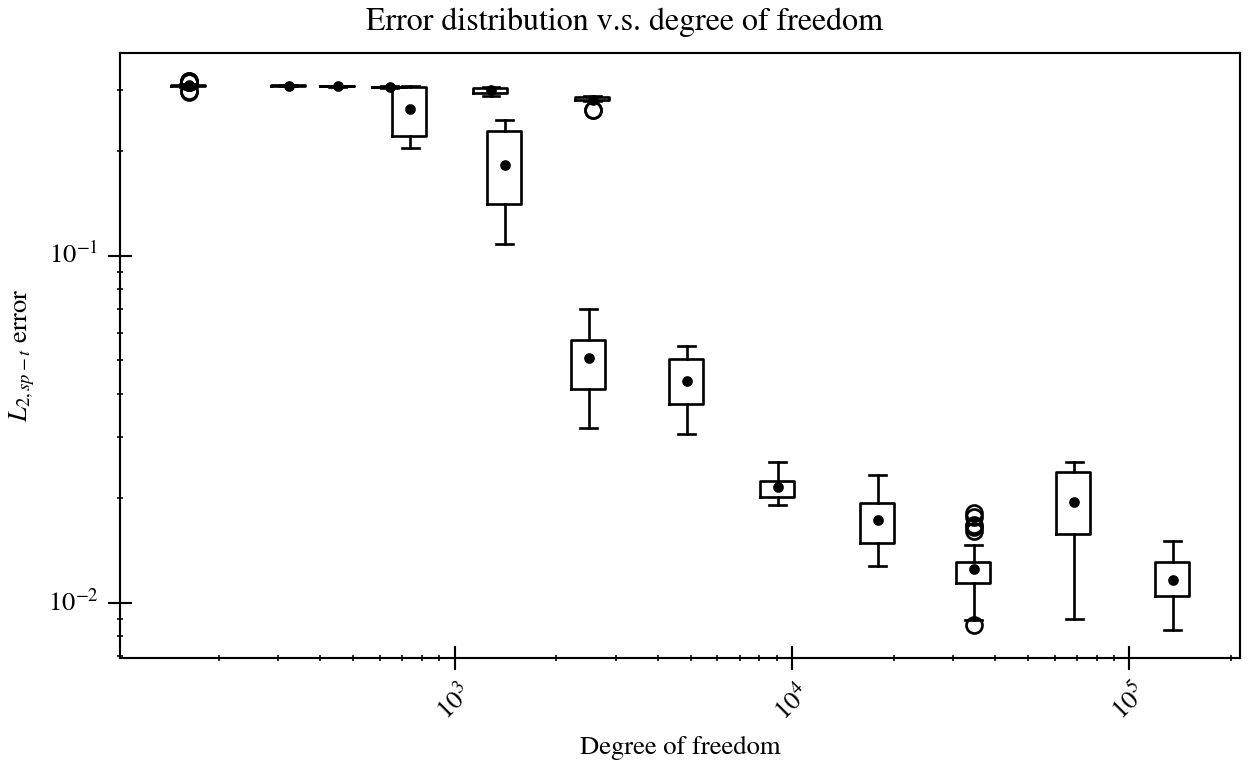
\includegraphics[width=0.95\linewidth]{tgv-2d-re100/err-vs-model-complexity/err-dof-boxplot}
    \caption[%
        PINNs, 2D TGV, $Re=100$: $L_{2,sp-t}$ error v.s. degree of freedom%
    ]{%
        PINNs, 2D TGV, $Re=100$: $L_{2,sp-t}$ error v.s. degree of freedom%
    }
    \label{fig:tgv2d-re100-err-vs-dof}
\end{figure}
From the left portion of the figure, it is obvious that the same number of degrees of freedom does not necessarily give the same accuracy, meaning the model complexity in PINNs can not simply be determined by the number of free parameters in a model.
Also, from the right part of the figure, though increasing the degrees of freedom generally improves the errors, the relationship does not seem to follow a simple monotonically decreasing relationship.
Again, this means the model complexity in PINNs and hence the capability to approximate a complicated flow solution can not be simply determined by the number of free parameters.
This observation also supports the finding that increasing $N_l$ and doubling $N_n$ may have the same effect on the error levels, as the two strategies result in very different numbers of free parameters.

Due to the nonlinearity of PINNs, it is reasonable that the number of free parameters can not be used as a single indicator for how complex an MLP model is.
And to our best knowledge, we have not seen approaches to quantitatively estimate the model complexity.
However, lacking a rigorous understanding of how to evaluate the model complexity in PINNs means, when using PINNs for CFD applications, engineers may not be able to estimate how complicated their PINN models should be to achieve a desired performance.
It further makes it difficult for engineers to evaluate workload, required resources, and costs for engineering projects.

Lastly, figure \ref{fig:tgv2d-re100-err-vs-time} shows the $L_{2,sp-t}$ errors with respect to run times of all cases.
\begin{figure}[hbt!]
    \centering%
    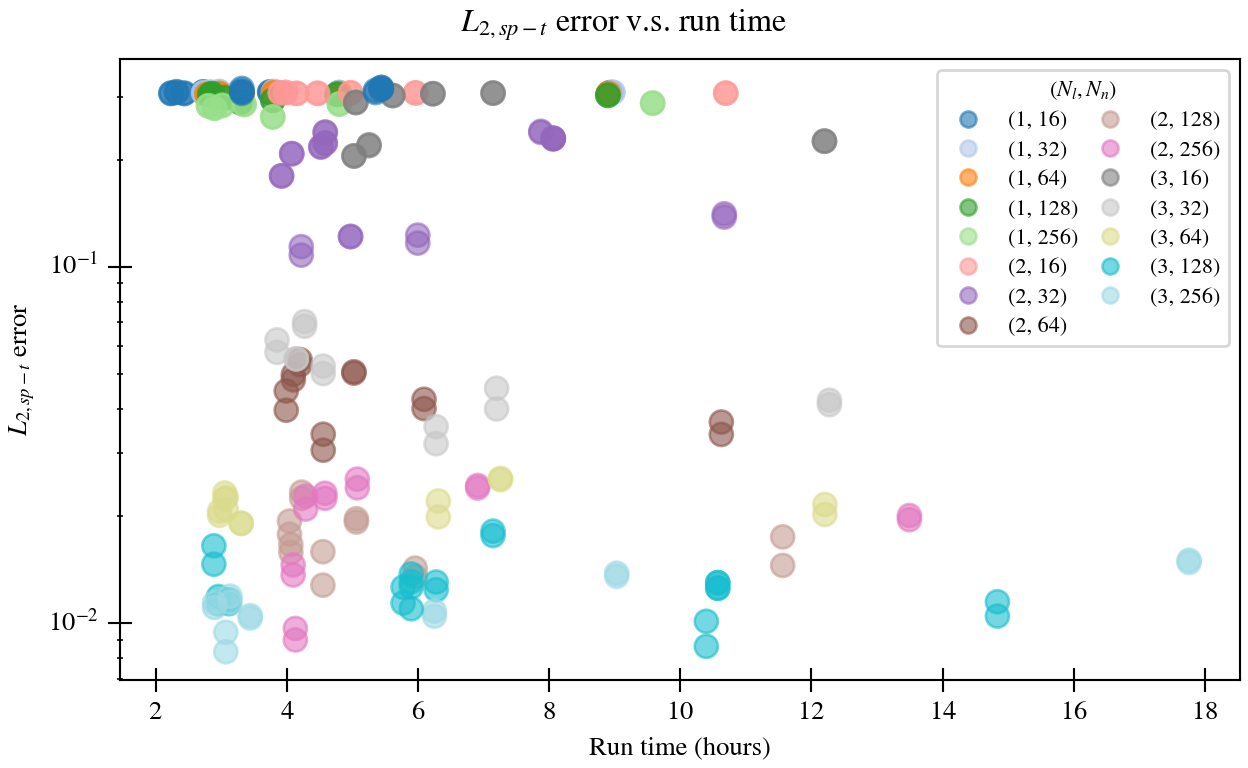
\includegraphics[width=0.95\linewidth]{tgv-2d-re100/err-vs-time/err-time}
    \caption[%
        PINNs, 2D TGV, $Re=100$: $L_{2,sp-t}$ error v.s. run time%
    ]{%
        PINNs, 2D TGV, $Re=100$: $L_{2,sp-t}$ error v.s. run time%
    }
    \label{fig:tgv2d-re100-err-vs-time}
\end{figure}
The colors of dots represent different architectures.
We observed that dots with the same colors are roughly at the same level of errors but are distributed across a wide range of $x$-axis.
It indicates that while $N_{bs}$ has a strong impact on the time costs, it does not have an evident effect on the accuracy.
We did not expect this result because, traditionally in deep learning, using more training data per batch gives a faster convergence and prediction accuracy.
More data per batch means the statistical properties are similar across different batches, and thus the hypersurface does not change significantly from iteration to iteration.
One explanation to the figure \ref{fig:tgv2d-re100-err-vs-time} is that our test cases used too many training points.
The smallest case, $N_{bs}=1024$, might still be big enough for this TGV problem and hence we were not able to see the effect of $N_{bs}$ in the accuracy and convergence rates.
Another explanation is that PINNs are generally insensitive to $N_{bs}$. 
Unfortunately, our test cases are not able to confirm either claim at this point.
If we strictly follow our benchmark results, increasing $N_{bs}$ simply increases the time costs without providing any benefit.
% vim:ft=tex


        \subsection{Training Strategy Investigation}
        \label{sec:pinn-2d-tgv-training-strategy}
        %! TEX root = main.tex
This subsection presents our experiments with several new training strategies, including the annealing loss aggregation, cyclical learning rate, stochastic weight averaging, and the nonlinear conjugate-gradient method.

\subsubsection{Annealing Loss Aggregation}

We applied annealing loss aggregation described in section \ref{sec:loss-annealing} to the cases of $(N_l, N_n, N_{bs}) = (1, 16, 8192)$, $(2, 32, 8192)$, and $(3, 128, 8192)$.
The $\lambda$ parameter in the annealing algorithm is $0.1$ for all cases.
In all the comparisons, we refer to the original loss handling (i.e., equation \eqref{eq:total-residual}) as {\it even-weight aggregation} in the text and {\it naive sum} in the figures to save space.

\begin{figure}[hbt!]
    \centering%
    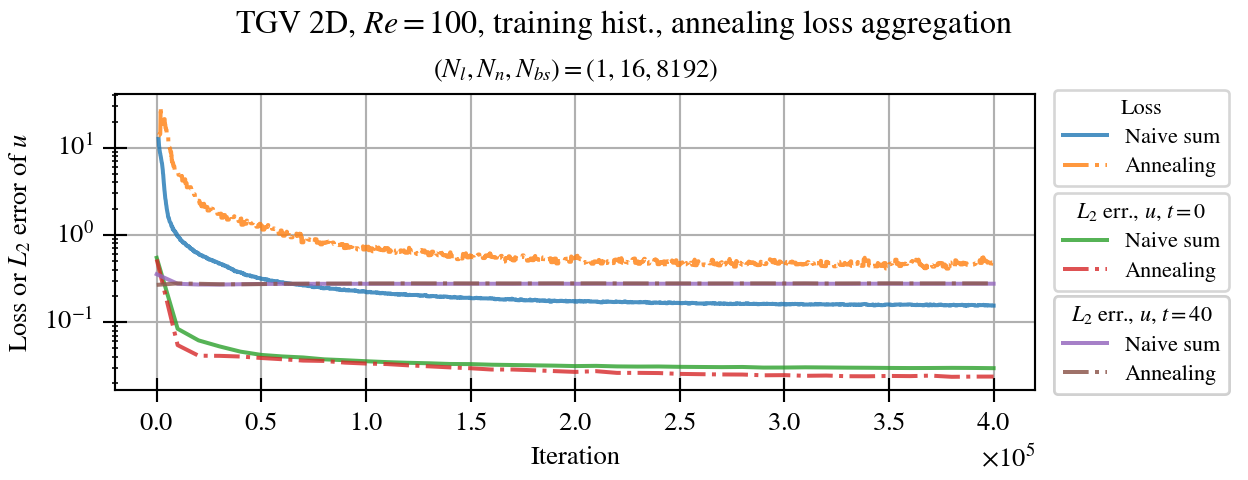
\includegraphics[width=0.9\linewidth]{tgv-2d-re100/annealing-tests/nl1-nn16-npts8192-steps}%
    \caption[%
        Annealing loss aggregation: loss and $L_2$ errors of $u$ v.s. iteration ($(N_l, N_n, N_{bs})=(1, 16, 8192)$)%
    ]{%
        Annealing loss aggregation: loss and $L_2$ errors of $u$ v.s. iteration ($(N_l, N_n, N_{bs})=(1, 16, 8192)$)%
    }\label{fig:annealing-tests-nl1-nn16-npts8192-steps}%
\end{figure}

\begin{figure}[hbt!]
    \centering%
    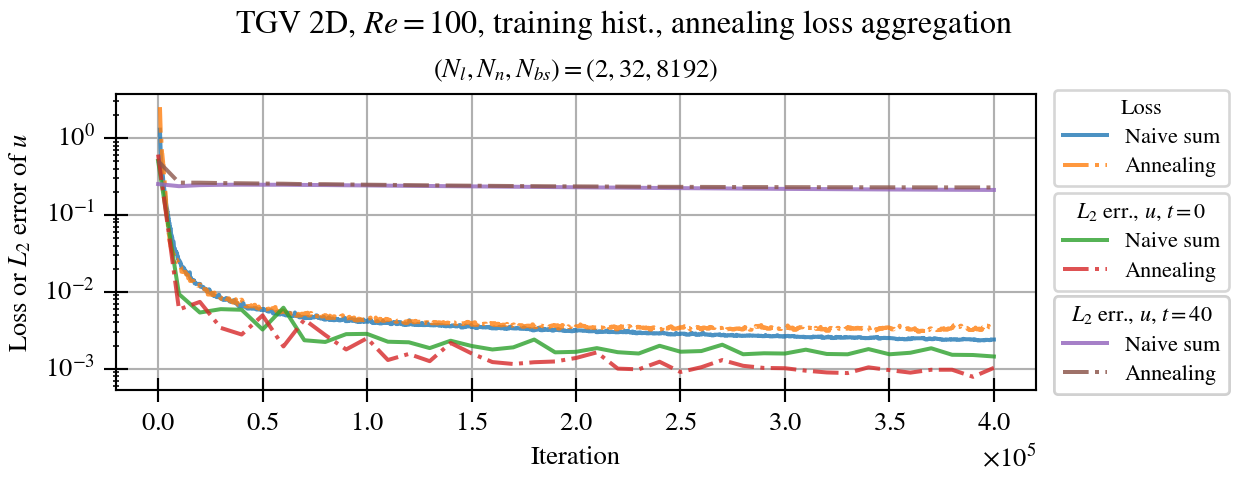
\includegraphics[width=0.9\linewidth]{tgv-2d-re100/annealing-tests/nl2-nn32-npts8192-steps}%
    \caption[%
        Annealing loss aggregation: loss and $L_2$ errors of $u$ v.s. iteration ($(N_l, N_n, N_{bs})=(2, 32, 8192)$)%
    ]{%
        Annealing loss aggregation: loss and $L_2$ errors of $u$ v.s. iteration ($(N_l, N_n, N_{bs})=(2, 32, 8192)$)%
    }\label{fig:annealing-tests-nl2-nn32-npts8192-steps}%
\end{figure}

\begin{figure}[hbt!]
    \centering%
    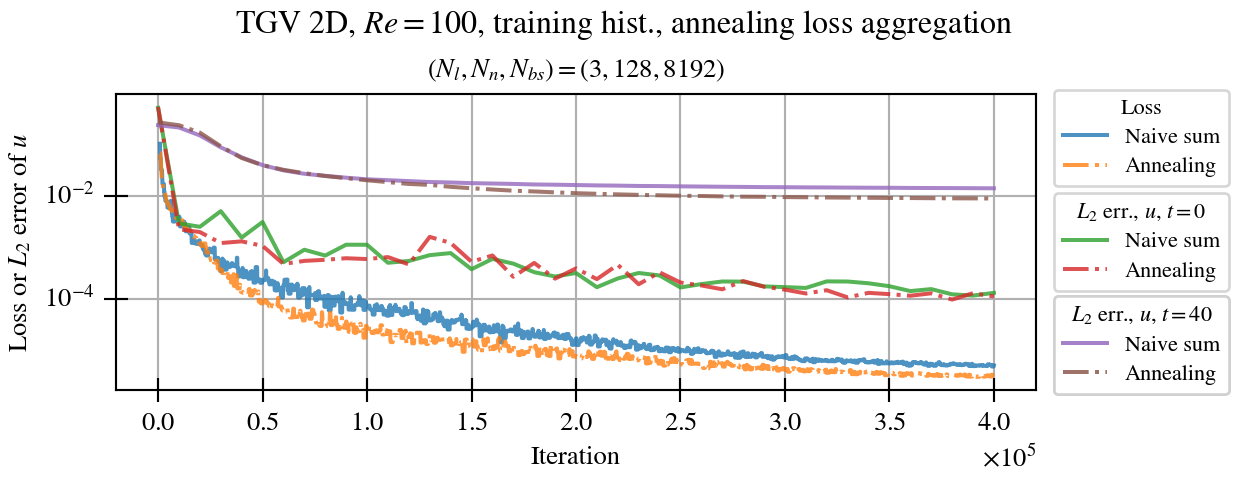
\includegraphics[width=0.9\linewidth]{tgv-2d-re100/annealing-tests/nl3-nn128-npts8192-steps}%
    \caption[%
        Annealing loss aggregation: loss and $L_2$ errors of $u$ v.s. iteration ($(N_l, N_n, N_{bs})=(3, 128, 8192)$)%
    ]{%
        Annealing loss aggregation: loss and $L_2$ errors of $u$ v.s. iteration ($(N_l, N_n, N_{bs})=(3, 128, 8192)$)%
    }\label{fig:annealing-tests-nl3-nn128-npts8192-steps}%
\end{figure}

Figures \ref{fig:annealing-tests-nl1-nn16-npts8192-steps}, \ref{fig:annealing-tests-nl2-nn32-npts8192-steps}, and \ref{fig:annealing-tests-nl3-nn128-npts8192-steps} show the convergence histories of the aggregated losses and errors of $u$.
An interesting observation is that, in figure \ref{fig:annealing-tests-nl1-nn16-npts8192-steps}, the evident gap in the losses of the two algorithms are not reflected in the errors of $u$.
The reason may be that the difference in the losses is due to the different weights of loss terms.
Annealing aggregation may assign a large weight to the IC loss and hence shows a higher aggregated loss.
Other than this observation, we did not observe quantitatively significant difference in both loss and errors between the two algorithms.

Figure \ref{fig:annealing-tests-final-sterrs} gives the comparison of the final $L_{2,sp-t}$ for both $u$ and $v$ velocity.
For simpler network architectures, $(1, 16, 8192)$ and $(2, 32, 8192)$, the final spatial-temporal errors are close.
The more complicated model, $(3, 128, 8192)$, shows visually obvious difference.
However, after examining the actual quantities, we consider them similar.
For example, in the $u$ velocity and with the case of $(3, 128, 8192)$, the even-weight aggregation has an error between $1e-2$ to $2e-2$, while the annealing algorithm has an error between $8e-3$ to $9e-3$.
The difference is just about $20\%$ smaller relative to the even-weight aggregation.
And this difference is even smaller in $v$ velocity.

\begin{figure}[hbt!]
    \centering%
    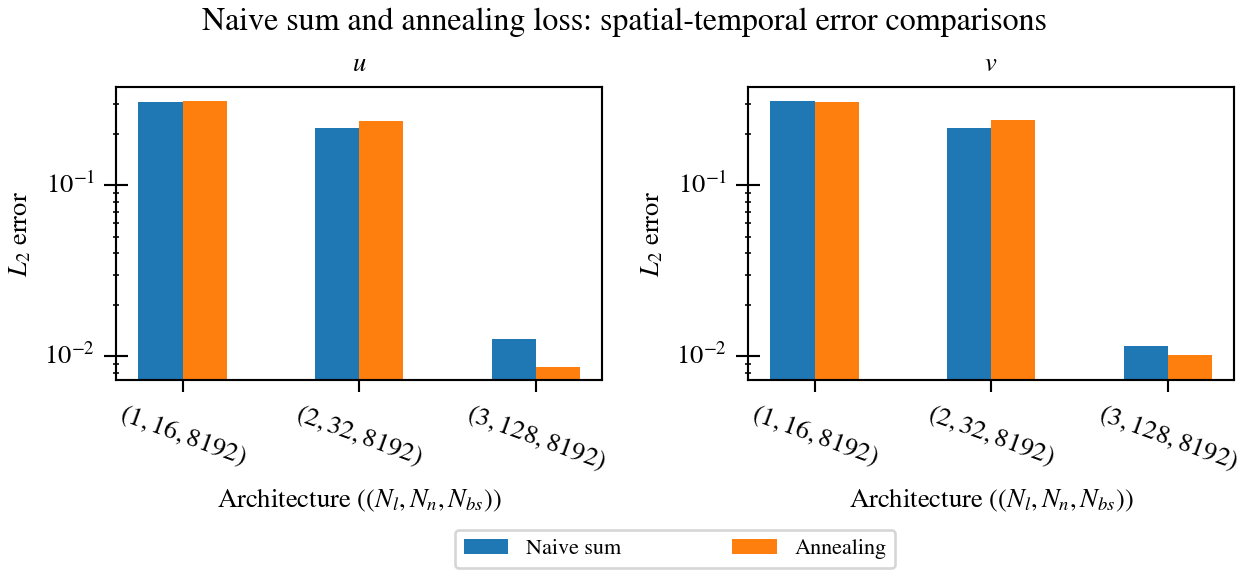
\includegraphics[width=0.9\linewidth]{tgv-2d-re100/annealing-tests/final-spatial-temporal-errors}%
    \caption[%
        Annealing loss aggregation: final spatial-temporal errors%
    ]{%
        Annealing loss aggregation: final spatial-temporal errors%
    }\label{fig:annealing-tests-final-sterrs}%
\end{figure}

We further examined the convergence with respect to the run times.
Annealing loss aggregation is more expensive as it involves evaluating the gradient of each single loss term with respect to model parameters.
As shown in figures \ref{fig:annealing-tests-nl1-nn16-npts8192-walltimes}, \ref{fig:annealing-tests-nl2-nn32-npts8192-walltimes}, and \ref{fig:annealing-tests-nl3-nn128-npts8192-walltimes}, the even-weight aggregation is considered to converge much faster in terms of the run time.
Though annealing aggregation shows a slightly better accuracy at the end of training for $(3, 128, 8192)$, the even-weight aggregation achieves slightly better losses and errors under a given, meaning a better accuracy-cost ratio.
Annealing loss aggregation's computational cost is about the double of the even-weight aggregation. 

\begin{figure}[hbt!]
    \centering%
    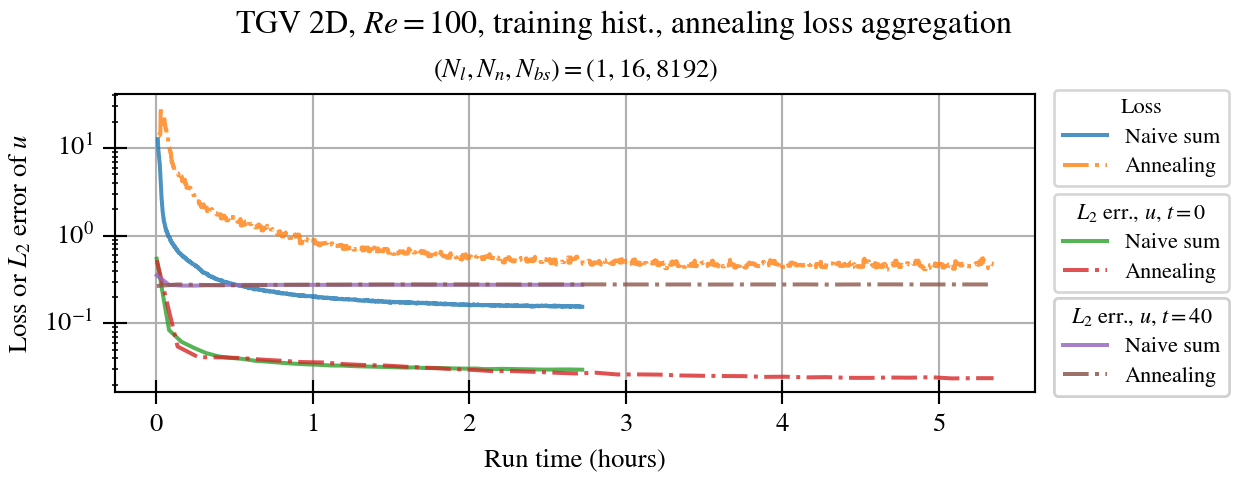
\includegraphics[width=0.9\linewidth]{tgv-2d-re100/annealing-tests/nl1-nn16-npts8192-walltimes}%
    \caption[%
        Annealing loss aggregation: loss and $L_2$ errors of $u$ v.s. wall time ($(N_l, N_n, N_{bs})=(1, 16, 8192)$)%
    ]{%
        Annealing loss aggregation: loss and $L_2$ errors of $u$ v.s. wall time ($(N_l, N_n, N_{bs})=(1, 16, 8192)$)%
    }\label{fig:annealing-tests-nl1-nn16-npts8192-walltimes}%
\end{figure}

\begin{figure}[hbt!]
    \centering%
    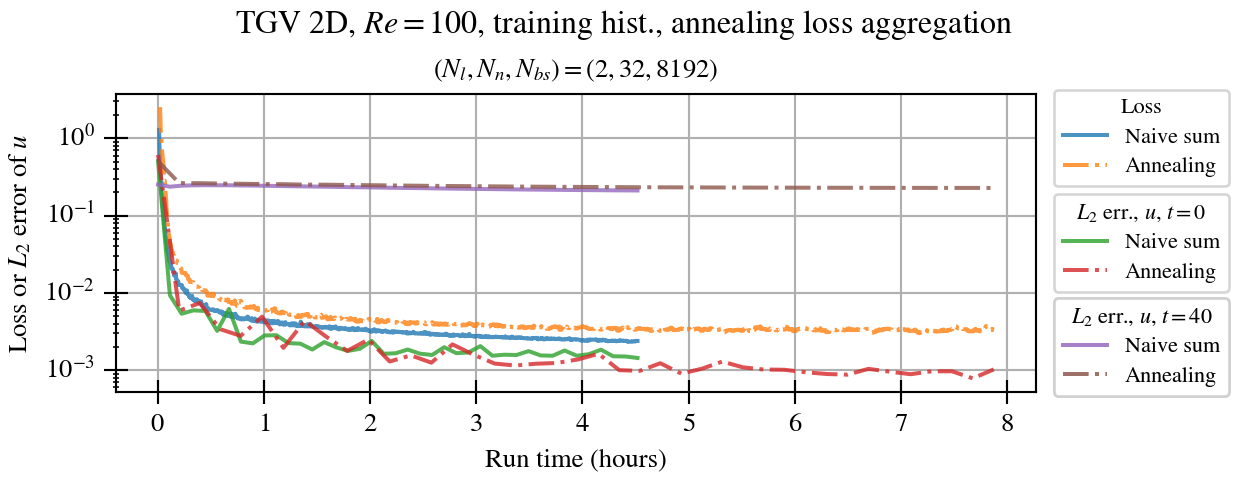
\includegraphics[width=0.9\linewidth]{tgv-2d-re100/annealing-tests/nl2-nn32-npts8192-walltimes}%
    \caption[%
        Annealing loss aggregation: loss and $L_2$ errors of $u$ v.s. wall time ($(N_l, N_n, N_{bs})=(2, 32, 8192)$)%
    ]{%
        Annealing loss aggregation: loss and $L_2$ errors of $u$ v.s. wall time ($(N_l, N_n, N_{bs})=(2, 32, 8192)$)%
    }\label{fig:annealing-tests-nl2-nn32-npts8192-walltimes}%
\end{figure}

\begin{figure}[hbt!]
    \centering%
    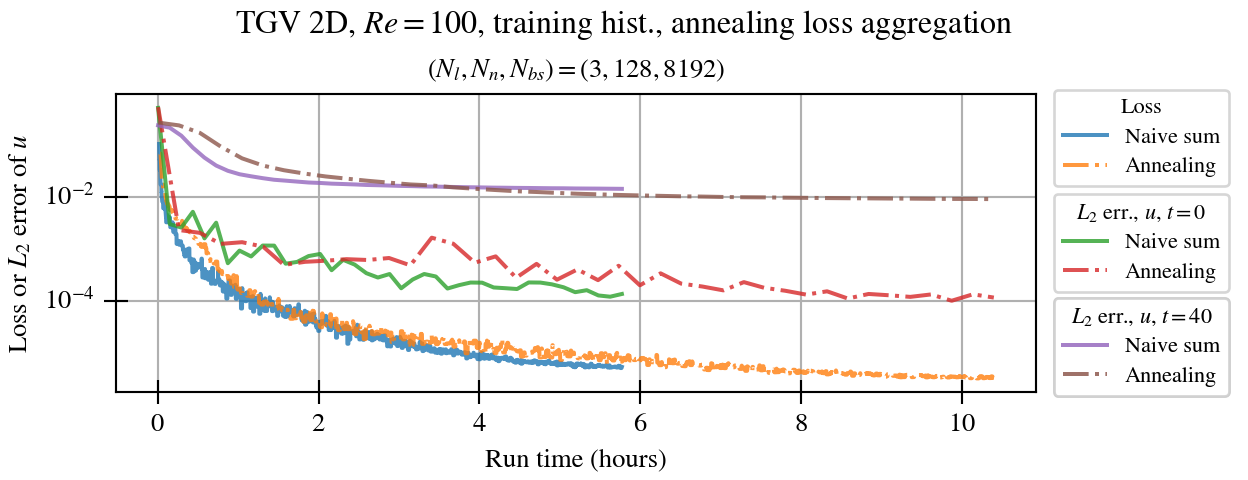
\includegraphics[width=0.9\linewidth]{tgv-2d-re100/annealing-tests/nl3-nn128-npts8192-walltimes}%
    \caption[%
        Annealing loss aggregation: loss and $L_2$ errors of $u$ v.s. wall time ($(N_l, N_n, N_{bs})=(3, 128, 8192)$)%
    ]{%
        Annealing loss aggregation: loss and $L_2$ errors of $u$ v.s. wall time ($(N_l, N_n, N_{bs})=(3, 128, 8192)$)%
    }\label{fig:annealing-tests-nl3-nn128-npts8192-walltimes}%
\end{figure}

\subsubsection{Cyclical Learning Rate and Stochastic Weight Averaging}

The benchmarks in this section cover the cyclical learning rate and stochastic weight averaging (SWA).
The cyclical learning rate (equation \eqref{eq:cyclical-learning-rate}) in this section was configured with $\eta_{low}=1.5e-5$, $\eta_{high}=1.5e-3$, $N_c=5000$, and $\gamma=0.999989$.
Figure \ref{fig:cyclic-swa-tests-lr-hist} shows a comparison of the learning rate from the original exponentially-decaying and the cyclical learning rate.
\begin{figure}[hbt!]
    \centering%
    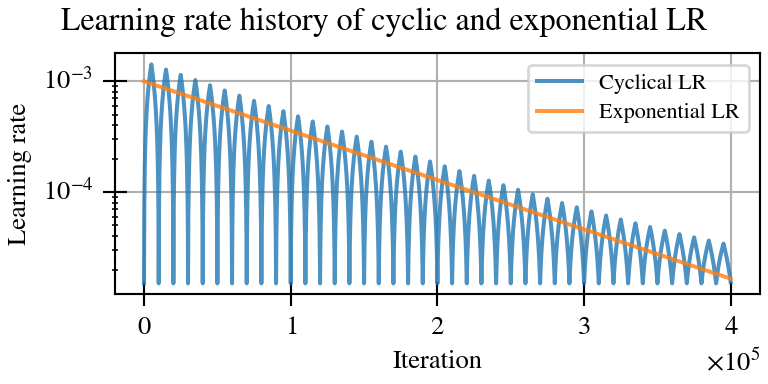
\includegraphics{tgv-2d-re100/cyclic-swa-tests/learning-rate-hist}%
    \caption[%
        Cyclical LR and SWA: learning rate history%
    ]{%
        Cyclical LR and SWA: learning rate history%
    }\label{fig:cyclic-swa-tests-lr-hist}%
\end{figure}
The exponentially-decaying learning rate will be simply denoted as {\it exponential} learning rate in the later discussion and figures.
SWA, on the other, hand, runs in parallel when using cyclical learning rate and does not affect the normal training process.
It is thus able to decouple the performance of SWA from the results of only cyclical learning rate.
In the cases presented here, SWA was configured to collect and average the model parameters from the last 200,000 iterations of the training.
Its results share the same convergence histories with the cases of pure cyclical learning rates.
The only difference between with and without SWA lies in the prediction errors (e.g., errors in $u$) after iteration 200,000.

\begin{figure}[hbt!]
    \centering%
    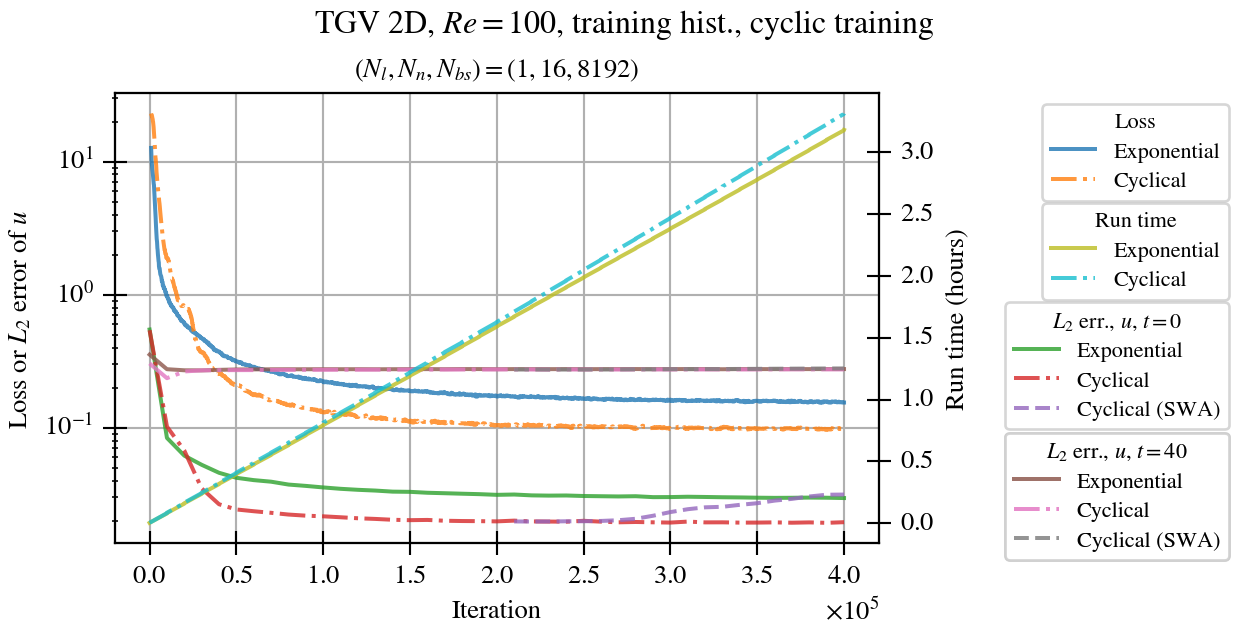
\includegraphics[width=0.9\linewidth]{tgv-2d-re100/cyclic-swa-tests/nl1-nn16-npts8192}%
    \caption[%
        Cyclical LR and SWA: loss and $L_2$ errors of $u$ v.s. iteration ($(N_l, N_n, N_{bs})=(1, 16, 8192)$)%
    ]{%
        Cyclical LR and SWA: loss and $L_2$ errors of $u$ v.s. iteration ($(N_l, N_n, N_{bs})=(1, 16, 8192)$)%
    }\label{fig:cyclic-swa-tests-nl1-nn16-npts8192}%
\end{figure}

\begin{figure}[hbt!]
    \centering%
    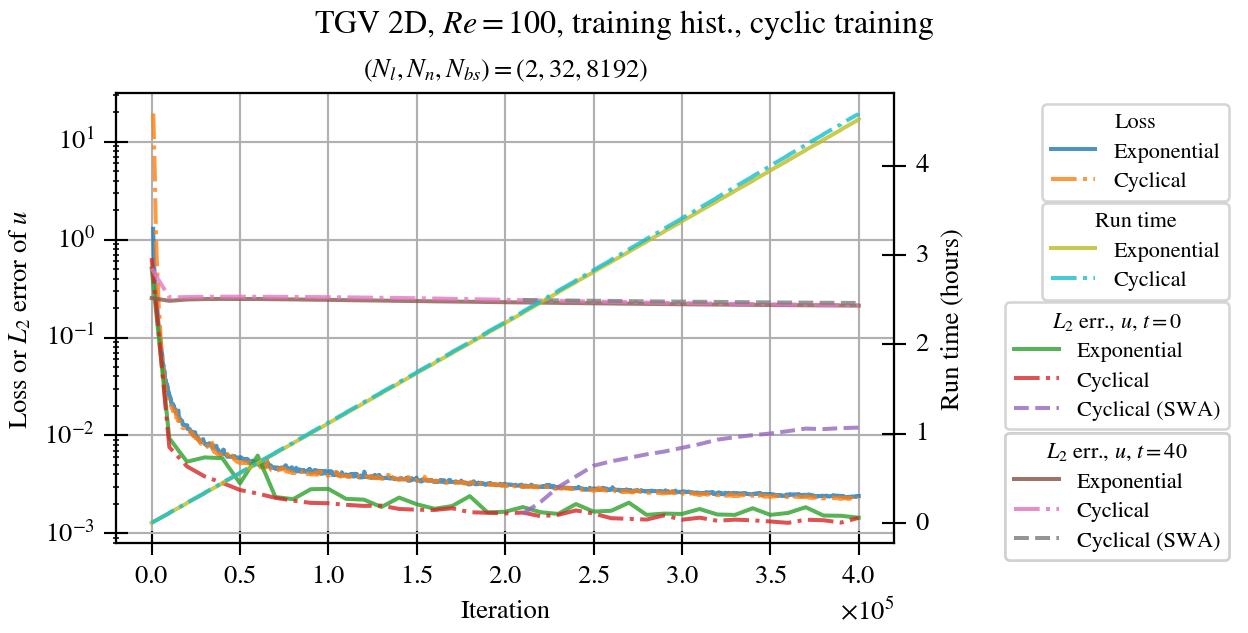
\includegraphics[width=0.9\linewidth]{tgv-2d-re100/cyclic-swa-tests/nl2-nn32-npts8192}%
    \caption[%
        Cyclical LR and SWA: loss and $L_2$ errors of $u$ v.s. iteration ($(N_l, N_n, N_{bs})=(2, 32, 8192)$)%
    ]{%
        Cyclical LR and SWA: loss and $L_2$ errors of $u$ v.s. iteration ($(N_l, N_n, N_{bs})=(2, 32, 8192)$)%
    }\label{fig:cyclic-swa-tests-nl2-nn32-npts8192}%
\end{figure}

\begin{figure}[hbt!]
    \centering%
    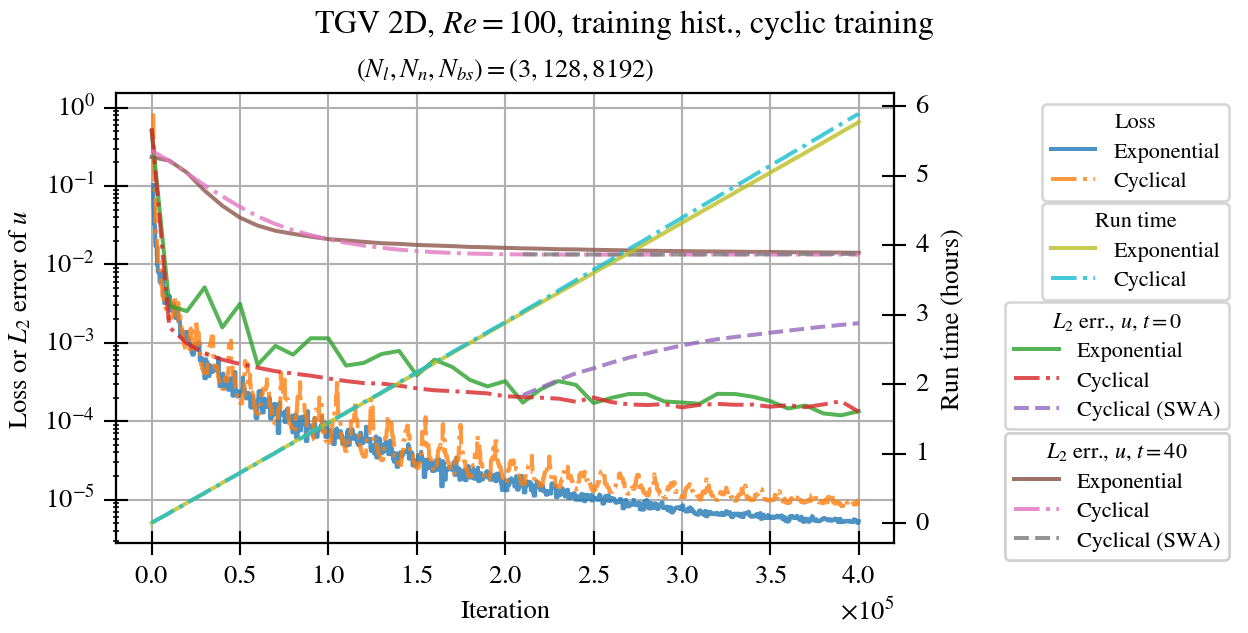
\includegraphics[width=0.9\linewidth]{tgv-2d-re100/cyclic-swa-tests/nl3-nn128-npts8192}%
    \caption[%
        Cyclical LR and SWA: loss and $L_2$ errors of $u$ v.s. iteration ($(N_l, N_n, N_{bs})=(3, 128, 8192)$)%
    ]{%
        Cyclical LR and SWA: loss and $L_2$ errors of $u$ v.s. iteration ($(N_l, N_n, N_{bs})=(3, 128, 8192)$)%
    }\label{fig:cyclic-swa-tests-nl3-nn128-npts8192}%
\end{figure}

In figures \ref{fig:cyclic-swa-tests-nl1-nn16-npts8192}, \ref{fig:cyclic-swa-tests-nl2-nn32-npts8192}, and \ref{fig:cyclic-swa-tests-nl3-nn128-npts8192}, we presented the convergence histories and the time costs.
First, the run times between the two learning rate strategies are similar.
This is expected as cyclical learning rate does not add notable operations to the training.

We next examined the convergence of cyclical and exponentially-decaying learning rates.
The results show that obvious difference only exists in the simplest model, $(1, 16, 8192)$.
However, this difference may be obvious only because the narrower $y$-axis scale in figure \ref{fig:cyclic-swa-tests-nl1-nn16-npts8192}.
If we plot all three figures using the same scale, the difference in $(1, 16, 8192)$ may not be noticeable.
The quantitative difference also supports this claim.
For example, the final loss of exponential learning rate is about $2e-1$, and that of cyclical learning rate is around $1e-1$.
We do not consider this difference significant.

Also, slight oscillation and evident oscillation can be seen in $(2, 32, 8192)$ and $(3, 128, 8192)$, respectively. 
The oscillations may represent how cyclical learning rate helps in escaping local minimums and saddle points. 
The reason that $(1, 16, 8192)$ does not show oscillation may be attributed to the simple hypersurface of $r(\Theta)$.
This architecture may be too simple and may not exhibit complex topography on the hypersurface.

The results in the errors of $u$ show that SWA does not help achieve better predictions at all.
It even hurts the prediction accuracy for $t=0$.
As for $t=40$, for reasons unknown to us at this point, there is no difference.
However, as there is no theory nor guidelines to determine how many iterations should be involved in SWA, the results may be different if using fewer iterations.
Although in this work we did not investigate more on SWA, it could be a potential research question for future studies.

\begin{figure}[hbt!]
    \centering%
    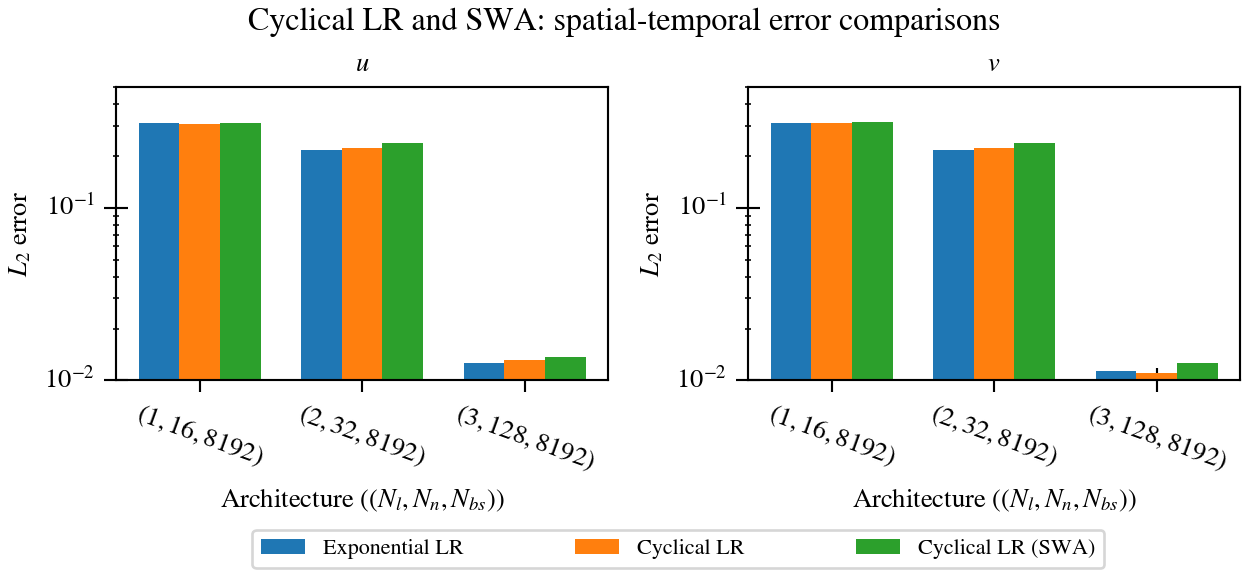
\includegraphics[width=0.9\linewidth]{tgv-2d-re100/cyclic-swa-tests/final-spatial-temporal-errors}%
    \caption[%
        Cyclic LR and SWA: final spatial-temporal errors%
    ]{%
        Cyclic LR and SWA: final spatial-temporal errors%
    }\label{fig:cyclic-swa-tests-final-sterrs}%
\end{figure}

Figure \ref{fig:cyclic-swa-tests-final-sterrs} shows the graphical comparison of the overall spatial-temporal error, $L_{2,sp-t}$.
The results are similar.
Even though SWA gives worse predictions at $t=0$, the integrated error over $t=0$ to $t=100$ does not show significant difference.

\subsubsection{Nonlinear Conjugate-Gradient Optimizer}

The last attempt to adopt new training strategy was the application of nonlinear conjugate-gradient.
The major difficulty of applying CG lies in how to handle batch training.
CG relies on the previous search direction to determine the current search direction, and the former is based on the hypersurface in the last iteration.
In batch training, the hypersurface more or less changes from iteration to iteration due to using different training points.
It is unclear how legit the previous search direction is to be used in the current iteration.

Moreover, in each iteration, the line search algorithm search for a new location along the search direction according to the Wolfe conditions or their derived conditions.
A point meets the Wolfe conditions in the previous iteration does not necessarily meet the same conditions in the current iteration.
This may cause convergence issues in CG as the convergence of CG relies on properly determining the location on each search direction.

Nevertheless, given the efficiencies of CG in non-batched training, we would like to experiment the possibility of using it.
In our current attempt, we used CG to optimize the loss $r(\Theta)$ for a certain batch to a given tolerance before moving on to the next batch.
Also, CG may not have capability to escape from poor local minimums, so our attempts first used Adam for optimization up to 200,000 iterations to identify a region with proper minimum, and then CG was used for an extra 200 iterations.
In other words, pure Adam cases ran 400,000 iterations, while the CG cases ran 200,000 Adam iterations and then 200 iterations with CG.
The case tested are $(1, 16, 8192)$, $(2, 32, 8192)$, and $(3, 128, 8192)$.
CG trained each batch until the change in the loss is smaller than $1e-6$.

\begin{figure}[hbt!]
    \centering%
    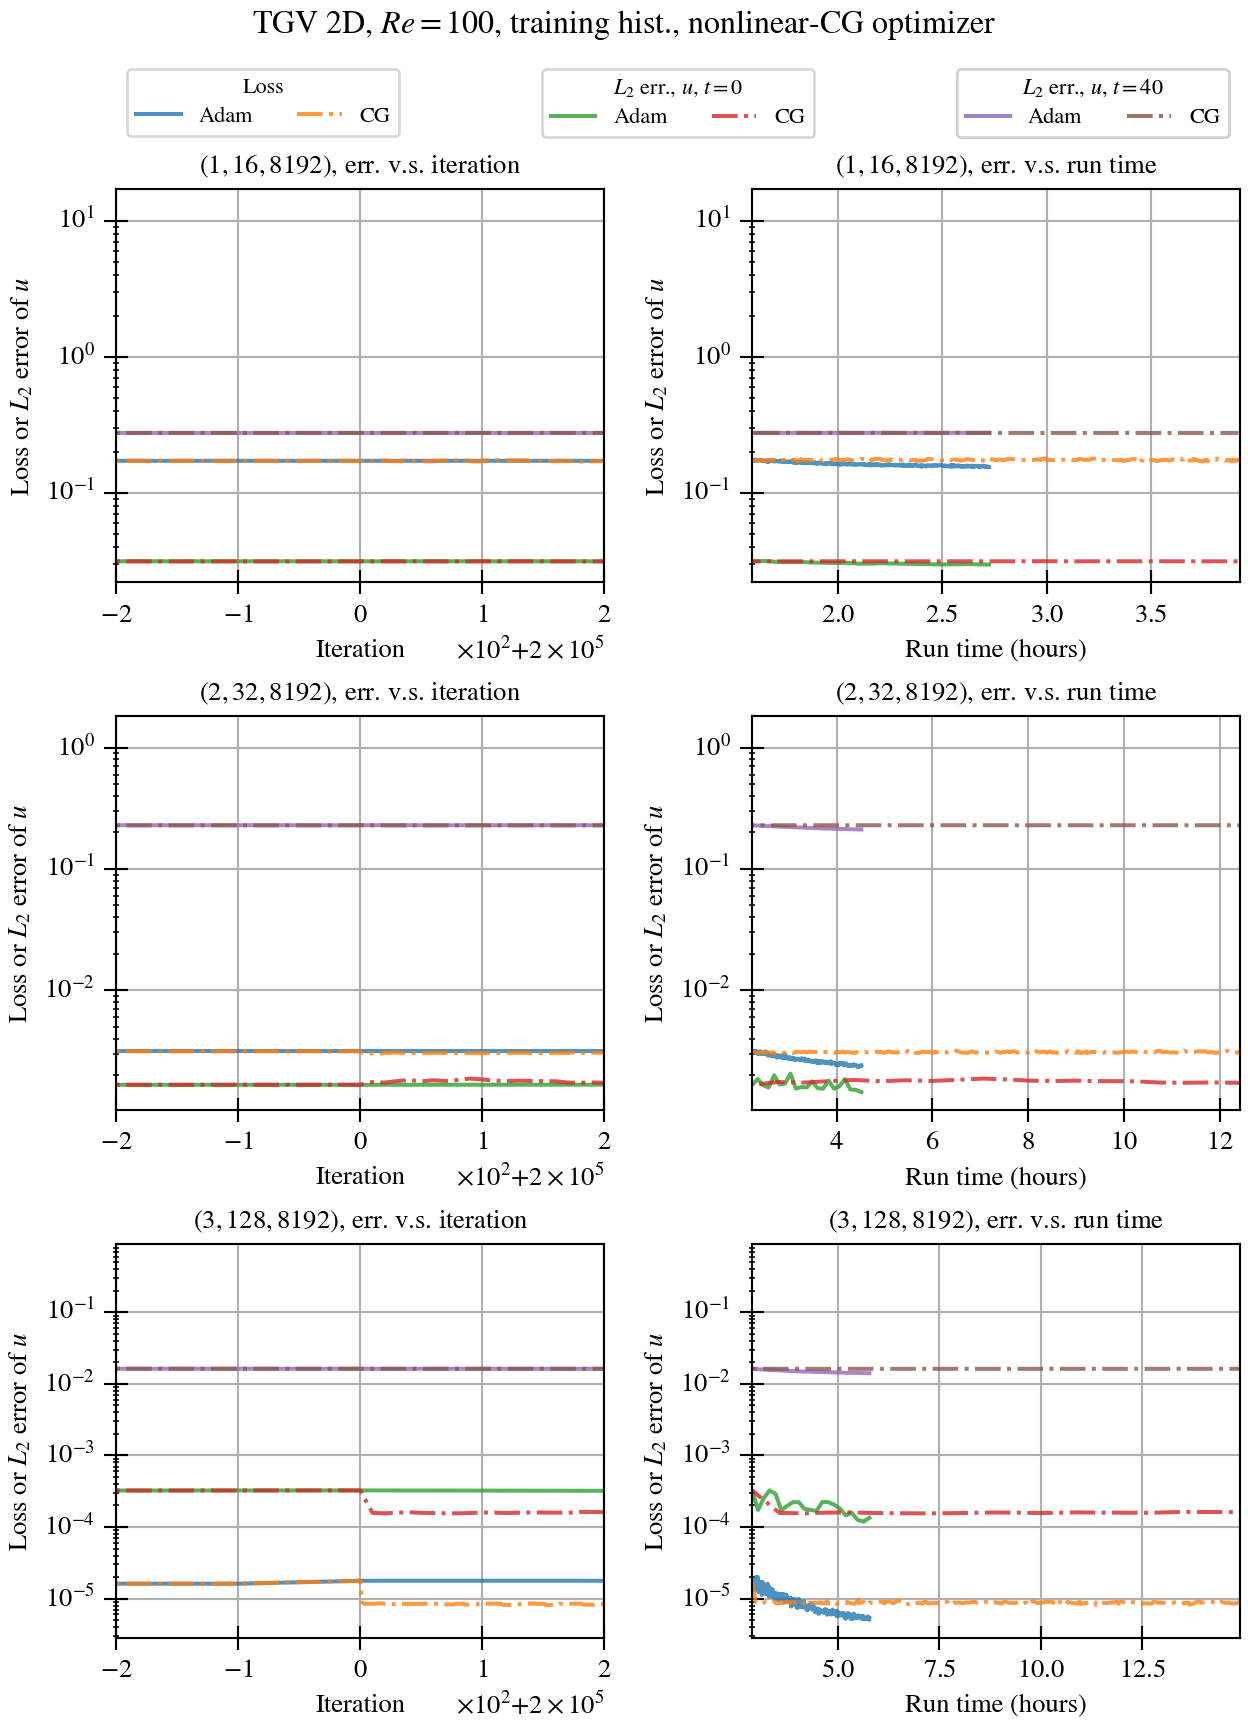
\includegraphics[width=\linewidth]{tgv-2d-re100/ncg-tests/training-hist}%
    \caption[%
        Nonlinear-CG: training history%
    ]{%
        Nonlinear-CG: training history%
    }\label{fig:ncg-tests-train-hist}%
\end{figure}

Figure \ref{fig:ncg-tests-train-hist} shows the comparison of convergence histories between Adam-only cases and CG cases.
On the left we have the losses and errors versus iterations.
The range of iterations shown in the $x$-axis is 199,800th to 200,200th iteration.
We can see for simple architectures, CG does not help reduce the losses.
Based on the observations and discussions in the previous sections, cases with simple architectures converge very early.
It is hence reason for CG not able to improve the losses in simple architectures because they may have already converged.
However, $(3, 128, 8192)$ does show a sudden drop in the loss and error at $t=0$.
After the sudden drop, further training with new batches does not further improve the loss and errors.

On the right of the same figure, we have losses and errors versus run time.
The range of the run time starts from the time for 200,000 iterations until the end of training.
In other words, sub-figures on the right show the 200,000th to 400,000th training iterations for Adam-only cases and 200,000th to 200,200th training iterations for CG cases.
As we use CG on each batch until a certain tolerance, one training iteration with CG consists of hundreds or thousands of sub-iterations inside the CG solver.
Therefore, it is reasonable to see 200 training iterations with CG takes much longer time than 200,000 iterations with Adam.
It is clear from these sub-figures, although CG provides a sudden drop in the losses, it does not further improve the training.
And eventually, Adam reaches even smaller losses than CG does.
More importantly, Adam take much less time.

\begin{figure}[hbt!]
    \centering%
    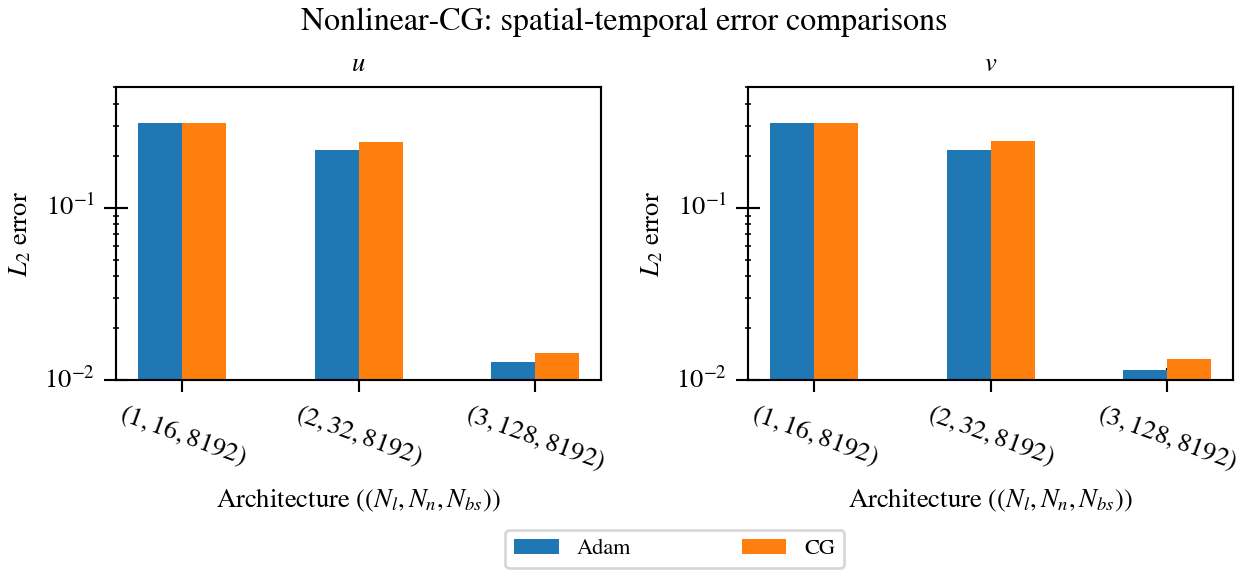
\includegraphics[width=0.9\linewidth]{tgv-2d-re100/ncg-tests/final-spatial-temporal-errors}%
    \caption[%
        Nonlinear-CG: overall spatial-temporal errors%
    ]{%
        Nonlinear-CG: overall spatial-temporal errors%
    }\label{fig:ncg-tests-final-sterrs}%
\end{figure}

Figure \ref{fig:ncg-tests-final-sterrs} shows the final spatial-temporal errors of $u$ and $v$ velocity.
CG does not provide more accurate results.

As mentioned, the major problem with CG is the combined use with batch training and the capability to escape from saddle points and poor minimums.
Carefully tuned line search parameters and algorithm may help achieve the escaping.
However, how to deal with batched training is still a question.
If the issues is caused by the change in hypersurface, then using more training points per batch may help stabilize the hypersurface from iteration to iteration.
And hence each CG iteration is itself a training iteration, i.e., each batch of points is used in one CG iteration.
This may be a potential direction for future investigation on this topic.
% vim:ft=tex

    \section{Steady 2D Cylinder Flow: $Re=40$}
    \label{sec:pinn-2d-cylinder-re40}

        \subsection{Problem Description and Configurations}
        \label{sec:pinn-2d-cylinder-re40-conf}
        %! TEX root = main.tex
The second part of our benchmarking with PINNs focuses on the ability to simulate nonlinear dynamical systems of flow problems.
Our benchmark target is the 2D cylinder flow at $Re=200$, which exhibits vortex shedding.
However, before we conduct the $Re=200$ cylinder flow test, we would like to test a steady cylinder flow problem with our unsteady PINN implementation for solver validation.
The selected case is $Re=40$ cylinder flow, which reaches a steady state eventually.
The results were validated with experimental data and verified against PetIBM results.

The computational domain of the $Re=40$ cylinder flow is $[-10$, $30]$ $\times$ $[-10$, $10]$, and the simulation time range is $t=0$ to $t=20$.
A cylinder with a radius of $0.5$ sits at the coordinate $(0$, $0)$.
Nondimensional density is $1$, and kinematic viscosity is $0.025$, so the Reynolds number is $40$.
The IC is $u=1$ and $v=0$.
The BCs are $u=1$ and $v=0$ on $x=-10$, $y=-10$, and $y=10$.
The BC at the outlet $x=30$ is a 1D convective condition:
\begin{equation}\label{eq:convec-bc}
    \left\{
    \begin{aligned}
        &\pdiff{u}{t} + c\pdiff{u}{\vec{n}} = 0 \\
        &\pdiff{v}{t} + c\pdiff{v}{\vec{n}} = 0 \\
    \end{aligned}
    \right.
\end{equation}
where $\vec{n}$ is the normal vector of the boundary pointing outward from the domain, and $c$ is the convection speed.
In this work, we used $c=1$.

The network used is $(N_l$, $N_n)$ $=$ $(6$, $512)$.
Two PINN implementations were used: a steady solver and an unsteady one.
Two different $N_{bs}$ were used as well to confirm the effect of batch sizes we observed in the previous section: $N_{bs}=\num{6400}$ and $N_{bs}=\num{25600}$.
And we tested two different cyclical learning rate configurations:
\begin{enumerate}[nolistsep]
    \item Large cycle: $(\eta_{low}, \eta_{high}, N_c, \gamma)=(1\times 10^{-6},\ 1\times 10^{-2},\ 5000,\ 0.99998)$
    \item Small cycle: $(\eta_{low}, \eta_{high}, N_c, \gamma)=(1\times 10^{-6},\ 1\times 10^{-3},\ 2000,\ 0.999972)$
\end{enumerate}
Figure \ref{fig:cylinder-2d-re40-lr-hist} shows the comparison of the two schedules.
\begin{figure}[hbt!]
    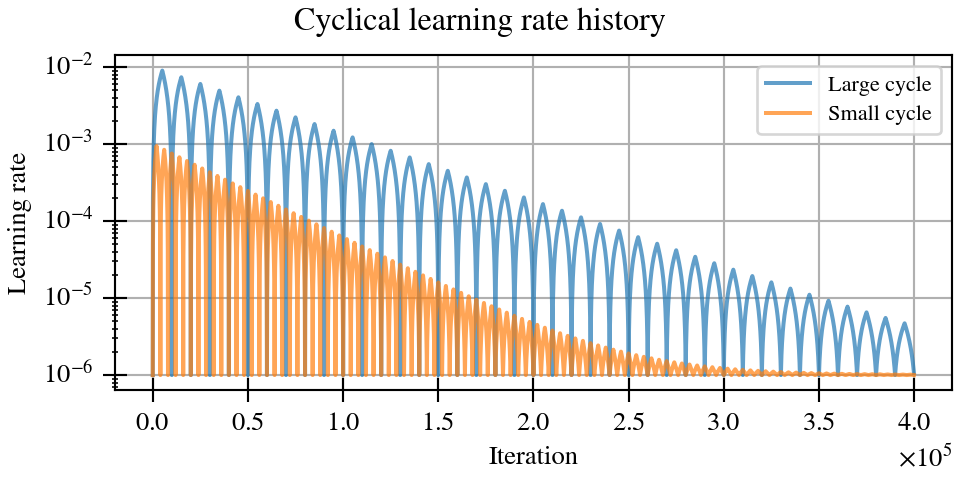
\includegraphics[width=0.9\linewidth]{cylinder-2d-re40/learning-rate-hist}
    \caption[%
        PINNs, 2D Cylinder, $Re=40$: cyclical learning rate configurations%
    ]{%
        PINNs, 2D Cylinder, $Re=40$: cyclical learning rate configurations%
    }%
    \label{fig:cylinder-2d-re40-lr-hist}
\end{figure}
A total of 6 cases were run in this benchmark.
(The small cyclical schedule was not applied to $N_{bs}=\num{25600}$.)

For unsteady cases with $N_{bs}=\num{6400}$, the PINN solver sampled $\num{6400}\times \num{10000}$ points from the computational spatial-temporal domain for PDE losses, meaning each batch was repeated every $\num{10000}$ iterations.
Except for the cylinder surface, $640\times \num{10000}$ points were sampled on each boundary and $t\in[0$, $20]$.
On the cylinder surface, $256\times \num{10000}$ points were sampled and also with $t\in[0$, $20]$.
To evaluate IC losses, $\num{6400}\times \num{10000}$ points were sampled from the spatial domain with their temporal coordinates being constrained to $t=0$.
The steady cases with $N_{bs}=\num{6400}$ follows a similar setting, except the PDE evaluation points were sampled only from spatial domain, as there was no temporal coordinates.
And steady cases did not need to evaluate IC losses.

For cases with $N_{bs}=\num{25600}$, the PDE evaluation points follow the same logic described above.
We used $\num{2560}\times \num{10000}$ points on the boundaries of $y=\pm 10$ and $\num{1280}\times \num{10000}$ points on the boundaries of $x=-10$ and $x=30$.
The cylinder surface had $512\times \num{10000}$ points.

Each case ran for \num{400000} iterations during optimization with the Adam optimizer.
The hardware used was 1 NVIDIA A100 GPU for all cases.

A PetIBM simulation was done as a baseline.
The simulation ran with an NVIDIA K40 GPU with 6 cores of Intel i7-5930K.
Note that the K40 GPU is 5 generations behind the A100 GPU in terms of the technology specification.
The PetIBM simulation resolved the flow on a $562 \times 447$ stretched Cartesian grid with the same computational spatial-temporal domain.
PetIBM used double-precision floats, while PINNs used single precision floats.
The tolerance for all linear solvers in PetIBM was $\num{1e-14}$.
% vim:ft=tex


        \subsection{Results}
        \label{sec:pinn-2d-cylinder-re40-results}
        %! TEX root = main.tex

For steady cases, the PINN solver took about 25 hours to finish for $N_{bs}=25,600$ and 13.5 hours for $N_{bs}=6,400$.
The steady PINN solver, on the other hand, took about 26 hours and 14.5 hours for $N_{bs}=25,600$ and $6,400$, respectively.
The baseline PetIBM simulation was finished within 2 minutes.

Figure \ref{fig:cylinder-2d-re40-loss-hist-steady} shows the convergence history of the aggregated losses for the steady cases, and figure \ref{fig:cylinder-2d-re40-loss-hist-unsteady} shows those for the unsteady cases.
Each figure includes sub-figures for losses against iterations and run times.
\begin{figure}[hbt!]
    \includegraphics[width=0.9\linewidth]{cylinder-2d-re40/loss-hist-steady}
    \caption[
        PINNs, 2D Cylinder, $Re=40$: training history of steady solvers%
    ]{%
        PINNs, 2D Cylinder, $Re=40$: training history of steady solvers%
    }%
    \label{fig:cylinder-2d-re40-loss-hist-steady}
\end{figure}
\begin{figure}[hbt!]
    \includegraphics[width=0.9\linewidth]{cylinder-2d-re40/loss-hist-unsteady}
    \caption[
        PINNs, 2D Cylinder, $Re=40$: training history of unsteady solvers%
    ]{%
        PINNs, 2D Cylinder, $Re=40$: training history of unsteady solvers%
    }%
    \label{fig:cylinder-2d-re40-loss-hist-unsteady}
\end{figure}
An interesting observation from figure \ref{fig:cylinder-2d-re40-loss-hist-steady} is the plateaus at the beginning of the training.
Though without a proof, we suspect this trend reflects the escaping from saddle points.
The large cyclical scheduling took more time to escape because it had fewer cycles under given iterations.
Regardless of the difference at the beginning, all cases reaches the same level of losses eventually.
And for the large cyclical scheduling, both $N_{bs}=6,400$ and $N_{bs}=25,600$ show similar convergence history in terms of iterations.
This observation again proves our suspicion in the previous section that $N_{bs}$ does not have significant influence on the losses and errors..

Figure \ref{fig:cylinder-2d-re40-loss-hist-unsteady} also shows plateaus at the beginning, though not as obvious as those for the steady cases.
The convergence histories for the unsteady cases are also bumpier.
We also suspect that it is caused by escaping from saddle points and poor local minimums.
The hypersurface of unsteady solver might be more complicated than the steady one, hence causing more oscillating convergence.
Nevertheless, all unsteady cases converged to a similar loss level.

Figure \ref{fig:cylinder-2d-re40-contours} shows visual comparisons of the steady-state flow fields.
\begin{figure}[hbt!]
    \includegraphics[width=\linewidth]{cylinder-2d-re40/contour-comparison}
    \caption[
        PINNs, 2D Cylinder, $Re=40$: flow fields at steady state%
    ]{%
        PINNs, 2D Cylinder, $Re=40$: flow fields at steady state%
        For the unsteady PINN case, the solution was extracted from $t=20$.
        The fields shown, from the top to bottom, are $u$, $v$, $p$, and vorticity $\omega_z$.
    }%
    \label{fig:cylinder-2d-re40-contours}
\end{figure}
The results of steady PINN solver were obtained from the case of $N_{bs}=25,600$ with the large cyclical scheduling, and that of the unsteady solver was also obtained from the same $N_{bs}$ and scheduling.
All three cases visually agree with each other, except for the vorticity.
Note that vorticity is a product from post-processing for all three solvers.
PetIBM relies on central difference to calculate the vorticity.
And PINNs use automatic differentiation to obtain it.

Figure \ref{fig:cylinder-2d-re40-drag-lift-time} gives the drag and lift coefficients ($C_D$ and $C_L$).
We only plotted the results from the unsteady solver because the steady solvers do not have the time variable. 
\begin{figure}[hbt!]
    \includegraphics[width=\linewidth]{cylinder-2d-re40/drag-lift-coeffs.png}
    \caption[
        PINNs, 2D Cylinder, $Re=40$: drag and lift coefficients%
    ]{%
        PINNs, 2D Cylinder, $Re=40$: drag and lift coefficients%
    }%
    \label{fig:cylinder-2d-re40-drag-lift-time}
\end{figure}
Table \ref{table:cylinder-2d-re40-comparison-cd} compares the values of $C_D$ against the experimental data and simulation data from other groups.
\begin{table}[hbt!]
    \singlespacing
    \begin{threeparttable}[b]
        \begin{tabular}{lccc}
            \toprule
            & $C_D$ & $C_{D_p}$ & $C_{D_f}$ \\
            \midrule
            $(6, 512, 6400)$, steady & 1.62 & 1.07 & 0.55 \\
            $(6, 512, 6400)$, unsteady & 1.63 & 1.02 & 0.61 \\
            $(6, 512, 6400)$, large cycle, steady & 1.62 & 1.07 & 0.55 \\
            $(6, 512, 6400)$, large cycle, unsteady & 1.53 & 0.96 & 0.57 \\
            $(6, 512, 25600)$, large cycle, steady & 1.62 & 1.06 & 0.55 \\
            $(6, 512, 25600)$, large cycle, unsteady & 1.60 & 1.06 & 0.55 \\
            PetIBM & 1.63 & 1.02 & 0.61 \\
            Rosetti et al., 2012\cite{rosetti_urans_2012}\tnote{1} & 1.74\pm 0.09 & n/a & n/a \\
            Rosetti et al., 2012\cite{rosetti_urans_2012}\tnote{2} & 1.61 & n/a & n/a \\
            Sen et al., 2009\cite{sen_steady_2009}\tnote{2} & 1.51 & n/a & n/a \\
            Park et al., 1988\cite{park_numerical_1998}\tnote{2} & 1.51 & 0.99 & 0.53 \\
            Tritton, 1959\cite{tritton_experiments_1959}\tnote{1} & 1.48--1.65 & n/a & n/a \\
            Grove et al., 1964\cite{grove_experimental_1964}\tnote{1} & n/a & 0.94 & n/a \\
            \bottomrule
        \end{tabular}%
        \begin{tablenotes}
            \footnotesize
            \item [1] Experimental result
            \item [2] Simulation result
        \end{tablenotes}
        \caption[PINNs, 2D Cylinder, $Re=40$: validation of drag coefficients]{%
            Validation of drag coefficients.%
            $C_D$, $C_{D_p}$, and $C_{D_f}$ denote the coefficients of total drag, pressure drag, %
            and friction drag, respectively.%
        }%
        \label{table:cylinder-2d-re40-comparison-cd}
    \end{threeparttable}
\end{table}%

As seen from the table, values from different previous works in the literature show a variability in $C_D$.
Though there is not a correct answer to compare against, at least the $C_D$ from PINNs and PetIBM all fall into the range of others' works.
And the differences seen in figure \ref{fig:cylinder-2d-re40-drag-lift-time} is acceptable given that the $C_D$ shown in the figure are all within the acceptable range.
We consider the results of $C_D$ is validated.

Lastly, we compared the pressure coefficient ($C_p$) on the cylinder surface.
Figure \ref{fig:cylinder-2d-re40-surface-cp-steady} shows the surface $C_p$ of the steady cases, and figure \ref{fig:cylinder-2d-re40-surface-cp-unsteady} shows that of the unsteady cases.
\begin{figure}[hbt!]
    \includegraphics[width=0.9\linewidth]{cylinder-2d-re40/surface-pressure-steady}
    \caption[
        PINNs, 2D Cylinder, $Re=40$: pressure coefficients on cylinder surface for steady solvers%
    ]{
        PINNs, 2D Cylinder, $Re=40$: pressure coefficients on cylinder surface for steady solvers%
        The data from Grove et al., 1964 are experimental, while others are computational.
    }%
    \label{fig:cylinder-2d-re40-surface-cp-steady}
\end{figure}
\begin{figure}[hbt!]
    \includegraphics[width=0.9\linewidth]{cylinder-2d-re40/surface-pressure-unsteady}
    \caption[
        PINNs, 2D Cylinder, $Re=40$: pressure coefficients on cylinder surface for unsteady solvers%
    ]{
        PINNs, 2D Cylinder, $Re=40$: pressure coefficients on cylinder surface for unsteady solvers%
        The data from Grove et al., 1964 are experimental, while others are computational.
    }%
    \label{fig:cylinder-2d-re40-surface-cp-unsteady}
\end{figure}
As there is no correct answer, we consider the results of the surface $C_p$ validated.
All results from PINNs are visually within the range made up by the reference data.
% vim:ft=tex

    \section{Unsteady 2D Cylinder Flow: Vortex Shedding at $Re=200$}
    \label{sec:pinn-2d-cylinder-re200}

        \subsection{Problem Description and Configurations}
        \label{sec:pinn-2d-cylinder-re200-conf}
        %! TEX root = main.tex
With the successful validation for the $Re=40$ cylinder flow, we now would like to test an unsteady cylinder flow at $Re=200$.

The computational spatial domain is $[-8$, $25]$ $\times$ $[-8$, $8]$, and the simulation time range is $t\in[0$, $200]$.
Other problem setups are the same as those in section \ref{sec:pinn-2d-cylinder-re40-conf}, except for the kinematic viscosity.
The non-dimensional kinematic viscosity is $0.005$ to make the Reynolds number $200$.

The network architecture is the same: $(N_l$, $N_n)$ $=$ $(6$, $512)$.
We also used a steady and an unsteady PINN solver on this problem, though $Re=200$ is not expected to have a steady-state solution.
The batch size and the configurations of training points are the same as the case of $N_{bs}=\num{6400}$ in section \ref{sec:pinn-2d-cylinder-re40-conf}.
We only used one cyclical learning rate schedule: $(\eta_{low}$, $\eta_{high}$, $N_c$, $\gamma)$ $=$ $(\num{1e-6}$, $\num{1e-2}$, $5000$, $0.9999915)$.

In addition to the steady and unsteady PINN solvers, a third case was done in this benchmark.
This case is a data-driven PINN simulation.
In this data-driven PINN case, we removed the original IC and train the PINN model against several snapshots from a PetIBM simulation.
The selected snapshots from PetIBM were those at $t=125$, $126$, $\cdots$, $139$, $140$.
These snapshots contain around $3$ full periods of vortex shedding.
In other words, we replaced the IC loss terms in equation \eqref{eq:total-residual} with  
\begin{equation}\label{eq:data-driven-loss}
    \left\{
        \begin{aligned}
            &r_{data,\vec{u}}(\Theta) = \sum\limits_{i=1}^{N_{data}}\lVert G_i^{\vec{u}} - \vec{u}_{data, i}\rVert^2 \\
            &r_{data,p}(\Theta) = \sum\limits_{i=1}^{N_{data}}\left( G_i^{p} - p_{data, i} \right)^2
        \end{aligned}
    \right.
\end{equation}
where subscript $data$ denotes the data from the PetIBM simulation.
The total number of data points from PetIBM is around $\num{17000000}$, and we only used $\num{6400}$ every iteration, meaning each data batch was repeated approximately every $\num{2650}$ iterations.
Except for replacing the IC losses with a data-driven approach, all other loss terms in \eqref{eq:total-residual} remain the same.

Note that for the data-driven case, the loss terms of PDEs and BCs were evaluated only in $t\in[125$, $200]$ because we treated PetIBM's data as if they were ICs.
Also, because PDEs were solved even after $t=140$ (the last snapshot from PetIBM), we expected this trained model to be able to make predictions for $t>140$.

Each case ran for $\num{1000000}$ iterations with the Adam optimizer.
The hardware used was 1 NVIDIA A100 GPU for all cases.

The mentioned PetIBM simulation was done on the same K40 configuration as described in section \ref{sec:pinn-2d-cylinder-re40-conf}.
The solver configuration is the same as well, except that the grid resolution is $1485$ $\times$ $720$.
% vim:ft=tex


        \subsection{Results}
        \label{sec:pinn-2d-cylinder-re200-results}
        %! TEX root = main.tex
The overall run times for the steady, unsteady, and data-driven cases are about 28 hours, 31 hours, and 33.5 hours.
The PetIBM simulation, on the other hand, took around 1.7 hours with a 5-generation-behind GPU.

Figure \ref{fig:cylinder-re200-train-hist} shows the convergence history of all cases.
\begin{figure}[hbt!]
    \includegraphics[width=0.9\linewidth]{cylinder-2d-re200/loss-hist}
    \caption{PINNs, 2D Cylinder, $Re=200$: training history}
    \label{fig:cylinder-re200-train-hist}
\end{figure}
One sub-plot is for losses versus iterations, while the other one is against the run times.
The plateaus we observed in the $Re=40$ cases also exist in the unsteady and data-driven cases here.
The steady case does not show any sign of the plateau.
The data-driven case does not converge to a loss level as small as that of the other two cases.
However, the aggregated loss of the data-driven case has extra data loss terms, so it is unclear at this point if all loss terms have higher values or only the data loss terms are higher. 

\begin{table}[hbt!]
    \singlespacing
    \begin{threeparttable}[b]
        \begin{tabular}{lcc}
            \toprule
            & $C_D$ \\
            \midrule
            PetIBM & 1.38   \\
            Steady PINN & 0.95 \\
            Unsteady PINN & 0.95 \\
            Deng et al., 2007\cite{deng_hydrodynamic_2007}\tnote{1} & 1.25 \\
            Rajani et al., 2009\cite{Rajani2009}\tnote{1} & 1.34 \\
            Gushchin \& Shchennikov, 1974\cite{gushchin_numerical_1974}\tnote{2} & 0.97 \\
            Fornberg, 1980\cite{fornberg_numerical_1980}\tnote{2} & 0.83 \\
            \bottomrule
        \end{tabular}%
        \begin{tablenotes}
            \footnotesize
            \item [1] Unsteady simulations.
            \item [2] Steady simulations.
        \end{tablenotes}
        \caption[
            PINNs, 2D Cylinder, $Re=200$: validation of drag coefficients%
        ]{%
            PINNs, 2D Cylinder, $Re=200$: validation of drag coefficients.%
            The data-driven case is excluded because it does not have an obvious periodic state nor a steady-state solution.%
        }%
        \label{table:cylinder-2d-re200-cd}
    \end{threeparttable}
\end{table}%


\begin{figure}[hbt!]
    \includegraphics[width=0.9\linewidth]{cylinder-2d-re200/drag-lift-coeffs}
    \caption{PINNs, 2D Cylinder, $Re=200$: drag and lift coefficients}
    \label{fig:cylinder-re200-drag-lift}
\end{figure}

Figure \ref{fig:cylinder-re200-drag-lift} shows the drag and lift coefficients versus simulation time.
The coefficients from the steady case is just a horizontal line because there is no time variable in this case.
The unsteady case, to our surprise, does not exhibit oscillation, meaning probably no vortex shedding.
Although, it fits well with the PetIBM result before shedding happens (before around $t=75$), including the wake development stage before $t=25$.
Comparing the coefficients between the steady, unsteady, and PetIBM's values before shedding, we believe the unsteady PINN in this particular case behaves just like a steady solver.
This speculation is further supported by the values in table \ref{table:cylinder-2d-re200-cd}, where we compare $C_D$ to both unsteady and steady numerical simulations from literature.
The $C_D$ obtained from the unsteady PINN is the same as the steady PINN and close to those steady CFD simulation results.

As for the data-driven case, its temporal domain is $t\in[125$, $200]$, so the coefficients' trajectories start from $t=125$.
The result, again unexpected to us, only exhibits shedding in the time range where we provide data with shedding to the PINN ($t\in[125$, $140]$).
This result also shows that data-driven PINNs may be more difficult to train, compared to data-free PINNs and regular data-only model fitting.
Even in the range of provided data, the data-driven case is not able to reach the given maximal $C_L$, and the $C_D$ is obviously off from the given data.
After $t=140$, the trajectories quickly fall back to the no-shedding pattern, though it still deviates from the trajectories of the steady and unsteady PINNs.
Combining the loss magnitude shown in figure \ref{fig:cylinder-re200-train-hist}, the deviation of values may be caused by not enough training.
As figure \ref{fig:cylinder-re200-train-hist} shows data-driven PINN is converged, other optimization techniques or hyperparameter tuning may be required to further reduce the loss.

Nevertheless, we believe not being trained enough only explains why the data-driven case deviates from the given data and the trajectories of the other two cases.
Even with a better optimization and eventually a lower loss, based on the trajectories, we do not believe the shedding will continue after $t=140$.

To examine how the transient flow develops, below we show several snapshots of the flow fields from PetIBM and PINNs:
\begin{enumerate}
    \item Figure \ref{fig:cylinder-re200-contour-steady} shows the flow field obtained from the steady PINN as a reference.
    \item Figures \ref{fig:cylinder-re200-contour-uv-t10} and \ref{fig:cylinder-re200-contour-pwz-t10}: flow at $t=10$. We can see the wake is still developing, and the unsteady PINN visually matches PetIBM. It means the unsteady PINN is indeed an unsteady solver. This time is out of the data-driven PINN's temporal domain.
    \item Figures \ref{fig:cylinder-re200-contour-uv-t50} and \ref{fig:cylinder-re200-contour-pwz-t50}: flow at $t=50$. These figures further confirm that the unsteady PINN matches the PetIBM simulation before shedding.
    \item Figures \ref{fig:cylinder-re200-contour-uv-t140} and \ref{fig:cylinder-re200-contour-pwz-t140}: flow at $t=140$. At this point, the shedding already happened. And $t=140$ is the last snapshot we fed to the data-driven PINN for training. The flow from data-driven PINN shows that it at least is able to qualitatively capture the shedding, which is expected.
    \item Figures \ref{fig:cylinder-re200-contour-uv-t144} and \ref{fig:cylinder-re200-contour-pwz-t144}: flow at $t=144$. Just $4$ unit time from the last snapshot we fed to the data-driven PINN, the data-driven PINN has already stopped generating new vortices. The existing vortex can be seen moving toward the boundary, and the wake is gradually recovering to the steady state wake.
    \item Figures \ref{fig:cylinder-re200-contour-uv-t190} and \ref{fig:cylinder-re200-contour-pwz-t190}: flow at $t=190$. Flow field at this time further confirms that the data-driven PINN's behavior is leaning toward that of the unsteady PINN, which is itself behaving like a steady state solver.
\end{enumerate}

\begin{figure}[hbt!]
    \includegraphics[width=0.9\linewidth]{cylinder-2d-re200/contour-comparison-steady}
    \caption{2D Cylinder, $Re=200$: flow field contours for steady PINN}
    \label{fig:cylinder-re200-contour-steady}
\end{figure}

\begin{figure}[hbt!]
    \includegraphics[width=0.9\linewidth]{cylinder-2d-re200/contour-comparison-uv-t10}
    \caption{2D Cylinder, $Re=200$: flow field comparisons for $u$ and $v$ at $t=10$ (PetIBM, data-driven PINN, and data-free PINN)}
    \label{fig:cylinder-re200-contour-uv-t10}
\end{figure}

\begin{figure}[hbt!]
    \includegraphics[width=0.9\linewidth]{cylinder-2d-re200/contour-comparison-pwz-t10}
    \caption{2D Cylinder, $Re=200$: flow field comparisons for $p$ and $\omega_z$ at $t=10$ (PetIBM, data-driven PINN, and data-free PINN)}
    \label{fig:cylinder-re200-contour-pwz-t10}
\end{figure}

\begin{figure}[hbt!]
    \includegraphics[width=0.9\linewidth]{cylinder-2d-re200/contour-comparison-uv-t50}
    \caption{2D Cylinder, $Re=200$: flow field comparisons for $u$ and $v$ at $t=50$ (PetIBM, data-driven PINN, and data-free PINN)}
    \label{fig:cylinder-re200-contour-uv-t50}
\end{figure}

\begin{figure}[hbt!]
    \includegraphics[width=0.9\linewidth]{cylinder-2d-re200/contour-comparison-pwz-t50}
    \caption{2D Cylinder, $Re=200$: flow field comparisons for $p$ and $\omega_z$ at $t=50$ (PetIBM, data-driven PINN, and data-free PINN)}
    \label{fig:cylinder-re200-contour-pwz-t50}
\end{figure}

\begin{figure}[hbt!]
    \includegraphics[width=0.9\linewidth]{cylinder-2d-re200/contour-comparison-uv-t140}
    \caption{2D Cylinder, $Re=200$: flow field comparisons for $u$ and $v$ at $t=140$ (PetIBM, data-driven PINN, and data-free PINN)}
    \label{fig:cylinder-re200-contour-uv-t140}
\end{figure}

\begin{figure}[hbt!]
    \includegraphics[width=0.9\linewidth]{cylinder-2d-re200/contour-comparison-pwz-t140}
    \caption{2D Cylinder, $Re=200$: flow field comparisons for $p$ and $\omega_z$ at $t=140$ (PetIBM, data-driven PINN, and data-free PINN)}
    \label{fig:cylinder-re200-contour-pwz-t140}
\end{figure}

\begin{figure}[hbt!]
    \includegraphics[width=0.9\linewidth]{cylinder-2d-re200/contour-comparison-uv-t144}
    \caption{2D Cylinder, $Re=200$: flow field comparisons for $u$ and $v$ at $t=144$ (PetIBM, data-driven PINN, and data-free PINN)}
    \label{fig:cylinder-re200-contour-uv-t144}
\end{figure}

\begin{figure}[hbt!]
    \includegraphics[width=0.9\linewidth]{cylinder-2d-re200/contour-comparison-pwz-t144}
    \caption{2D Cylinder, $Re=200$: flow field comparisons for $p$ and $\omega_z$ at $t=144$ (PetIBM, data-driven PINN, and data-free PINN)}
    \label{fig:cylinder-re200-contour-pwz-t144}
\end{figure}

\begin{figure}[hbt!]
    \includegraphics[width=0.9\linewidth]{cylinder-2d-re200/contour-comparison-uv-t190}
    \caption{2D Cylinder, $Re=200$: flow field comparisons for $u$ and $v$ at $t=190$ (PetIBM, data-driven PINN, and data-free PINN)}
    \label{fig:cylinder-re200-contour-uv-t190}
\end{figure}

\begin{figure}[hbt!]
    \includegraphics[width=0.9\linewidth]{cylinder-2d-re200/contour-comparison-pwz-t190}
    \caption{2D Cylinder, $Re=200$: flow field comparisons for $p$ and $\omega_z$ at $t=190$ (PetIBM, data-driven PINN, and data-free PINN)}
    \label{fig:cylinder-re200-contour-pwz-t190}
\end{figure}

\clearpage

Figures \ref{fig:cylinder-2d-re200-refined-vort-1} and \ref{fig:cylinder-2d-re200-refined-vort-2} show the vorticity from PetIBM and the data-driven PINN in the vicinity of the cylinder in $t \in [140, 142.5]$, which contains a half cycle of vortex shedding.
These figures compare how vorticity was generated right after we stopped feeding PetIBM data into the data-driven PINN.
These comparisons were expected to shed some light on why the data-free PINN was not able to generate vortex shedding and why the vortex shedding disappeared in the data-driven PINN after $t=140$.

At $t=140$, PetIBM and the data-driven PINN show visually indistinguishable vorticity contours.
This is expected as the data-driven PINN has training data from PetIBM at this time.
At $t=140.5$, a slight difference exists in the result, though nothing seems unphysical.

At $t=141$ and $141.5$ and in PetIBM's results, the main clockwise vortex (the blue circular pattern in the domain of $[1, 2]\times[-0.5, 0.5]$) moves downstream, and it slows down the downstream's $u$ velocity and accelerates the latter's $v$ velocity in $y<0$.
Intuitively, we can treat the main clockwise vortex as a blocker that blocks the flow in $y<0$ and forces the flow move upward.
The net effect is the generation of a counterclockwise vortex at around $x\approx 1$ and $y \in [-0.5, 0]$.
This new counterclockwise vortex further generates a small but strong secondary clockwise vortex on the cylinder surface in $y\in[-0.5, 0]$.
On the other hand, the results of the data-driven PINN at $t=141$ and $t=141.5$ show that the main clockwise vortex becomes more dissipative and weaker, compared to that in PetIBM.
It is possible that the main clockwise vortex is not strong enough to slow down the flow in $y<0$ nor to bring the flow upward.
The downstream flow in $y<0$ (the red arm-like pattern below the cylinder) thus does not change its direction and keeps going straight down in the $x$ direction.

In the results of $t=142$ and $t=142.5$ from PetIBM, the flow completes a half cycle.
That is, the flow pattern at $t=142.5$ is an upside down version of that at $t=140$.
The results from the PINN, however, do not have any new vortices and becomes more like the steady-state flow. 

\begin{figure}[hbt!]
    \centering
    \includegraphics[width=0.925\linewidth]{cylinder-2d-re200/refined/vorticity_z_t140.0}
    \newline
    \includegraphics[width=0.925\linewidth]{cylinder-2d-re200/refined/vorticity_z_t140.5}
    \newline
    \includegraphics[width=0.925\linewidth]{cylinder-2d-re200/refined/vorticity_z_t141.0}
    \caption{2D Cylinder, $Re=200$: vorticity generation comparison in the vicinity of the cylinder; $t=140$, $140.5$, and $141$ (PetIBM and data-driven PINN)}
    \label{fig:cylinder-2d-re200-refined-vort-1}
\end{figure}

\begin{figure}[hbt!]
    \centering
    \includegraphics[width=0.925\linewidth]{cylinder-2d-re200/refined/vorticity_z_t141.5}
    \newline
    \includegraphics[width=0.925\linewidth]{cylinder-2d-re200/refined/vorticity_z_t142.0}
    \newline
    \includegraphics[width=0.925\linewidth]{cylinder-2d-re200/refined/vorticity_z_t142.5}
    \caption{2D Cylinder, $Re=200$: vorticity generation comparison in the vicinity of the cylinder; $t=141.5$, $142$, and $142.5$ (PetIBM and data-driven PINN)}
    \label{fig:cylinder-2d-re200-refined-vort-2}
\end{figure}

Next, we examined the Q-criterion in the same vicinity of the cylinder in $t\in[140, 142.5]$.
Q-criterion is defined as \cite{jeong_identification_1995}:
\begin{equation}
    Q \equiv \frac{1}{2}\left(\lVert \Omega \rVert^2 - \lVert S \rVert^2\right)
\end{equation}
where $\Omega\equiv\frac{1}{2}\left(\nabla\vec{u}-\nabla\vec{u}^\mathsf{T}\right)$ is the vorticity tensor (i.e., rotation rate tensor); $S\equiv\frac{1}{2}\left(\nabla\vec{u}+\nabla\vec{u}^\mathsf{T}\right)$ is the strain rate tensor; and $\nabla\vec{u}$ is the velocity gradient tensor.
A criterion $Q > 0$ identifies the vortex structure in fluid flow, that is, where the rotation rate is greater than the strain rate.
Figures \ref{fig:cylinder-2d-re200-refined-q-1} and \ref{fig:cylinder-2d-re200-refined-q-2} show the Q-criterion results.
We observed that vortices in the PINN are diffusive and could be dissipative.
Moreover, judging by the locations of vortex centers, vortices also move slower in the PINN than in PetIBM.
The edges of the vortices move at a different speed from that of the vortex centers in the PINN.
This might be hinting the existence of the numerical dispersion in the PINN.

\begin{figure}[hbt!]
    \centering
    \includegraphics[width=0.925\linewidth]{cylinder-2d-re200/refined/qcriterion_t140.0}
    \newline
    \includegraphics[width=0.925\linewidth]{cylinder-2d-re200/refined/qcriterion_t140.5}
    \newline
    \includegraphics[width=0.925\linewidth]{cylinder-2d-re200/refined/qcriterion_t141.0}
    \caption{2D Cylinder, $Re=200$: Q-criterion in the vicinity of the cylinder; $t=140$, $140.5$, and $141$ (PetIBM and data-driven PINN)}
    \label{fig:cylinder-2d-re200-refined-q-1}
\end{figure}

\begin{figure}[hbt!]
    \centering
    \includegraphics[width=0.925\linewidth]{cylinder-2d-re200/refined/qcriterion_t141.5}
    \newline
    \includegraphics[width=0.925\linewidth]{cylinder-2d-re200/refined/qcriterion_t142.0}
    \newline
    \includegraphics[width=0.925\linewidth]{cylinder-2d-re200/refined/qcriterion_t142.5}
    \caption{2D Cylinder, $Re=200$: Q-criterion in the vicinity of the cylinder; $t=141.5$, $142$, and $142.5$ (PetIBM and data-driven PINN)}
    \label{fig:cylinder-2d-re200-refined-q-2}
\end{figure}

In the next subsection, we would like to apply the spectral analysis to further investigate how information propagate in the temporal direction in the PINN.

\FloatBarrier
% vim:ft=tex


\chapter{Discussion and Conclusion}\label{chap:discussion}
%! TEX root = main.tex

\section{Discussion}

In this section, we would like to discuss on the items we listed in section \ref{sec:aims}.

\subsection*{Cost-Performance Ratios}

From the benchmarks in chapter \ref{chap:pinn-cases}, our first impression is the time cost or time-to-solution of PINNs.
Even for simple cases like the Taylor-Green vortex, the run times of PINN cases are in hours, while those of PetIBM cases (figure \ref{fig:petibm-tgv-spatial-temporal-error}) are in seconds.
If we consider the time cost under the same solution error level, PetIBM needs less than 20 seconds to achieve the same error level of the most accurate PINN case (at about $L_{2,sp-t}=8e-2$, according to figure \ref{fig:tgv2d-re100-err-vs-time}).
If we only consider the time required to reach an acceptable converged solution, the gap in the time cost is still significant.
For example, from figure \ref{fig:nl3-nn256-npts4096-loss-err-hist}, if the solution converged at the \num{200000}th iteration, the time-to-solution is still $1.5$ hours, which can not compete with PetIBM's $20$ seconds.

Another example is the $Re=200$ cylinder flow.
From figure \ref{fig:cylinder-re200-train-hist}, if the unsteady PINN converged at the \num{500000}th iteration, it still needs about $15$ hours and can not compete with PetIBM's $1.7$ hours.
Not to mention that the PetIBM case ran on a GPU that is 7 years older than the one used by the unsteady PINN.
Moreover, PetIBM's accuracy is much higher than the unsteady PINN's because PetIBM solved the PDE residual down to $1e-14$, while the unsteady PINN's final PDE residual is about $1e-4$.
At least for forward problems, qualitatively speaking, PINNs' cost-performance ratios are significantly inferior to PetIBM and most conventional numerical PDE schemes.

We believe the high cost of PINNs comes from automatic differentiation.
Profiling should be done to confirm our suspicion.
As discussed at the end of section \ref{sec:pinn-diff}, when solving PDEs with PINNs, automatic differentiation is used to get higher-order derivatives, making the computational graph grow exponentially.
Also, it means the computational cost and memory requirement may grow exponentially.

\subsection*{Convergence}

As for the convergence, networks with higher model complexity do reduce the errors.
We found that increasing the number of hidden layers and doubling the number of neurons reduce errors similarly in our benchmarks.
Furthermore, increasing the number of hidden layers may be a better option because it needs fewer new model parameters and hence less extra computational cost.

However, lacking a metric to measure model complexity, we failed to study how model complexity influences errors quantitatively.
It also disadvantages engineering practice. 
First, we cannot estimate the required model complexity during the planning phase of a project.
Second, missing a quantitative convergence relationship also complicates the V\&V of PINN-based simulation software.
Grid convergence tests are a standard tool to verify the code implementation of a numerical scheme.
Without known convergence properties, only solution verification is available (aside from low-level unit tests).
However, comparing the simulation results to the known solutions is not an efficient verification method for PINNs.
As we have seen from our benchmarks, PINNs often exhibit non-trivial errors due to the difficulty in optimization.
Therefore, when comparing the results to a known solution and when discrepancy happens, we do not know if the discrepancy comes from imperfect optimization, not-complicated-enough models, or unknown bugs in the code implementation.

\subsection*{Scalability}

We expected PINNs to show high weak-scaling efficiency, and we did observe an overall efficiency of over 90\%.
The excellent weak scaling comes from the fact that most of the time, each GPU or MPI process does not communicate with others.
Theoretically, processes and GPUs only go through one all-reduce operation to obtain averaged gradients in each iteration.
Weak scaling is an ideal approach to increase the per-batch and total numbers of training points.

However, as shown by the benchmarks in this work, increasing per-batch training points does not improve convergence nor help achieve higher accuracy.
Of course, we do not claim our computational experiments to be exhaustive.
In addition, we carried out experiments on the latest GPU with a massive memory.
We presume that when using older GPUs with limited memory, a complicated neural network and its associated automatic differentiation may take a large portion of the memory, leaving insufficient space to host even the minimal required number of training points.
In such a case, the good weak scaling may be valuable.

In terms of strong scaling, our benchmarks show unsatisfying speedups and efficiency.
We acknowledge that our strong-scaling experiments may not be objective enough as the total workload was not evenly distributed to each GPU.
If the workload can be naively decoupled into a network's contribution and training points' contribution, our strong-scaling experiments only distributed the contribution from the training points, and the network's contribution was duplicated to each GPU.
However, at this point, we are not aware of a fair way to test PINNs' strong scaling.
We consider this a limitation in our work.

\subsection*{Training Strategies}

We have tested annealing loss aggregation, cyclical learning rate, stochastic weight averaging (SWA), and nonlinear conjugate-gradient (CG) optimizer.
Unfortunately, we conclude that none of these attempts show a significant effect.

However, we used the cyclical learning rate in later benchmarks of cylinder flows because of its theoretical capability to escape saddle points and local minimums.
Based on our previous experiments, the cyclical learning rate behaves like the exponential learning rate without much performance penalty in the worst scenario.

Regarding the nonlinear CG, though the results of our experiments did not support our optimism, we still see it as a potential alternative to Adam as long as we treat each CG iteration the same as an Adam iteration.
It means each CG iteration needs to evaluate the aggregated loss on a new batch of data, which may be problematic, as described in section 4.1.6.3. 
However, we did not confirm this speculation in this work.
Given CG's high efficiency, it may be worth more study in the future.

\subsection*{Flow Problems with Instability}

Our test with 2D cylinder flow at $Re=200$ does not show vortex shedding. 
Even if we train a PINN model in a data-driven fashion by feeding data from PetIBM, the shedding only exists in the time range when PetIBM data exist.
Beyond this time range, the data-driven PINN quickly returns to flow without shedding.

The predicted drag and lift coefficients support that the unsteady PINN converges to a steady state solution.
Since non-shedding flow might still be possible in a perfect world without any perturbation, we refrain from calling the result unphysical.
However, we believe it is not the missing perturbation that makes the flow steady; otherwise, the data-driven case should have shown continuous vortex shedding even after the time when no PetIBM data is available.
The actual reason for the absence of the vortex shedding is still unknown to us.
Due to the limited resources, we could not test with more flow problems with instability.

Another point worth discussing is the generalizability of data-driven PINNs.
Our experiment shows that this data-driven PINN does not perform well in predicting data it never saw during training (i.e., $t \in [0, 125]$ for this specific case).
As described in section \ref{sec:pinn-2d-cylinder-re200-results}, if data-driven PINNs can only perform interpolation-style prediction, then their applications may be limited to flow reconstructions.
Moreover, their advantage over regular data-only machine learning may need more benchmarking.

According to Cai et al. \cite{cai_physics-informed_2021}, data-driven PINNs are valuable when only sparse data points exist, such as the point measurements from physical experiments.
This application may be worth more tests in the future for data-driven PINNs.

\subsection*{Cost on Non-computing Tasks}

In real-world numerical simulations, the time cost includes the whole simulation workflow, which covers pre-processing and post-processing.
For in-house solvers, it may also include the time required for code development and maintenance.

For forward problems, the PINN method is slower than traditional CFD methods based on our experience.
However, when considering pre-/post-processing, the overall time cost may be different.
People tend to ignore the pre-/post-processing's time cost.
Labor and computational times required for pre-/post-processing highly depend on the solvers.
For example, unstructured-grid CFD solvers require much more labor and computational time during pre-processing.
These often-ignored time costs of numerical solvers accumulate and become significant to applications requiring parameter sweeps.
So when it comes to applications like the geometry design of a fluid flow-related product, the PINN method may not necessarily be slower than traditional CFD solvers.

Another view of this topic is the time cost of developing a new solver. 
Because of the popularity of deep learning, programming tools for deep learning received much attention and get improvement frequently.
For example, with Modulus' help, we were able to develop a PINN solver in just hundreds of lines of Python code.
As most of the components in a PINN solver are from well-developed third-party libraries and have a wide range of users, their quality and performance are guaranteed to some degree.
Moreover, as providers keep developing new computing hardware for deep learning applications, these third-party libraries often adopt and are tuned for new hardware quickly.
As the interface remains the same, users do not have to rewrite their code but can still enjoy the high performance of the new hardware.

On the contrary, a traditional CFD solver like PetIBM has thousands or more lines of C++ code and requires a non-trivial time to test and maintain.
It took us years to reach a stable version of PetIBM.
While PetIBM also relies on some third-party libraries, due to the size of the user base, these third-party libraries do not get new improvements as frequently as those Python-based deep learning libraries.
From this viewpoint, PINNs may have advantages over traditional CFD solvers in terms of the time cost of code development.

\section{Conclusion}

The abstract of this dissertation summarizes the key findings of the present work.
And all relevant code, scripts, container definition files can be found at \cite{chuang_dissertation_nodate}.

Our benchmarks show that PINNs may still have a long way to go until being suitable for practical engineering problems.
Our computational experiments also bring out more interesting and potential future research directions.
PINNs may not be a well-qualified tool for engineering practice, but it is a new area of research full of open questions and challenges waiting for people to tackle.

% vim:ft=tex


\sloppy
\printbibliography[heading=bibintoc, title=References]
\fussy

\end{document}
% vim:ft=tex